% ============================================================
% Electoral Judicialization -- Research Report / Working Document
% Nara Livia Morais (FEA-USP)
% ------------------------------------------------------------
% THIS FILE IS A DRIVER. It holds no prose: every frame lives in frames/,
% and the sectioning lives here. See DECK_GUIDE.md.
%
% The macro sections below are THE SPINE, shared with the paper
% (WRITING_GUIDE.md Sec. 5).
%
% Last rebuilt: subject-level committed design (municipio-resolved SIG
% lawsuits, no many-to-many merge), GPSS exposure identification,
% leave-own-state-out shifter, state-level clustering.
% Every number is pulled from ../tables/tex/abstract_macros.tex
% (auto-generated by code/04_analysis/06_abstract_macros.py). Nothing here
% is hardcoded: re-run that script after any estimation change and recompile.
% Build interactively; internal working document, not a conference deck.
% ============================================================

\documentclass[aspectratio=169,10pt]{beamer}

% ---- House theme, colors, commands, and the auto-generated number macros ----
% Edit colors/commands THERE, not here.
% ============================================================
% Shared Beamer preamble — Electoral Judicialization
% ------------------------------------------------------------
% Inputted by BOTH decks, after their own \documentclass:
%   slides_report.tex   — the full research report (canonical)
%   slides_advisor.tex  — the short advisor highlight deck
%
% Holds the house theme, colors, custom commands, and the \input of
% the auto-generated number macros. Deck-specific \title/\author/\date
% stay in each deck file.
%
% The colors here mirror code/utils/figure_style.R's PAL so figures and
% slides match. Change a color HERE, never in one deck only.
% ============================================================

% ---- Theme ----
\usetheme{default}
\useinnertheme{rectangles}
\setbeamertemplate{navigation symbols}{}
\setbeamertemplate{footline}[frame number]

% ---- Packages ----
\usepackage{booktabs}
\usepackage{dcolumn}  % decimal-aligned numeric columns (first-stage table)
\usepackage{amsmath,amssymb}
\usepackage{graphicx}
\usepackage{xcolor}
\usepackage{tikz}
\usetikzlibrary{arrows.meta,shapes.geometric,positioning,fit,backgrounds,calc}
\usepackage{array}
\usepackage{longtable}
\usepackage{multirow}
\usepackage{tabularx}
\usepackage[authoryear,round]{natbib}
\usepackage{hyperref}
\usepackage[utf8]{inputenc}
\usepackage{colortbl}

% ---- Colors ----
\definecolor{myblue}{RGB}{0,90,156}
\definecolor{mydark}{RGB}{55,55,55}
\definecolor{mylight}{RGB}{220,230,242}
\definecolor{myred}{RGB}{180,30,30}
\definecolor{mygreen}{RGB}{0,120,60}
\definecolor{mygray}{RGB}{130,130,130}
\definecolor{sigshade}{RGB}{226,243,230}  % pale green: cells significant at 5%
\definecolor{rowlaw}{RGB}{252,242,242}   % lawsuits: light red
\definecolor{rowcnd}{RGB}{242,246,255}   % candidates: light blue
\definecolor{rowvot}{RGB}{242,252,245}   % votes: light green
\definecolor{rowctl}{RGB}{250,250,250}   % controls: light gray
\definecolor{rownws}{RGB}{255,248,235}   % news: light amber
% category band colors (stronger tints for header rows)
\definecolor{bandlaw}{RGB}{232,205,205}
\definecolor{bandcnd}{RGB}{205,218,240}
\definecolor{bandvot}{RGB}{208,235,216}
\definecolor{bandctl}{RGB}{228,228,228}
\definecolor{bandnws}{RGB}{245,228,196}

% Make \dagger from auto-generated etable fragments safe in text mode
\let\latexdagger\dagger
\renewcommand{\dagger}{\ensuremath{\latexdagger}}

\setbeamercolor{frametitle}{bg=myblue,fg=white}
\setbeamercolor{title}{fg=white,bg=myblue}
\setbeamercolor{subtitle}{fg=mylight,bg=myblue}
\setbeamercolor{structure}{fg=myblue}
\setbeamercolor{alerted text}{fg=myred}
\setbeamercolor{block title}{bg=myblue!20,fg=myblue}
\setbeamercolor{block body}{bg=myblue!5}
\setbeamercolor{block title alerted}{bg=myred!20,fg=myred}
\setbeamercolor{block body alerted}{bg=myred!5}
\setbeamerfont{frametitle}{size=\normalsize,series=\bfseries}

% ---- Column types ----
\newcolumntype{L}[1]{>{\raggedright\arraybackslash}p{#1}}
\newcolumntype{C}[1]{>{\centering\arraybackslash}p{#1}}
\newcolumntype{R}[1]{>{\raggedleft\arraybackslash}p{#1}}

% ---- Custom commands ----
\newcommand{\bZ}{\mathit{Z}_{m}^{\textsc{b}}}
\newcommand{\pos}[1]{\textcolor{mygreen}{\textbf{#1}}}
\newcommand{\negt}[1]{\textcolor{myred}{\textbf{#1}}}
\newcommand{\ns}[1]{\textcolor{mydark}{#1}}
\newcommand{\tick}{{\color{mygreen}$\checkmark$}}
\newcommand{\cross}{{\color{myred}$\times$}}

% ---- Takeaway strip: one pale-blue full-width band carrying a frame's single
%      spoken takeaway (usually the per-SD magnitude). Keeps results frames to
%      the grammar: assertion title -> one exhibit -> one takeaway strip. ----
\newcommand{\takeaway}[1]{\par\smallskip{\setlength{\fboxsep}{5pt}%
  \noindent\colorbox{mylight}{\parbox{\dimexpr\linewidth-2\fboxsep\relax}{%
  \footnotesize #1}}}\par}

% ---- Auto-generated numbers — nothing hardcoded ----
% Single source of truth: regenerated by 06_abstract_macros.py after every
% estimation run. Defines first-stage, outcome, descriptive, instrument-
% distribution, universe, exposure-robust, and disaggregated-turnout macros
% used by both decks.
% abstract_macros.tex — auto-generated by 06_abstract_macros.py
% DO NOT EDIT MANUALLY.

\providecommand{\AdvLawsuitsTwenty}{0.05}
\renewcommand{\AdvLawsuitsTwenty}{0.05}
\providecommand{\AdvLawsuitsFortyFour}{0.04}
\renewcommand{\AdvLawsuitsFortyFour}{0.04}
\providecommand{\TotalLawsuitsTwenty}{1.22}
\renewcommand{\TotalLawsuitsTwenty}{1.22}
\providecommand{\NMunisExposedTwenty}{4,419}
\renewcommand{\NMunisExposedTwenty}{4,419}
\providecommand{\ShareMunisExposedTwenty}{79.3}
\renewcommand{\ShareMunisExposedTwenty}{79.3}
\providecommand{\AdvPerCandidateTwenty}{0.1}
\renewcommand{\AdvPerCandidateTwenty}{0.1}
\providecommand{\AdvPerCandidateFortyFour}{0.1}
\renewcommand{\AdvPerCandidateFortyFour}{0.1}
\providecommand{\VotersPerAdvTwenty}{3,149}
\renewcommand{\VotersPerAdvTwenty}{3,149}
\providecommand{\VotersPerAdvFortyFour}{4,071}
\renewcommand{\VotersPerAdvFortyFour}{4,071}
\providecommand{\RegisteredVotersTwenty}{149.42}
\renewcommand{\RegisteredVotersTwenty}{149.42}
\providecommand{\RegisteredVotersFortyFour}{156.47}
\renewcommand{\RegisteredVotersFortyFour}{156.47}
\providecommand{\TurnoutRateTwenty}{76.8}
\renewcommand{\TurnoutRateTwenty}{76.8}
\providecommand{\TurnoutRateFortyFour}{78.3}
\renewcommand{\TurnoutRateFortyFour}{78.3}
\providecommand{\BlankRateTwenty}{3.4}
\renewcommand{\BlankRateTwenty}{3.4}
\providecommand{\BlankRateFortyFour}{2.8}
\renewcommand{\BlankRateFortyFour}{2.8}
\providecommand{\BlankVotesTwenty}{3.94}
\renewcommand{\BlankVotesTwenty}{3.94}
\providecommand{\ExecCandsTwenty}{19,379}
\renewcommand{\ExecCandsTwenty}{19,379}
\providecommand{\ExecCandsFortyFour}{15,574}
\renewcommand{\ExecCandsFortyFour}{15,574}
\providecommand{\LegCandsTwenty}{518,485}
\renewcommand{\LegCandsTwenty}{518,485}
\providecommand{\LegCandsFortyFour}{432,002}
\renewcommand{\LegCandsFortyFour}{432,002}
\providecommand{\FemaleShareExecTwenty}{13.4}
\renewcommand{\FemaleShareExecTwenty}{13.4}
\providecommand{\FemaleShareExecFortyFour}{15.3}
\renewcommand{\FemaleShareExecFortyFour}{15.3}
\providecommand{\NMunis}{5,560}
\renewcommand{\NMunis}{5,560}
\providecommand{\NZones}{26}
\renewcommand{\NZones}{26}
\providecommand{\FSCoef}{0.418}
\renewcommand{\FSCoef}{0.418}
\providecommand{\FSSE}{0.041}
\renewcommand{\FSSE}{0.041}
\providecommand{\FSF}{102.3}
\renewcommand{\FSF}{102.3}
\providecommand{\tFcv}{1.97}
\renewcommand{\tFcv}{1.97}
\providecommand{\OpenSeatF}{18.6}
\renewcommand{\OpenSeatF}{18.6}
\providecommand{\OpenSeattFcv}{2.66}
\renewcommand{\OpenSeattFcv}{2.66}
\providecommand{\ContF}{65.1}
\renewcommand{\ContF}{65.1}
\providecommand{\OpenN}{2,026}
\renewcommand{\OpenN}{2,026}
\providecommand{\ContN}{3,534}
\renewcommand{\ContN}{3,534}
\providecommand{\OpenShare}{36.4}
\renewcommand{\OpenShare}{36.4}
\providecommand{\BlankCoef}{+0.003}
\renewcommand{\BlankCoef}{+0.003}
\providecommand{\BlankSE}{(0.002)}
\renewcommand{\BlankSE}{(0.002)}
\providecommand{\BlankP}{0.095}
\renewcommand{\BlankP}{0.095}
\providecommand{\BlankTF}{\cross}
\renewcommand{\BlankTF}{\cross}
\providecommand{\BlankT}{1.74}
\renewcommand{\BlankT}{1.74}
\providecommand{\TurnoutCoef}{-0.002}
\renewcommand{\TurnoutCoef}{-0.002}
\providecommand{\TurnoutSE}{(0.004)}
\renewcommand{\TurnoutSE}{(0.004)}
\providecommand{\TurnoutP}{0.568}
\renewcommand{\TurnoutP}{0.568}
\providecommand{\TurnoutTF}{\cross}
\renewcommand{\TurnoutTF}{\cross}
\providecommand{\NullCoef}{+0.003}
\renewcommand{\NullCoef}{+0.003}
\providecommand{\NullSE}{(0.002)}
\renewcommand{\NullSE}{(0.002)}
\providecommand{\NullP}{0.120}
\renewcommand{\NullP}{0.120}
\providecommand{\NullTF}{\cross}
\renewcommand{\NullTF}{\cross}
\providecommand{\ValidCoef}{-0.007}
\renewcommand{\ValidCoef}{-0.007}
\providecommand{\ValidSE}{(0.006)}
\renewcommand{\ValidSE}{(0.006)}
\providecommand{\ValidP}{0.277}
\renewcommand{\ValidP}{0.277}
\providecommand{\BlankVerCoef}{+0.000}
\renewcommand{\BlankVerCoef}{+0.000}
\providecommand{\BlankVerSE}{(0.001)}
\renewcommand{\BlankVerSE}{(0.001)}
\providecommand{\BlankVerP}{0.455}
\renewcommand{\BlankVerP}{0.455}
\providecommand{\NullVerCoef}{+0.000}
\renewcommand{\NullVerCoef}{+0.000}
\providecommand{\NullVerSE}{(0.001)}
\renewcommand{\NullVerSE}{(0.001)}
\providecommand{\NullVerP}{0.812}
\renewcommand{\NullVerP}{0.812}
\providecommand{\ValidVerCoef}{-0.003}
\renewcommand{\ValidVerCoef}{-0.003}
\providecommand{\ValidVerSE}{(0.005)}
\renewcommand{\ValidVerSE}{(0.005)}
\providecommand{\ValidVerP}{0.535}
\renewcommand{\ValidVerP}{0.535}
\providecommand{\CandExecCoef}{-0.007}
\renewcommand{\CandExecCoef}{-0.007}
\providecommand{\CandExecSE}{(0.016)}
\renewcommand{\CandExecSE}{(0.016)}
\providecommand{\CandExecP}{0.677}
\renewcommand{\CandExecP}{0.677}
\providecommand{\CandExecTF}{\cross}
\renewcommand{\CandExecTF}{\cross}
\providecommand{\CandExecPct}{0.7}
\renewcommand{\CandExecPct}{0.7}
\providecommand{\MarginCoef}{+0.062}
\renewcommand{\MarginCoef}{+0.062}
\providecommand{\MarginSE}{(0.023)}
\renewcommand{\MarginSE}{(0.023)}
\providecommand{\MarginP}{0.013}
\renewcommand{\MarginP}{0.013}
\providecommand{\MarginTF}{\tick}
\renewcommand{\MarginTF}{\tick}
\providecommand{\MarginDoublePP}{4.3}
\renewcommand{\MarginDoublePP}{4.3}
\providecommand{\MarginRFperUnitPP}{2.6}
\renewcommand{\MarginRFperUnitPP}{2.6}
\providecommand{\RunnerUpCoef}{-0.032}
\renewcommand{\RunnerUpCoef}{-0.032}
\providecommand{\RunnerUpSE}{(0.012)}
\renewcommand{\RunnerUpSE}{(0.012)}
\providecommand{\RunnerUpP}{0.016}
\renewcommand{\RunnerUpP}{0.016}
\providecommand{\RunnerUpTF}{\tick}
\renewcommand{\RunnerUpTF}{\tick}
\providecommand{\WinMajCoef}{+0.057}
\renewcommand{\WinMajCoef}{+0.057}
\providecommand{\WinMajSE}{(0.036)}
\renewcommand{\WinMajSE}{(0.036)}
\providecommand{\WinMajP}{0.124}
\renewcommand{\WinMajP}{0.124}
\providecommand{\WinMajTF}{\cross}
\renewcommand{\WinMajTF}{\cross}
\providecommand{\WinShareCoef}{+0.031}
\renewcommand{\WinShareCoef}{+0.031}
\providecommand{\WinShareSE}{(0.013)}
\renewcommand{\WinShareSE}{(0.013)}
\providecommand{\WinShareP}{0.027}
\renewcommand{\WinShareP}{0.027}
\providecommand{\EffNCoef}{-0.044}
\renewcommand{\EffNCoef}{-0.044}
\providecommand{\EffNSE}{(0.039)}
\renewcommand{\EffNSE}{(0.039)}
\providecommand{\EffNP}{0.269}
\renewcommand{\EffNP}{0.269}
\providecommand{\EffNTF}{\cross}
\renewcommand{\EffNTF}{\cross}
\providecommand{\HHICoef}{+0.023}
\renewcommand{\HHICoef}{+0.023}
\providecommand{\HHISE}{(0.013)}
\renewcommand{\HHISE}{(0.013)}
\providecommand{\HHIP}{0.088}
\renewcommand{\HHIP}{0.088}
\providecommand{\HHITF}{\cross}
\renewcommand{\HHITF}{\cross}
\providecommand{\TopTwoCoef}{+0.000}
\renewcommand{\TopTwoCoef}{+0.000}
\providecommand{\TopTwoSE}{(0.009)}
\renewcommand{\TopTwoSE}{(0.009)}
\providecommand{\TopTwoP}{0.976}
\renewcommand{\TopTwoP}{0.976}
\providecommand{\TopTwoTF}{\cross}
\renewcommand{\TopTwoTF}{\cross}
\providecommand{\PtMarginCoef}{+0.043}
\renewcommand{\PtMarginCoef}{+0.043}
\providecommand{\PtMarginSE}{(0.028)}
\renewcommand{\PtMarginSE}{(0.028)}
\providecommand{\PtMarginP}{0.135}
\renewcommand{\PtMarginP}{0.135}
\providecommand{\PtEffNCoef}{-0.040}
\renewcommand{\PtEffNCoef}{-0.040}
\providecommand{\PtEffNSE}{(0.058)}
\renewcommand{\PtEffNSE}{(0.058)}
\providecommand{\PtEffNP}{0.501}
\renewcommand{\PtEffNP}{0.501}
\providecommand{\PtHHICoef}{+0.030}
\renewcommand{\PtHHICoef}{+0.030}
\providecommand{\PtHHISE}{(0.015)}
\renewcommand{\PtHHISE}{(0.015)}
\providecommand{\PtHHIP}{0.059}
\renewcommand{\PtHHIP}{0.059}
\providecommand{\PtTopTwoCoef}{+0.010}
\renewcommand{\PtTopTwoCoef}{+0.010}
\providecommand{\PtTopTwoSE}{(0.010)}
\renewcommand{\PtTopTwoSE}{(0.010)}
\providecommand{\PtTopTwoP}{0.325}
\renewcommand{\PtTopTwoP}{0.325}
\providecommand{\FemaleVSCoef}{-0.026}
\renewcommand{\FemaleVSCoef}{-0.026}
\providecommand{\FemaleVSSE}{(0.020)}
\renewcommand{\FemaleVSSE}{(0.020)}
\providecommand{\FemaleVSP}{0.194}
\renewcommand{\FemaleVSP}{0.194}
\providecommand{\FemaleVSTF}{\cross}
\renewcommand{\FemaleVSTF}{\cross}
\providecommand{\FemaleWinCoef}{-0.018}
\renewcommand{\FemaleWinCoef}{-0.018}
\providecommand{\FemaleWinSE}{(0.021)}
\renewcommand{\FemaleWinSE}{(0.021)}
\providecommand{\FemaleWinP}{0.394}
\renewcommand{\FemaleWinP}{0.394}
\providecommand{\FemaleWinTF}{\cross}
\renewcommand{\FemaleWinTF}{\cross}
\providecommand{\FemaleCandCoef}{-0.033}
\renewcommand{\FemaleCandCoef}{-0.033}
\providecommand{\FemaleCandSE}{(0.026)}
\renewcommand{\FemaleCandSE}{(0.026)}
\providecommand{\FemaleCandP}{0.215}
\renewcommand{\FemaleCandP}{0.215}
\providecommand{\FemaleCandTF}{\cross}
\renewcommand{\FemaleCandTF}{\cross}
\providecommand{\MayorAgeYr}{+0.86}
\renewcommand{\MayorAgeYr}{+0.86}
\providecommand{\MayorAgeP}{0.218}
\renewcommand{\MayorAgeP}{0.218}
\providecommand{\CouncilAgeYr}{-0.32}
\renewcommand{\CouncilAgeYr}{-0.32}
\providecommand{\CouncilAgeP}{0.022}
\renewcommand{\CouncilAgeP}{0.022}
\providecommand{\CouncilAgeTF}{\tick}
\renewcommand{\CouncilAgeTF}{\tick}
\providecommand{\OpenBlankCoef}{+0.001}
\renewcommand{\OpenBlankCoef}{+0.001}
\providecommand{\OpenBlankSE}{(0.002)}
\renewcommand{\OpenBlankSE}{(0.002)}
\providecommand{\OpenBlankP}{0.571}
\renewcommand{\OpenBlankP}{0.571}
\providecommand{\OpenBlankTF}{\cross}
\renewcommand{\OpenBlankTF}{\cross}
\providecommand{\ContBlankCoef}{+0.005}
\renewcommand{\ContBlankCoef}{+0.005}
\providecommand{\ContBlankSE}{(0.002)}
\renewcommand{\ContBlankSE}{(0.002)}
\providecommand{\ContBlankP}{0.035}
\renewcommand{\ContBlankP}{0.035}
\providecommand{\ContBlankTF}{\tick}
\renewcommand{\ContBlankTF}{\tick}
\providecommand{\OpenMarginCoef}{+0.076}
\renewcommand{\OpenMarginCoef}{+0.076}
\providecommand{\OpenMarginSE}{(0.037)}
\renewcommand{\OpenMarginSE}{(0.037)}
\providecommand{\OpenMarginP}{0.047}
\renewcommand{\OpenMarginP}{0.047}
\providecommand{\OpenMarginTF}{\cross}
\renewcommand{\OpenMarginTF}{\cross}
\providecommand{\ContMarginCoef}{+0.068}
\renewcommand{\ContMarginCoef}{+0.068}
\providecommand{\ContMarginSE}{(0.024)}
\renewcommand{\ContMarginSE}{(0.024)}
\providecommand{\ContMarginP}{0.010}
\renewcommand{\ContMarginP}{0.010}
\providecommand{\ContMarginTF}{\tick}
\renewcommand{\ContMarginTF}{\tick}
\providecommand{\OpenWinMajCoef}{+0.160}
\renewcommand{\OpenWinMajCoef}{+0.160}
\providecommand{\OpenWinMajSE}{(0.081)}
\renewcommand{\OpenWinMajSE}{(0.081)}
\providecommand{\OpenWinMajP}{0.059}
\renewcommand{\OpenWinMajP}{0.059}
\providecommand{\OpenWinMajTF}{\cross}
\renewcommand{\OpenWinMajTF}{\cross}
\providecommand{\ContWinMajCoef}{+0.011}
\renewcommand{\ContWinMajCoef}{+0.011}
\providecommand{\ContWinMajSE}{(0.033)}
\renewcommand{\ContWinMajSE}{(0.033)}
\providecommand{\ContWinMajP}{0.737}
\renewcommand{\ContWinMajP}{0.737}
\providecommand{\ContWinMajTF}{\cross}
\renewcommand{\ContWinMajTF}{\cross}
\providecommand{\OpenValidCoef}{+0.004}
\renewcommand{\OpenValidCoef}{+0.004}
\providecommand{\OpenValidSE}{(0.009)}
\renewcommand{\OpenValidSE}{(0.009)}
\providecommand{\OpenValidP}{0.645}
\renewcommand{\OpenValidP}{0.645}
\providecommand{\OpenValidTF}{\cross}
\renewcommand{\OpenValidTF}{\cross}
\providecommand{\ContValidCoef}{-0.013}
\renewcommand{\ContValidCoef}{-0.013}
\providecommand{\ContValidSE}{(0.007)}
\renewcommand{\ContValidSE}{(0.007)}
\providecommand{\ContValidP}{0.084}
\renewcommand{\ContValidP}{0.084}
\providecommand{\ContValidTF}{\cross}
\renewcommand{\ContValidTF}{\cross}
\providecommand{\DecompOpenWinner}{+3.3}
\renewcommand{\DecompOpenWinner}{+3.3}
\providecommand{\DecompOpenWinnerP}{0.061}
\renewcommand{\DecompOpenWinnerP}{0.061}
\providecommand{\DecompOpenRunnerUp}{-2.9}
\renewcommand{\DecompOpenRunnerUp}{-2.9}
\providecommand{\DecompOpenRunnerUpP}{0.062}
\renewcommand{\DecompOpenRunnerUpP}{0.062}
\providecommand{\DecompOpenOthers}{-0.4}
\renewcommand{\DecompOpenOthers}{-0.4}
\providecommand{\DecompOpenOthersP}{0.688}
\renewcommand{\DecompOpenOthersP}{0.688}
\providecommand{\DecompOpenExit}{+0.5}
\renewcommand{\DecompOpenExit}{+0.5}
\providecommand{\DecompOpenExitP}{0.232}
\renewcommand{\DecompOpenExitP}{0.232}
\providecommand{\DecompOpenTurnout}{+0.9}
\renewcommand{\DecompOpenTurnout}{+0.9}
\providecommand{\DecompOpenTurnoutP}{0.076}
\renewcommand{\DecompOpenTurnoutP}{0.076}
\providecommand{\DecompOpenResid}{-0.42}
\renewcommand{\DecompOpenResid}{-0.42}
\providecommand{\DecompContWinner}{+1.7}
\renewcommand{\DecompContWinner}{+1.7}
\providecommand{\DecompContWinnerP}{0.018}
\renewcommand{\DecompContWinnerP}{0.018}
\providecommand{\DecompContRunnerUp}{-3.2}
\renewcommand{\DecompContRunnerUp}{-3.2}
\providecommand{\DecompContRunnerUpP}{0.019}
\renewcommand{\DecompContRunnerUpP}{0.019}
\providecommand{\DecompContOthers}{+0.4}
\renewcommand{\DecompContOthers}{+0.4}
\providecommand{\DecompContOthersP}{0.473}
\renewcommand{\DecompContOthersP}{0.473}
\providecommand{\DecompContExit}{+0.7}
\renewcommand{\DecompContExit}{+0.7}
\providecommand{\DecompContExitP}{0.035}
\renewcommand{\DecompContExitP}{0.035}
\providecommand{\DecompContTurnout}{-0.7}
\renewcommand{\DecompContTurnout}{-0.7}
\providecommand{\DecompContTurnoutP}{0.118}
\renewcommand{\DecompContTurnoutP}{0.118}
\providecommand{\DecompContResid}{+0.27}
\renewcommand{\DecompContResid}{+0.27}
\providecommand{\LegCandCoef}{+0.021}
\renewcommand{\LegCandCoef}{+0.021}
\providecommand{\LegCandSE}{(0.032)}
\renewcommand{\LegCandSE}{(0.032)}
\providecommand{\LegCandP}{0.515}
\renewcommand{\LegCandP}{0.515}
\providecommand{\LegCandPct}{2.1}
\renewcommand{\LegCandPct}{2.1}
\providecommand{\KeffRotemberg}{10.3}
\renewcommand{\KeffRotemberg}{10.3}
\providecommand{\BlankSEbhj}{0.001}
\renewcommand{\BlankSEbhj}{0.001}
\providecommand{\BlanktBHJ}{2.20}
\renewcommand{\BlanktBHJ}{2.20}
\providecommand{\BlankRatioBHJ}{0.8}
\renewcommand{\BlankRatioBHJ}{0.8}
\providecommand{\ERMarginSEconv}{0.023}
\renewcommand{\ERMarginSEconv}{0.023}
\providecommand{\ERMarginSEbhj}{0.024}
\renewcommand{\ERMarginSEbhj}{0.024}
\providecommand{\ERMarginRatio}{1.06}
\renewcommand{\ERMarginRatio}{1.06}
\providecommand{\ERMarginPbhj}{0.010}
\renewcommand{\ERMarginPbhj}{0.010}
\providecommand{\ERMarginCI}{[+0.021, +0.146]}
\renewcommand{\ERMarginCI}{[+0.021, +0.146]}
\providecommand{\ERMarginExcl}{\tick}
\renewcommand{\ERMarginExcl}{\tick}
\providecommand{\ERWinnerSEconv}{0.013}
\renewcommand{\ERWinnerSEconv}{0.013}
\providecommand{\ERWinnerSEbhj}{0.014}
\renewcommand{\ERWinnerSEbhj}{0.014}
\providecommand{\ERWinnerRatio}{1.10}
\renewcommand{\ERWinnerRatio}{1.10}
\providecommand{\ERWinnerPbhj}{0.030}
\renewcommand{\ERWinnerPbhj}{0.030}
\providecommand{\ERWinnerCI}{[+0.005, +0.078]}
\renewcommand{\ERWinnerCI}{[+0.005, +0.078]}
\providecommand{\ERWinnerExcl}{\tick}
\renewcommand{\ERWinnerExcl}{\tick}
\providecommand{\ERRunnerUpSEconv}{0.012}
\renewcommand{\ERRunnerUpSEconv}{0.012}
\providecommand{\ERRunnerUpSEbhj}{0.012}
\renewcommand{\ERRunnerUpSEbhj}{0.012}
\providecommand{\ERRunnerUpRatio}{0.97}
\renewcommand{\ERRunnerUpRatio}{0.97}
\providecommand{\ERRunnerUpPbhj}{0.007}
\renewcommand{\ERRunnerUpPbhj}{0.007}
\providecommand{\ERRunnerUpCI}{[-0.074, -0.013]}
\renewcommand{\ERRunnerUpCI}{[-0.074, -0.013]}
\providecommand{\ERRunnerUpExcl}{\tick}
\renewcommand{\ERRunnerUpExcl}{\tick}
\providecommand{\ERWinMajSEconv}{0.035}
\renewcommand{\ERWinMajSEconv}{0.035}
\providecommand{\ERWinMajSEbhj}{0.038}
\renewcommand{\ERWinMajSEbhj}{0.038}
\providecommand{\ERWinMajRatio}{1.08}
\renewcommand{\ERWinMajRatio}{1.08}
\providecommand{\ERWinMajPbhj}{0.132}
\renewcommand{\ERWinMajPbhj}{0.132}
\providecommand{\ERWinMajCI}{[-0.019, +0.171]}
\renewcommand{\ERWinMajCI}{[-0.019, +0.171]}
\providecommand{\ERWinMajExcl}{\cross}
\renewcommand{\ERWinMajExcl}{\cross}
\providecommand{\ERFemaleVSSEconv}{0.019}
\renewcommand{\ERFemaleVSSEconv}{0.019}
\providecommand{\ERFemaleVSSEbhj}{0.022}
\renewcommand{\ERFemaleVSSEbhj}{0.022}
\providecommand{\ERFemaleVSRatio}{1.14}
\renewcommand{\ERFemaleVSRatio}{1.14}
\providecommand{\ERFemaleVSPbhj}{0.234}
\renewcommand{\ERFemaleVSPbhj}{0.234}
\providecommand{\ERFemaleVSCI}{[-0.081, +0.027]}
\renewcommand{\ERFemaleVSCI}{[-0.081, +0.027]}
\providecommand{\ERFemaleVSExcl}{\cross}
\renewcommand{\ERFemaleVSExcl}{\cross}
\providecommand{\ERBlankSEconv}{0.002}
\renewcommand{\ERBlankSEconv}{0.002}
\providecommand{\ERBlankSEbhj}{0.001}
\renewcommand{\ERBlankSEbhj}{0.001}
\providecommand{\ERBlankRatio}{0.81}
\renewcommand{\ERBlankRatio}{0.81}
\providecommand{\ERBlankPbhj}{0.028}
\renewcommand{\ERBlankPbhj}{0.028}
\providecommand{\ERBlankCI}{[+0.001, +0.008]}
\renewcommand{\ERBlankCI}{[+0.001, +0.008]}
\providecommand{\ERBlankExcl}{\tick}
\renewcommand{\ERBlankExcl}{\tick}
\providecommand{\BlankRelEffect}{9.5}
\renewcommand{\BlankRelEffect}{9.5}
\providecommand{\BlankCoefPP}{0.3}
\renewcommand{\BlankCoefPP}{0.3}
\providecommand{\ValidCoefPP}{0.7}
\renewcommand{\ValidCoefPP}{0.7}
\providecommand{\TurnoutCoefPP}{0.2}
\renewcommand{\TurnoutCoefPP}{0.2}
\providecommand{\NullCoefPP}{0.3}
\renewcommand{\NullCoefPP}{0.3}
\providecommand{\FemaleVSCoefPP}{2.6}
\renewcommand{\FemaleVSCoefPP}{2.6}
\providecommand{\FemaleWinCoefPP}{1.8}
\renewcommand{\FemaleWinCoefPP}{1.8}
\providecommand{\FemaleCandCoefPP}{3.3}
\renewcommand{\FemaleCandCoefPP}{3.3}
\providecommand{\OpenBlankCoefPP}{0.1}
\renewcommand{\OpenBlankCoefPP}{0.1}
\providecommand{\ContBlankCoefPP}{0.5}
\renewcommand{\ContBlankCoefPP}{0.5}
\providecommand{\TreatSD}{0.973}
\renewcommand{\TreatSD}{0.973}
\providecommand{\TreatSDPct}{164.6}
\renewcommand{\TreatSDPct}{164.6}
\providecommand{\TreatSDMult}{2.6}
\renewcommand{\TreatSDMult}{2.6}
\providecommand{\BlankPerSD}{0.3}
\renewcommand{\BlankPerSD}{0.3}
\providecommand{\BlankPerSDSigned}{+0.3}
\renewcommand{\BlankPerSDSigned}{+0.3}
\providecommand{\NullPerSD}{0.3}
\renewcommand{\NullPerSD}{0.3}
\providecommand{\NullPerSDSigned}{+0.3}
\renewcommand{\NullPerSDSigned}{+0.3}
\providecommand{\ValidPerSD}{0.7}
\renewcommand{\ValidPerSD}{0.7}
\providecommand{\ValidPerSDSigned}{-0.7}
\renewcommand{\ValidPerSDSigned}{-0.7}
\providecommand{\TurnoutPerSD}{0.2}
\renewcommand{\TurnoutPerSD}{0.2}
\providecommand{\TurnoutPerSDSigned}{-0.2}
\renewcommand{\TurnoutPerSDSigned}{-0.2}
\providecommand{\MarginPerSD}{6.0}
\renewcommand{\MarginPerSD}{6.0}
\providecommand{\MarginPerSDSigned}{+6.0}
\renewcommand{\MarginPerSDSigned}{+6.0}
\providecommand{\RunnerUpPerSD}{3.1}
\renewcommand{\RunnerUpPerSD}{3.1}
\providecommand{\RunnerUpPerSDSigned}{-3.1}
\renewcommand{\RunnerUpPerSDSigned}{-3.1}
\providecommand{\WinMajPerSD}{5.5}
\renewcommand{\WinMajPerSD}{5.5}
\providecommand{\WinMajPerSDSigned}{+5.5}
\renewcommand{\WinMajPerSDSigned}{+5.5}
\providecommand{\WinSharePerSD}{3.0}
\renewcommand{\WinSharePerSD}{3.0}
\providecommand{\WinSharePerSDSigned}{+3.0}
\renewcommand{\WinSharePerSDSigned}{+3.0}
\providecommand{\FemaleVSPerSD}{2.5}
\renewcommand{\FemaleVSPerSD}{2.5}
\providecommand{\FemaleVSPerSDSigned}{-2.5}
\renewcommand{\FemaleVSPerSDSigned}{-2.5}
\providecommand{\FemaleWinPerSD}{1.8}
\renewcommand{\FemaleWinPerSD}{1.8}
\providecommand{\FemaleWinPerSDSigned}{-1.8}
\renewcommand{\FemaleWinPerSDSigned}{-1.8}
\providecommand{\FemaleCandPerSD}{3.2}
\renewcommand{\FemaleCandPerSD}{3.2}
\providecommand{\FemaleCandPerSDSigned}{-3.2}
\renewcommand{\FemaleCandPerSDSigned}{-3.2}
\providecommand{\OpenBlankPerSD}{0.1}
\renewcommand{\OpenBlankPerSD}{0.1}
\providecommand{\OpenBlankPerSDSigned}{+0.1}
\renewcommand{\OpenBlankPerSDSigned}{+0.1}
\providecommand{\ContBlankPerSD}{0.5}
\renewcommand{\ContBlankPerSD}{0.5}
\providecommand{\ContBlankPerSDSigned}{+0.5}
\renewcommand{\ContBlankPerSDSigned}{+0.5}
\providecommand{\BlankVerPerSD}{0.0}
\renewcommand{\BlankVerPerSD}{0.0}
\providecommand{\BlankVerPerSDSigned}{+0.0}
\renewcommand{\BlankVerPerSDSigned}{+0.0}
\providecommand{\NullVerPerSD}{0.0}
\renewcommand{\NullVerPerSD}{0.0}
\providecommand{\NullVerPerSDSigned}{+0.0}
\renewcommand{\NullVerPerSDSigned}{+0.0}
\providecommand{\ValidVerPerSD}{0.3}
\renewcommand{\ValidVerPerSD}{0.3}
\providecommand{\ValidVerPerSDSigned}{-0.3}
\renewcommand{\ValidVerPerSDSigned}{-0.3}
\providecommand{\HHIPerSD}{2.2}
\renewcommand{\HHIPerSD}{2.2}
\providecommand{\HHIPerSDSigned}{+2.2}
\renewcommand{\HHIPerSDSigned}{+2.2}
\providecommand{\TopTwoPerSD}{0.0}
\renewcommand{\TopTwoPerSD}{0.0}
\providecommand{\TopTwoPerSDSigned}{+0.0}
\renewcommand{\TopTwoPerSDSigned}{+0.0}
\providecommand{\EffNPerSDSigned}{-0.043}
\renewcommand{\EffNPerSDSigned}{-0.043}
\providecommand{\EffNPerSD}{0.043}
\renewcommand{\EffNPerSD}{0.043}
\providecommand{\CandExecPerSDPct}{0.7}
\renewcommand{\CandExecPerSDPct}{0.7}
\providecommand{\CandExecPerSDPctSigned}{-0.7}
\renewcommand{\CandExecPerSDPctSigned}{-0.7}
\providecommand{\LegCandPerSDPct}{2.1}
\renewcommand{\LegCandPerSDPct}{2.1}
\providecommand{\LegCandPerSDPctSigned}{+2.1}
\renewcommand{\LegCandPerSDPctSigned}{+2.1}
\providecommand{\FemWinShareCoef}{-0.009}
\renewcommand{\FemWinShareCoef}{-0.009}
\providecommand{\FemWinShareSE}{(0.015)}
\renewcommand{\FemWinShareSE}{(0.015)}
\providecommand{\FemWinShareP}{0.545}
\renewcommand{\FemWinShareP}{0.545}
\providecommand{\FemWinSharePerSD}{0.9}
\renewcommand{\FemWinSharePerSD}{0.9}
\providecommand{\FemWinSharePerSDSigned}{-0.9}
\renewcommand{\FemWinSharePerSDSigned}{-0.9}
\providecommand{\MaleWinShareCoef}{+0.039}
\renewcommand{\MaleWinShareCoef}{+0.039}
\providecommand{\MaleWinShareSE}{(0.018)}
\renewcommand{\MaleWinShareSE}{(0.018)}
\providecommand{\MaleWinShareP}{0.042}
\renewcommand{\MaleWinShareP}{0.042}
\providecommand{\MaleWinSharePerSD}{3.8}
\renewcommand{\MaleWinSharePerSD}{3.8}
\providecommand{\MaleWinSharePerSDSigned}{+3.8}
\renewcommand{\MaleWinSharePerSDSigned}{+3.8}
\providecommand{\FemRUShareCoef}{-0.016}
\renewcommand{\FemRUShareCoef}{-0.016}
\providecommand{\FemRUShareSE}{(0.011)}
\renewcommand{\FemRUShareSE}{(0.011)}
\providecommand{\FemRUShareP}{0.157}
\renewcommand{\FemRUShareP}{0.157}
\providecommand{\FemRUSharePerSD}{1.5}
\renewcommand{\FemRUSharePerSD}{1.5}
\providecommand{\FemRUSharePerSDSigned}{-1.5}
\renewcommand{\FemRUSharePerSDSigned}{-1.5}
\providecommand{\MaleRUShareCoef}{-0.015}
\renewcommand{\MaleRUShareCoef}{-0.015}
\providecommand{\MaleRUShareSE}{(0.014)}
\renewcommand{\MaleRUShareSE}{(0.014)}
\providecommand{\MaleRUShareP}{0.295}
\renewcommand{\MaleRUShareP}{0.295}
\providecommand{\MaleRUSharePerSD}{1.5}
\renewcommand{\MaleRUSharePerSD}{1.5}
\providecommand{\MaleRUSharePerSDSigned}{-1.5}
\renewcommand{\MaleRUSharePerSDSigned}{-1.5}
\providecommand{\WinGapCoef}{-0.048}
\renewcommand{\WinGapCoef}{-0.048}
\providecommand{\WinGapSE}{(0.031)}
\renewcommand{\WinGapSE}{(0.031)}
\providecommand{\WinGapP}{0.129}
\renewcommand{\WinGapP}{0.129}
\providecommand{\WinGapPerSD}{4.7}
\renewcommand{\WinGapPerSD}{4.7}
\providecommand{\WinGapPerSDSigned}{-4.7}
\renewcommand{\WinGapPerSDSigned}{-4.7}
\providecommand{\RUGapCoef}{-0.001}
\renewcommand{\RUGapCoef}{-0.001}
\providecommand{\RUGapSE}{(0.022)}
\renewcommand{\RUGapSE}{(0.022)}
\providecommand{\RUGapP}{0.978}
\renewcommand{\RUGapP}{0.978}
\providecommand{\RUGapPerSD}{0.1}
\renewcommand{\RUGapPerSD}{0.1}
\providecommand{\RUGapPerSDSigned}{-0.1}
\renewcommand{\RUGapPerSDSigned}{-0.1}
\providecommand{\FemTopTwoCoef}{-0.025}
\renewcommand{\FemTopTwoCoef}{-0.025}
\providecommand{\FemTopTwoSE}{(0.020)}
\renewcommand{\FemTopTwoSE}{(0.020)}
\providecommand{\FemTopTwoP}{0.219}
\renewcommand{\FemTopTwoP}{0.219}
\providecommand{\FemTopTwoPerSD}{2.4}
\renewcommand{\FemTopTwoPerSD}{2.4}
\providecommand{\FemTopTwoPerSDSigned}{-2.4}
\renewcommand{\FemTopTwoPerSDSigned}{-2.4}
\providecommand{\RUIsFemCoef}{-0.031}
\renewcommand{\RUIsFemCoef}{-0.031}
\providecommand{\RUIsFemSE}{(0.028)}
\renewcommand{\RUIsFemSE}{(0.028)}
\providecommand{\RUIsFemP}{0.289}
\renewcommand{\RUIsFemP}{0.289}
\providecommand{\RUIsFemPerSD}{3.0}
\renewcommand{\RUIsFemPerSD}{3.0}
\providecommand{\RUIsFemPerSDSigned}{-3.0}
\renewcommand{\RUIsFemPerSDSigned}{-3.0}
\providecommand{\BlankMean}{0.016}
\renewcommand{\BlankMean}{0.016}
\providecommand{\ValidMean}{0.792}
\renewcommand{\ValidMean}{0.792}
\providecommand{\TurnoutMean}{0.835}
\renewcommand{\TurnoutMean}{0.835}
\providecommand{\NullMean}{0.027}
\renewcommand{\NullMean}{0.027}
\providecommand{\BlankVerMean}{0.013}
\renewcommand{\BlankVerMean}{0.013}
\providecommand{\NullVerMean}{0.018}
\renewcommand{\NullVerMean}{0.018}
\providecommand{\ValidVerMean}{0.804}
\renewcommand{\ValidVerMean}{0.804}
\providecommand{\CandExecMean}{-0.112}
\renewcommand{\CandExecMean}{-0.112}
\providecommand{\MarginMean}{0.270}
\renewcommand{\MarginMean}{0.270}
\providecommand{\RunnerUpMean}{0.337}
\renewcommand{\RunnerUpMean}{0.337}
\providecommand{\WinShareMean}{0.607}
\renewcommand{\WinShareMean}{0.607}
\providecommand{\FemWinShareMean}{0.080}
\renewcommand{\FemWinShareMean}{0.080}
\providecommand{\MaleWinShareMean}{0.527}
\renewcommand{\MaleWinShareMean}{0.527}
\providecommand{\FemRUShareMean}{0.057}
\renewcommand{\FemRUShareMean}{0.057}
\providecommand{\MaleRUShareMean}{0.280}
\renewcommand{\MaleRUShareMean}{0.280}
\providecommand{\WinMajMean}{0.832}
\renewcommand{\WinMajMean}{0.832}
\providecommand{\FemaleVSMean}{0.146}
\renewcommand{\FemaleVSMean}{0.146}
\providecommand{\FemaleWinMean}{0.132}
\renewcommand{\FemaleWinMean}{0.132}
\providecommand{\FemaleCandMean}{0.021}
\renewcommand{\FemaleCandMean}{0.021}
\providecommand{\LegCandMean}{-0.108}
\renewcommand{\LegCandMean}{-0.108}
\providecommand{\OpenBlankMean}{0.014}
\renewcommand{\OpenBlankMean}{0.014}
\providecommand{\ContBlankMean}{0.017}
\renewcommand{\ContBlankMean}{0.017}
\providecommand{\EffNMean}{2.021}
\renewcommand{\EffNMean}{2.021}
\providecommand{\HHIMean}{0.527}
\renewcommand{\HHIMean}{0.527}
\providecommand{\TopTwoMean}{0.945}
\renewcommand{\TopTwoMean}{0.945}
\providecommand{\PtMarginMean}{0.018}
\renewcommand{\PtMarginMean}{0.018}
\providecommand{\PtEffNMean}{0.088}
\renewcommand{\PtEffNMean}{0.088}
\providecommand{\PtHHIMean}{-0.010}
\renewcommand{\PtHHIMean}{-0.010}
\providecommand{\PtTopTwoMean}{-0.021}
\renewcommand{\PtTopTwoMean}{-0.021}
\providecommand{\NSubjectsKept}{224}
\renewcommand{\NSubjectsKept}{224}
\providecommand{\TotalAllLawsuits}{2.24}
\renewcommand{\TotalAllLawsuits}{2.24}
\providecommand{\KeptAdversarialLawsuits}{85,878}
\renewcommand{\KeptAdversarialLawsuits}{85,878}
\providecommand{\KeptAdversarialPct}{3.8}
\renewcommand{\KeptAdversarialPct}{3.8}
\providecommand{\DroppedNonAdvPct}{96.2}
\renewcommand{\DroppedNonAdvPct}{96.2}
\providecommand{\BartikZMeanRaw}{-0.252}
\renewcommand{\BartikZMeanRaw}{-0.252}
\providecommand{\BartikZSDResid}{0.343}
\renewcommand{\BartikZSDResid}{0.343}
\providecommand{\NMunisUniverse}{5,571}
\renewcommand{\NMunisUniverse}{5,571}
\providecommand{\NZonesUniverse}{2,190}
\renewcommand{\NZonesUniverse}{2,190}
\providecommand{\NStatesUniverse}{27}
\renewcommand{\NStatesUniverse}{27}
\providecommand{\AvgMunisPerZone}{2.5}
\renewcommand{\AvgMunisPerZone}{2.5}
\providecommand{\NClusters}{26}
\renewcommand{\NClusters}{26}
\providecommand{\ZoneDistOneN}{603}
\renewcommand{\ZoneDistOneN}{603}
\providecommand{\ZoneDistOnePct}{27.5}
\renewcommand{\ZoneDistOnePct}{27.5}
\providecommand{\ZoneDistTwoN}{582}
\renewcommand{\ZoneDistTwoN}{582}
\providecommand{\ZoneDistTwoPct}{26.6}
\renewcommand{\ZoneDistTwoPct}{26.6}
\providecommand{\ZoneDistThreeFiveN}{943}
\renewcommand{\ZoneDistThreeFiveN}{943}
\providecommand{\ZoneDistThreeFivePct}{43.1}
\renewcommand{\ZoneDistThreeFivePct}{43.1}
\providecommand{\ZoneDistSixN}{62}
\renewcommand{\ZoneDistSixN}{62}
\providecommand{\ZoneDistSixPct}{2.8}
\renewcommand{\ZoneDistSixPct}{2.8}
\providecommand{\HeadlineF}{102.3}
\renewcommand{\HeadlineF}{102.3}
\providecommand{\NMunisFS}{5,560}
\renewcommand{\NMunisFS}{5,560}
\providecommand{\FacultativeCoef}{+0.003}
\renewcommand{\FacultativeCoef}{+0.003}
\providecommand{\FacultativeSE}{(0.004)}
\renewcommand{\FacultativeSE}{(0.004)}
\providecommand{\FacultativeP}{0.433}
\renewcommand{\FacultativeP}{0.433}
\providecommand{\FacultativeTF}{\cross}
\renewcommand{\FacultativeTF}{\cross}
\providecommand{\FacultativeMean}{0.086}
\renewcommand{\FacultativeMean}{0.086}
\providecommand{\FacultativePerSD}{0.3}
\renewcommand{\FacultativePerSD}{0.3}
\providecommand{\FacultativePerSDSigned}{+0.3}
\renewcommand{\FacultativePerSDSigned}{+0.3}
\providecommand{\CompulsoryCoef}{+0.003}
\renewcommand{\CompulsoryCoef}{+0.003}
\providecommand{\CompulsorySE}{(0.001)}
\renewcommand{\CompulsorySE}{(0.001)}
\providecommand{\CompulsoryP}{0.054}
\renewcommand{\CompulsoryP}{0.054}
\providecommand{\CompulsoryTF}{\tick}
\renewcommand{\CompulsoryTF}{\tick}
\providecommand{\CompulsoryMean}{-0.004}
\renewcommand{\CompulsoryMean}{-0.004}
\providecommand{\CompulsoryPerSD}{0.3}
\renewcommand{\CompulsoryPerSD}{0.3}
\providecommand{\CompulsoryPerSDSigned}{+0.3}
\renewcommand{\CompulsoryPerSDSigned}{+0.3}
\providecommand{\LowEdCoef}{+0.001}
\renewcommand{\LowEdCoef}{+0.001}
\providecommand{\LowEdSE}{(0.002)}
\renewcommand{\LowEdSE}{(0.002)}
\providecommand{\LowEdP}{0.727}
\renewcommand{\LowEdP}{0.727}
\providecommand{\LowEdTF}{\cross}
\renewcommand{\LowEdTF}{\cross}
\providecommand{\LowEdMean}{0.019}
\renewcommand{\LowEdMean}{0.019}
\providecommand{\LowEdPerSD}{0.1}
\renewcommand{\LowEdPerSD}{0.1}
\providecommand{\LowEdPerSDSigned}{+0.1}
\renewcommand{\LowEdPerSDSigned}{+0.1}
\providecommand{\HighEdCoef}{+0.004}
\renewcommand{\HighEdCoef}{+0.004}
\providecommand{\HighEdSE}{(0.002)}
\renewcommand{\HighEdSE}{(0.002)}
\providecommand{\HighEdP}{0.095}
\renewcommand{\HighEdP}{0.095}
\providecommand{\HighEdTF}{\cross}
\renewcommand{\HighEdTF}{\cross}
\providecommand{\HighEdMean}{-0.003}
\renewcommand{\HighEdMean}{-0.003}
\providecommand{\HighEdPerSD}{0.4}
\renewcommand{\HighEdPerSD}{0.4}
\providecommand{\HighEdPerSDSigned}{+0.4}
\renewcommand{\HighEdPerSDSigned}{+0.4}
\providecommand{\AnalfabetoCoef}{-0.005}
\renewcommand{\AnalfabetoCoef}{-0.005}
\providecommand{\AnalfabetoSE}{(0.009)}
\renewcommand{\AnalfabetoSE}{(0.009)}
\providecommand{\AnalfabetoP}{0.577}
\renewcommand{\AnalfabetoP}{0.577}
\providecommand{\AnalfabetoTF}{\cross}
\renewcommand{\AnalfabetoTF}{\cross}
\providecommand{\AnalfabetoMean}{0.048}
\renewcommand{\AnalfabetoMean}{0.048}
\providecommand{\AnalfabetoPerSD}{0.5}
\renewcommand{\AnalfabetoPerSD}{0.5}
\providecommand{\AnalfabetoPerSDSigned}{-0.5}
\renewcommand{\AnalfabetoPerSDSigned}{-0.5}
\providecommand{\EduGapCoef}{+0.003}
\renewcommand{\EduGapCoef}{+0.003}
\providecommand{\EduGapSE}{(0.003)}
\renewcommand{\EduGapSE}{(0.003)}
\providecommand{\EduGapP}{0.292}
\renewcommand{\EduGapP}{0.292}
\providecommand{\EduGapTF}{\cross}
\renewcommand{\EduGapTF}{\cross}
\providecommand{\EduGapMean}{-0.022}
\renewcommand{\EduGapMean}{-0.022}
\providecommand{\EduGapPerSD}{0.3}
\renewcommand{\EduGapPerSD}{0.3}
\providecommand{\EduGapPerSDSigned}{+0.3}
\renewcommand{\EduGapPerSDSigned}{+0.3}
\providecommand{\SexGapCoef}{+0.000}
\renewcommand{\SexGapCoef}{+0.000}
\providecommand{\SexGapSE}{(0.001)}
\renewcommand{\SexGapSE}{(0.001)}
\providecommand{\SexGapP}{0.712}
\renewcommand{\SexGapP}{0.712}
\providecommand{\SexGapTF}{\cross}
\renewcommand{\SexGapTF}{\cross}
\providecommand{\SexGapMean}{0.010}
\renewcommand{\SexGapMean}{0.010}
\providecommand{\SexGapPerSD}{0.0}
\renewcommand{\SexGapPerSD}{0.0}
\providecommand{\SexGapPerSDSigned}{+0.0}
\renewcommand{\SexGapPerSDSigned}{+0.0}
\providecommand{\ARMarginP}{0.015}
\renewcommand{\ARMarginP}{0.015}
\providecommand{\ARMarginCILo}{+0.017}
\renewcommand{\ARMarginCILo}{+0.017}
\providecommand{\ARMarginCIHi}{+0.117}
\renewcommand{\ARMarginCIHi}{+0.117}
\providecommand{\ARMarginCI}{[+0.017, +0.117]}
\renewcommand{\ARMarginCI}{[+0.017, +0.117]}
\providecommand{\ARNClusters}{26}
\renewcommand{\ARNClusters}{26}
\providecommand{\ARAnyExcludeZero}{\tick}
\renewcommand{\ARAnyExcludeZero}{\tick}
\providecommand{\ARRunnerUpP}{0.024}
\renewcommand{\ARRunnerUpP}{0.024}
\providecommand{\ARRunnerUpCI}{[-0.059, -0.005]}
\renewcommand{\ARRunnerUpCI}{[-0.059, -0.005]}
\providecommand{\ARBlankP}{0.108}
\renewcommand{\ARBlankP}{0.108}
\providecommand{\ARBlankCI}{[-0.001, +0.008]}
\renewcommand{\ARBlankCI}{[-0.001, +0.008]}
\providecommand{\ARTurnoutP}{0.588}
\renewcommand{\ARTurnoutP}{0.588}
\providecommand{\ARTurnoutCI}{[-0.011, +0.007]}
\renewcommand{\ARTurnoutCI}{[-0.011, +0.007]}
\providecommand{\ARFemaleVSP}{0.203}
\renewcommand{\ARFemaleVSP}{0.203}
\providecommand{\ARFemaleVSCI}{[-0.073, +0.014]}
\renewcommand{\ARFemaleVSCI}{[-0.073, +0.014]}
\providecommand{\ARWinMajP}{0.138}
\renewcommand{\ARWinMajP}{0.138}
\providecommand{\ARWinMajCI}{[-0.025, +0.142]}
\renewcommand{\ARWinMajCI}{[-0.025, +0.142]}
\providecommand{\PlaceboMainCoef}{+0.062}
\renewcommand{\PlaceboMainCoef}{+0.062}
\providecommand{\PlaceboIntensCoef}{+0.062}
\renewcommand{\PlaceboIntensCoef}{+0.062}
\providecommand{\PlaceboCtrlCoef}{+0.061}
\renewcommand{\PlaceboCtrlCoef}{+0.061}
\providecommand{\PlaceboRFCoef}{+0.064}
\renewcommand{\PlaceboRFCoef}{+0.064}
\providecommand{\PlaceboRFSE}{(0.088)}
\renewcommand{\PlaceboRFSE}{(0.088)}
\providecommand{\PlaceboRelevanceF}{0.4}
\renewcommand{\PlaceboRelevanceF}{0.4}
\providecommand{\RotNameOne}{Internet}
\renewcommand{\RotNameOne}{Internet}
\providecommand{\RotPctOne}{14.5}
\renewcommand{\RotPctOne}{14.5}
\providecommand{\RotFOne}{31.1}
\renewcommand{\RotFOne}{31.1}
\providecommand{\RotNameTwo}{Extemporânea/Antecipada}
\renewcommand{\RotNameTwo}{Extemporânea/Antecipada}
\providecommand{\RotPctTwo}{11.6}
\renewcommand{\RotPctTwo}{11.6}
\providecommand{\RotFTwo}{44.2}
\renewcommand{\RotFTwo}{44.2}
\providecommand{\RotNameThree}{Contrariedade à Lei de Po\,\ldots}
\renewcommand{\RotNameThree}{Contrariedade à Lei de Po\,\ldots}
\providecommand{\RotPctThree}{11.6}
\renewcommand{\RotPctThree}{11.6}
\providecommand{\RotFThree}{8.6}
\renewcommand{\RotFThree}{8.6}
\providecommand{\RotNameFour}{Comício/Showmício}
\renewcommand{\RotNameFour}{Comício/Showmício}
\providecommand{\RotPctFour}{10.3}
\renewcommand{\RotPctFour}{10.3}
\providecommand{\RotFFour}{14.3}
\renewcommand{\RotFFour}{14.3}
\providecommand{\RotNameFive}{1° Turno}
\renewcommand{\RotNameFive}{1° Turno}
\providecommand{\RotPctFive}{7.5}
\renewcommand{\RotPctFive}{7.5}
\providecommand{\RotFFive}{13.4}
\renewcommand{\RotFFive}{13.4}
\providecommand{\RotTopFiveCumPct}{55.5}
\renewcommand{\RotTopFiveCumPct}{55.5}
\providecommand{\RotPropagandaPct}{89.9}
\renewcommand{\RotPropagandaPct}{89.9}
\providecommand{\RotPropTopTen}{8}
\renewcommand{\RotPropTopTen}{8}
\providecommand{\RotNPositive}{99}
\renewcommand{\RotNPositive}{99}
\providecommand{\MultFamilyN}{18}
\renewcommand{\MultFamilyN}{18}
\providecommand{\MultRawSig}{3}
\renewcommand{\MultRawSig}{3}
\providecommand{\MultHolmSig}{0}
\renewcommand{\MultHolmSig}{0}
\providecommand{\MultBHSig}{0}
\renewcommand{\MultBHSig}{0}
\providecommand{\MultMarginHolm}{0.237}
\renewcommand{\MultMarginHolm}{0.237}
\providecommand{\MultMarginBH}{0.143}
\renewcommand{\MultMarginBH}{0.143}
\providecommand{\MultBlankHolm}{1.000}
\renewcommand{\MultBlankHolm}{1.000}
\providecommand{\MultBlankBH}{0.319}
\renewcommand{\MultBlankBH}{0.319}
\providecommand{\RWFamilyN}{18}
\renewcommand{\RWFamilyN}{18}
\providecommand{\RWSig}{0}
\renewcommand{\RWSig}{0}
\providecommand{\RWSigTen}{2}
\renewcommand{\RWSigTen}{2}
\providecommand{\RFHolmSig}{2}
\renewcommand{\RFHolmSig}{2}
\providecommand{\RFBHSig}{3}
\renewcommand{\RFBHSig}{3}
\providecommand{\RWMarginP}{0.059}
\renewcommand{\RWMarginP}{0.059}
\providecommand{\RFHolmMarginP}{0.015}
\renewcommand{\RFHolmMarginP}{0.015}
\providecommand{\RFBHMarginP}{0.011}
\renewcommand{\RFBHMarginP}{0.011}
\providecommand{\RWRunnerUpP}{0.071}
\renewcommand{\RWRunnerUpP}{0.071}
\providecommand{\RFHolmRunnerUpP}{0.022}
\renewcommand{\RFHolmRunnerUpP}{0.022}
\providecommand{\RFBHRunnerUpP}{0.011}
\renewcommand{\RFBHRunnerUpP}{0.011}
\providecommand{\RWWinnerP}{0.160}
\renewcommand{\RWWinnerP}{0.160}
\providecommand{\RFHolmWinnerP}{0.094}
\renewcommand{\RFHolmWinnerP}{0.094}
\providecommand{\RFBHWinnerP}{0.035}
\renewcommand{\RFBHWinnerP}{0.035}
\providecommand{\RWBlankP}{0.559}
\renewcommand{\RWBlankP}{0.559}
\providecommand{\RFHolmBlankP}{0.751}
\renewcommand{\RFHolmBlankP}{0.751}
\providecommand{\RFBHBlankP}{0.183}
\renewcommand{\RFBHBlankP}{0.183}
\providecommand{\MultRunnerUpHolm}{0.271}
\renewcommand{\MultRunnerUpHolm}{0.271}
\providecommand{\MultRunnerUpBH}{0.143}
\renewcommand{\MultRunnerUpBH}{0.143}
\providecommand{\IdxClosenessCoef}{+0.219}
\renewcommand{\IdxClosenessCoef}{+0.219}
\providecommand{\IdxClosenessP}{0.009}
\renewcommand{\IdxClosenessP}{0.009}
\providecommand{\IdxClosenessICWCoef}{+0.057}
\renewcommand{\IdxClosenessICWCoef}{+0.057}
\providecommand{\IdxClosenessICWP}{0.006}
\renewcommand{\IdxClosenessICWP}{0.006}
\providecommand{\IdxClosenessK}{4}
\renewcommand{\IdxClosenessK}{4}
\providecommand{\IdxConcentrationCoef}{+0.069}
\renewcommand{\IdxConcentrationCoef}{+0.069}
\providecommand{\IdxConcentrationP}{0.309}
\renewcommand{\IdxConcentrationP}{0.309}
\providecommand{\IdxConcentrationICWCoef}{+0.041}
\renewcommand{\IdxConcentrationICWCoef}{+0.041}
\providecommand{\IdxConcentrationICWP}{0.529}
\renewcommand{\IdxConcentrationICWP}{0.529}
\providecommand{\IdxConcentrationK}{4}
\renewcommand{\IdxConcentrationK}{4}
\providecommand{\IdxWithdrawalCoef}{+0.143}
\renewcommand{\IdxWithdrawalCoef}{+0.143}
\providecommand{\IdxWithdrawalP}{0.134}
\renewcommand{\IdxWithdrawalP}{0.134}
\providecommand{\IdxWithdrawalICWCoef}{+0.095}
\renewcommand{\IdxWithdrawalICWCoef}{+0.095}
\providecommand{\IdxWithdrawalICWP}{0.135}
\renewcommand{\IdxWithdrawalICWP}{0.135}
\providecommand{\IdxWithdrawalK}{4}
\renewcommand{\IdxWithdrawalK}{4}
\providecommand{\IdxReprCoef}{+0.040}
\renewcommand{\IdxReprCoef}{+0.040}
\providecommand{\IdxReprP}{0.379}
\renewcommand{\IdxReprP}{0.379}
\providecommand{\IdxReprICWCoef}{+0.039}
\renewcommand{\IdxReprICWCoef}{+0.039}
\providecommand{\IdxReprICWP}{0.324}
\renewcommand{\IdxReprICWP}{0.324}
\providecommand{\IdxReprK}{6}
\renewcommand{\IdxReprK}{6}
\providecommand{\IdxCouncilCoef}{+0.083}
\renewcommand{\IdxCouncilCoef}{+0.083}
\providecommand{\IdxCouncilP}{0.402}
\renewcommand{\IdxCouncilP}{0.402}
\providecommand{\IdxCouncilICWCoef}{+0.081}
\renewcommand{\IdxCouncilICWCoef}{+0.081}
\providecommand{\IdxCouncilICWP}{0.412}
\renewcommand{\IdxCouncilICWP}{0.412}
\providecommand{\IdxCouncilK}{3}
\renewcommand{\IdxCouncilK}{3}
\providecommand{\IdxOverallCoef}{+0.144}
\renewcommand{\IdxOverallCoef}{+0.144}
\providecommand{\IdxOverallP}{0.039}
\renewcommand{\IdxOverallP}{0.039}
\providecommand{\IdxOverallICWCoef}{+0.035}
\renewcommand{\IdxOverallICWCoef}{+0.035}
\providecommand{\IdxOverallICWP}{0.008}
\renewcommand{\IdxOverallICWP}{0.008}
\providecommand{\IdxOverallK}{12}
\renewcommand{\IdxOverallK}{12}
\providecommand{\IdxNonBallotK}{8}
\renewcommand{\IdxNonBallotK}{8}
\providecommand{\CouncilElFemaleCoef}{+0.022}
\renewcommand{\CouncilElFemaleCoef}{+0.022}
\providecommand{\CouncilElFemaleSE}{(0.010)}
\renewcommand{\CouncilElFemaleSE}{(0.010)}
\providecommand{\CouncilElFemaleP}{0.036}
\renewcommand{\CouncilElFemaleP}{0.036}
\providecommand{\CouncilElFemaleTF}{\tick}
\renewcommand{\CouncilElFemaleTF}{\tick}
\providecommand{\CouncilElHigherEdCoef}{+0.033}
\renewcommand{\CouncilElHigherEdCoef}{+0.033}
\providecommand{\CouncilElHigherEdSE}{(0.018)}
\renewcommand{\CouncilElHigherEdSE}{(0.018)}
\providecommand{\CouncilElHigherEdP}{0.084}
\renewcommand{\CouncilElHigherEdP}{0.084}
\providecommand{\CouncilElHigherEdTF}{\cross}
\renewcommand{\CouncilElHigherEdTF}{\cross}
\providecommand{\CouncilNewCandCoef}{+0.022}
\renewcommand{\CouncilNewCandCoef}{+0.022}
\providecommand{\CouncilNewCandSE}{(0.012)}
\renewcommand{\CouncilNewCandSE}{(0.012)}
\providecommand{\CouncilNewCandP}{0.078}
\renewcommand{\CouncilNewCandP}{0.078}
\providecommand{\CouncilNewCandTF}{\cross}
\renewcommand{\CouncilNewCandTF}{\cross}
\providecommand{\CouncilReelectCoef}{+0.022}
\renewcommand{\CouncilReelectCoef}{+0.022}
\providecommand{\CouncilReelectSE}{(0.013)}
\renewcommand{\CouncilReelectSE}{(0.013)}
\providecommand{\CouncilReelectP}{0.104}
\renewcommand{\CouncilReelectP}{0.104}
\providecommand{\CouncilReelectTF}{\cross}
\renewcommand{\CouncilReelectTF}{\cross}
\providecommand{\CouncilNOutcomes}{16}
\renewcommand{\CouncilNOutcomes}{16}
\providecommand{\CouncilNSig}{2}
\renewcommand{\CouncilNSig}{2}
\providecommand{\PtRFMarginP}{0.137}
\renewcommand{\PtRFMarginP}{0.137}
\providecommand{\PtRFEffNP}{0.506}
\renewcommand{\PtRFEffNP}{0.506}
\providecommand{\PtRFHHIP}{0.059}
\renewcommand{\PtRFHHIP}{0.059}
\providecommand{\PtRFTopTwoP}{0.330}
\renewcommand{\PtRFTopTwoP}{0.330}
\providecommand{\PtRFBlankP}{0.148}
\renewcommand{\PtRFBlankP}{0.148}
\providecommand{\PtRFNullP}{0.176}
\renewcommand{\PtRFNullP}{0.176}
\providecommand{\PtRFValidP}{0.012}
\renewcommand{\PtRFValidP}{0.012}
\providecommand{\PtRFBlankVerP}{0.239}
\renewcommand{\PtRFBlankVerP}{0.239}
\providecommand{\PtRFNullVerP}{0.635}
\renewcommand{\PtRFNullVerP}{0.635}
\providecommand{\PtRFValidVerP}{0.008}
\renewcommand{\PtRFValidVerP}{0.008}
\providecommand{\PtRFTurnoutP}{0.007}
\renewcommand{\PtRFTurnoutP}{0.007}
\providecommand{\PtNTests}{11}
\renewcommand{\PtNTests}{11}
\providecommand{\PtNFail}{3}
\renewcommand{\PtNFail}{3}
\providecommand{\PtHHITF}{\tick}
\renewcommand{\PtHHITF}{\tick}
\providecommand{\OpenPtMarginCoef}{+0.120}
\renewcommand{\OpenPtMarginCoef}{+0.120}
\providecommand{\OpenPtMarginP}{0.047}
\renewcommand{\OpenPtMarginP}{0.047}
\providecommand{\OpenPtMarginTF}{\cross}
\renewcommand{\OpenPtMarginTF}{\cross}
\providecommand{\ContPtMarginCoef}{+0.004}
\renewcommand{\ContPtMarginCoef}{+0.004}
\providecommand{\ContPtMarginP}{0.905}
\renewcommand{\ContPtMarginP}{0.905}
\providecommand{\GpsNTopics}{14}
\renewcommand{\GpsNTopics}{14}
\providecommand{\GpsCovFail}{14}
\renewcommand{\GpsCovFail}{14}
\providecommand{\GpsMarginPtFail}{4}
\renewcommand{\GpsMarginPtFail}{4}
\providecommand{\PtRobMarginCoef}{+0.057}
\renewcommand{\PtRobMarginCoef}{+0.057}
\providecommand{\PtRobMarginP}{0.029}
\renewcommand{\PtRobMarginP}{0.029}
\providecommand{\FDMarginCoef}{-0.007}
\renewcommand{\FDMarginCoef}{-0.007}
\providecommand{\FDMarginP}{0.822}
\renewcommand{\FDMarginP}{0.822}
\providecommand{\MarginCoefPP}{6.2}
\renewcommand{\MarginCoefPP}{6.2}
\providecommand{\TdefLevelsP}{0.074}
\renewcommand{\TdefLevelsP}{0.074}
\providecommand{\TdefLevelsF}{8.1}
\renewcommand{\TdefLevelsF}{8.1}
\providecommand{\TdefRateP}{0.163}
\renewcommand{\TdefRateP}{0.163}
\providecommand{\TdefRateF}{2.7}
\renewcommand{\TdefRateF}{2.7}
\providecommand{\TdefBinaryP}{0.006}
\renewcommand{\TdefBinaryP}{0.006}
\providecommand{\TdefBinaryF}{163.6}
\renewcommand{\TdefBinaryF}{163.6}
\providecommand{\RotFMin}{8.6}
\renewcommand{\RotFMin}{8.6}
\providecommand{\RotFMax}{44.2}
\renewcommand{\RotFMax}{44.2}
\providecommand{\RotPropTopFive}{4}
\renewcommand{\RotPropTopFive}{4}
\providecommand{\FinFFull}{101.0}
\renewcommand{\FinFFull}{101.0}
\providecommand{\FinFOpen}{18.6}
\renewcommand{\FinFOpen}{18.6}
\providecommand{\FinFCont}{62.4}
\renewcommand{\FinFCont}{62.4}
\providecommand{\FinBestP}{0.223}
\renewcommand{\FinBestP}{0.223}
\providecommand{\FinBestContP}{0.223}
\renewcommand{\FinBestContP}{0.223}

% Auto-generated by code/03_estimation/09_extensive_margin.R -- do not edit.
\newcommand{\ExtMassPointN}{1,146}
\newcommand{\ExtMassPointPct}{20.6}
\newcommand{\ExtFSfull}{102}
\newcommand{\ExtFSintensiveF}{1.1}
\newcommand{\ExtFSintensiveCoef}{0.039}
\newcommand{\ExtZonDzeroRtwo}{0.13}
\newcommand{\ExtRFfullP}{0.003}
\newcommand{\ExtRFpositiveP}{0.022}
\newcommand{\ExtRFhorseZP}{0.009}
\newcommand{\ExtRFhorseDzeroP}{0.45}
  % extensive-vs-intensive margin appendix
% Auto-generated by code/03_estimation/12_treatment_definition.R -- do not edit.
\newcommand{\TdefRFcoef}{0.026}
\newcommand{\TdefRFse}{0.008}
\newcommand{\TdefRFp}{0.003}
\newcommand{\TdefNdefs}{5}
\newcommand{\TdefPerSDlo}{0.041}
\newcommand{\TdefPerSDhi}{0.534}
\newcommand{\TdefPmax}{0.163}
\newcommand{\TdefFlo}{2.7}
\newcommand{\TdefFhi}{164}
  % treatment-form robustness appendix
% Auto-generated by code/03_estimation/13_reclassification_robustness.R -- do not edit.
\newcommand{\RecPropShare}{71}
\newcommand{\RecPropShock}{-0.38}
\newcommand{\RecNsubj}{224}
\newcommand{\RecSubjF}{102}
\newcommand{\RecSubjRFp}{0.003}
\newcommand{\RecFamF}{177}
\newcommand{\RecFamRFcoef}{0.052}
\newcommand{\RecFamRFp}{0.079}
\newcommand{\RecNoPropF}{2}
\newcommand{\RecNoPropRFcoef}{0.031}
\newcommand{\RecNoPropRFp}{0.011}
  % topic-reclassification robustness appendix


% ---- Title info ----
\title{When It Gets to Court: The Electoral Costs of Judicialization}
\subtitle{Research Report --- Working Document}
\author{Nara Morais}
\institute{FEA--USP}
\date{\today}

% ============================================================
\begin{document}
% ============================================================

\maketitle


% ============================================================
% 1. INTRODUCTION
% Evans order: the contribution is stated BEFORE the literature that
% positions it, and the literature comes late and instrumental
% (WRITING_GUIDE.md Sec. 7) -- never a standalone review up front.
% ============================================================
\section{Introduction}

\subsection{Motivation}
% ============================================================

% The regulatory timeline lives in the appendix (app:timeline); this frame
% reaches it via the Timeline button.
\begin{frame}{The Judicialization of Electoral Competition}
\hypertarget{src:motivation}{}
\small
\begin{itemize}\itemsep1pt
  \item Electoral governance operates on three levels: rulemaking, rule application, and adjudication \ns{\citep{mozaffar2002}}. In Brazil one branch holds all three. The \emph{Justi\c{c}a Eleitoral} fixes terms of the contest by ruling (councillor seats, party loyalty, coalition verticalization), then resolves the disputes those terms generate \ns{\citep{marchetti2012,marchetticortez2009}}.\hfill\hyperlink{app:theory}{\beamergotobutton{Theory}}

  \item The arena is not merely obeyed; it is used. A third of mayoral candidates are party to an electoral lawsuit, and a ninth of campaign money goes to lawyers. Most suits are filed in the final weeks, disproportionately by the runner-up against leading candidates; suits seeking disqualification almost never succeed, and candidates feature them in their media campaigns \ns{\citep{chin2025}}. Attacks target candidates with an electoral advantage \ns{\citep{nakaguma2025}}.

  \item Voters respond to what the courts say: a conviction disclosed before the vote costs some thirteen points of vote share \ns{\citep{assumpcao2019}}. Both literatures are candidate-level; what litigation does to the race itself is not measured.

  \item Most of the \TotalAllLawsuits{} million filings across 2020 and 2024 is routine paperwork; the \textcolor{myblue}{adversarial core} fought between political actors stays flat and recomposes as new fronts open. The object is \textcolor{myblue}{intensity}, not a trend.\hfill\hyperlink{app:recomp}{\beamergotobutton{Recomposition}}\,\hyperlink{app:timeline}{\beamergotobutton{Timeline}}
\end{itemize}
\vspace{-2pt}
\begin{block}{Research question}
\footnotesize As a race faces more adversarial litigation, what happens to the local election? Do voters change how they participate and how they mark the ballot? Does the litigated campaign fall differently on different candidates? Judicialization reaches the election as noise around the contest, and so through how the electorate reads it.
\end{block}
\end{frame}



\begin{frame}[t]{Two Mechanisms: Leveling and Barrier}
\hypertarget{src:twofaces}{}
\small
Judicialization can operate through either of two mechanisms. Each runs from how the courts are used to how candidates and voters behave, and the two make opposite predictions on the ballot.
\vspace{1pt}
\begin{columns}[T]
\begin{column}{0.48\textwidth}
\centering\textbf{\textcolor{mygreen}{\large Leveling}}\\[-1pt]
{\scriptsize accountability $+$ inclusion \ns{\citep{assumpcao2019,ramos2020}}}\\[1pt]
\rule{\linewidth}{0.4pt}\\[1pt]
\raggedright\footnotesize
Courts enforce the rules, punishing abuse and widening access.
\begin{itemize}\itemsep0pt
  \item \textbf{Faith} \pos{$\uparrow$}: the contest reads as legitimate.
  \item \textbf{Candidates} engage; credible challengers are not deterred.
  \item \textbf{Voters} express genuine preferences, casting more \emph{valid} votes and possibly re-sorting.
  \item[\ns{?}] \textbf{Competition:} more entrants could sharpen it, or could weed out weak names. \ns{\textbf{Not diagnostic.}}
\end{itemize}
\end{column}
\begin{column}{0.48\textwidth}
\centering\textbf{\textcolor{myred}{\large Barrier}}\\[-1pt]
{\scriptsize litigation as a strategic weapon \ns{\citep{chin2025,nakaguma2025}}}\\[1pt]
\rule{\linewidth}{0.4pt}\\[1pt]
\raggedright\footnotesize
Litigation raises the cost of competing, and is wielded by insiders.
\begin{itemize}\itemsep0pt
  \item \textbf{Faith} \negt{$\downarrow$}: the contest reads as costly or rigged.
  \item \textbf{Candidates} disengage; the entrenched are favored.
  \item \textbf{Voters} withdraw, abstaining where they can and casting \emph{null} or \emph{blank} in discontent; valid votes fall.
  \item[\ns{?}] \textbf{Competition:} costs could concentrate power, or felled front-runners could scramble it. \ns{\textbf{Not diagnostic.}}
\end{itemize}
\end{column}
\end{columns}
\vfill
{\footnotesize Two competing hypotheses, tested below. \pos{\textbf{H1 (Leveling)}}: exposure raises valid voting. \negt{\textbf{H2 (Barrier)}}: exposure raises blank and null voting and lowers valid. They disagree on the ballot, which is therefore what identifies them; a narrower contest does not, since either mechanism can produce it.\hfill\hyperlink{src:signal}{\beamergotobutton{What a filing reveals}}}
\end{frame}


\subsection{This Paper}




% ------------------------------------------------------------
\begin{frame}{This Paper: Question, Design, and Findings}
\hypertarget{src:thispaper}{}
\footnotesize
The paper asks what happens to the candidate field, to voters, and to the shape of the contest as a race faces more adversarial litigation, and puts an aggregate causal estimate on the answer.
\smallskip

{\setlength{\fboxsep}{6pt}%
\colorbox{mylight}{\parbox{0.96\textwidth}{%
\textbf{\textcolor{myblue}{Design.}} We instrument the $2020\!\to\!2024$ change in adversarial litigation with each municipality's shift-share exposure to national, subject-level litigation diffusion, and read the 2024 outcome net of its clean 2016 baseline (2SLS, state fixed effects, state-clustered standard errors, $N=$~\NMunis{}).}}}
\smallskip

Four findings, ordered from who runs to what the contest produces, each at the confidence it holds:
\begin{itemize}\itemsep1pt
  \item \textbf{Candidate supply is unchanged.} Litigation neither thins nor recomposes the mayoral field; entry, renewal and descriptive representation do not move.
  \item \textbf{Voters withdraw rather than re-sort.} In contested seats the mayoral blank rate rises ($\ContBlankCoef$, $p=\ContBlankP$) and the valid rate falls ($\ContValidCoef$, $p=\ContValidP$). Pooled, the blank rise ($\BlankCoef$, $p=\BlankP$) clears the exposure-robust SE ($p=\ERBlankPbhj$); null and valid are not significant. \ns{Tentative: fails the AR bootstrap ($p=\ARBlankP$).}
  \item \textbf{The mayoral contest consolidates.} The top-two margin widens ($\MarginCoef$, $p=\MarginP$), the winner's share rises and the runner-up's falls. \ns{Robust: clears the AR wild-cluster bootstrap \citep{andersonrubin1949,roodman2019} and the exposure-robust SE \citep{borusyak2022,adao2019}.}
  \item \textbf{Who wins does not change.} The gender and race of the winner do not move.
\end{itemize}
\smallskip
\rule{\linewidth}{0.4pt}\\[3pt]
{\footnotesize These effects are confined to the mayoral race. The margin widens in both seat types, but in open seats it was already widening before 2020 (pre-trend $p=\OpenPtMarginP$), so the barrier reading rests on contested seats, where voters leave the ballot. The council ballot is flat, and council composition is flat except the elected female share ($p=\CouncilElFemaleP$) and the pool's age ($p=\CouncilAgeP$).}
\end{frame}


\subsection{Literature}


% ------------------------------------------------------------
\begin{frame}{Related Literature}
\hypertarget{src:literature}{}
\footnotesize
Four literatures each name a piece of the phenomenon; none estimates what litigation does to a race.
\begin{itemize}\itemsep1pt
  \item \emph{Judicialization of competition.} A comparative literature documents how courts come to settle the terms of political competition \ns{\citep{tate1995,hirschl2008,sieder2020}}, and in Brazil how the TSE rewrites electoral rules through adjudication \ns{\citep{marchetticortez2009}}. This work is descriptive; we estimate the effect on the contest.

  \item \emph{Electoral governance.} A second literature defines electoral governance as rule-making, rule application and adjudication \ns{\citep{mozaffar2002}} and, for Brazil, studies the fusion of all three in one branch as a problem of institutional design \ns{\citep{marchetti2008,marchetti2012}}. We instead treat litigation intensity as a shock that candidates and voters respond to.

  \item \emph{Lawsuits as strategy versus accountability.} A third body of work reads litigation either as a strategic weapon aimed at rivals \ns{\citep{chin2025,nakaguma2025}} or as a channel through which judicial decisions convey information \ns{\citep{assumpcao2019}}, with campaign money as a driver \ns{\citep{mancuso2023}}. These designs are candidate-level: who files, who is targeted, and how a conviction moves the convicted candidate's vote share. The one test on polls rules out drops in the defendant's vote intentions larger than two to five points \ns{\citep{chin2025}}. We estimate the effect on the race itself.

  \item \emph{Shift-share identification.} A methodological literature sets out when Bartik instruments identify, through exogenous shares \ns{\citep{goldsmith2020}} or many exogenous shocks \ns{\citep{borusyak2022}}, and how to do inference when units with similar shares have correlated residuals \ns{\citep{adao2019}}. Applications run from import exposure \ns{\citep{autor2013}} to leave-one-out legal-topic flows \ns{\citep{ash2025}}. The shock route needs many diffuse shocks; litigation data have a few concentrated ones, so we use the share-exogeneity (GPS) route.
\end{itemize}
\vfill
{\footnotesize\centering The first three literatures characterize the phenomenon; the fourth lets us estimate its effect.\par}
\end{frame}



% ============================================================
% 2. INSTITUTIONAL BACKGROUND
% Two jobs, both required: present the electoral court (nothing here is
% obvious to a non-Brazilian audience), and lay out the institutional facts
% identification later leans on -- the arena is HORIZONTAL (candidate sues
% candidate; voters have no standing) and the shifts are NATIONAL, reaching
% a municipality only through its own prior exposure.
% Here those facts are STATED; the argument built on them is Sec. 4. There
% is space to separate them, so they are separated.
% ============================================================
\section{Institutional Background}

\subsection{The Electoral Court}
% ============================================================

% ------------------------------------------------------------
\begin{frame}{The Electoral Justice: One Branch, Two Roles}
\hypertarget{src:ejustice}{}
\small
A dedicated branch of the judiciary runs and polices Brazilian elections end to end. The \emph{Justi\c{c}a Eleitoral} registers parties and candidates, operates the voting, counts the vote and certifies winners, and on the same footing judges the disputes the contest generates. It is one three-tier hierarchy: the \textbf{TSE} (national), \textbf{27 TREs} (one per state), and $\sim\!\NZonesUniverse{}$ \textbf{zonas eleitorais} presided by ordinary state judges.\hfill\hyperlink{app:geography}{\beamergotobutton{Geography}}
\smallskip

Two of its powers go beyond administering the election and set the terms of competition. They are the object of this paper.
\smallskip
\begin{columns}[T]
\begin{column}{0.49\textwidth}
  \begin{block}{\textcolor{myblue}{Normative}: it makes the rules}
  \scriptsize Each cycle the TSE issues \emph{resolu\c{c}\~oes} with regulatory force and binding \emph{s\'umulas}. Through them, and through STF review, it fixes core terms of the contest: council seats, party loyalty, gender- and race-fund shares, disinformation removal. \hfill\hyperlink{app:timeline}{\beamergotobutton{What it polices}}
  \end{block}
\end{column}
\begin{column}{0.49\textwidth}
  \begin{block}{\textcolor{myred}{Adjudicative}: it judges the disputes}
  \scriptsize It resolves the challenges those terms generate, from candidate registration through post-election mandate challenges. Standing is narrow: rivals and the prosecutor sue, and \textbf{the voter does not}. \hfill\hyperlink{src:adjudication}{\beamergotobutton{The classes}}
  \end{block}
\end{column}
\end{columns}
\smallskip

\footnotesize Created in \textbf{1932} with the first \emph{C\'odigo Eleitoral} and constitutionalized in 1934, dissolved under the 1937 \emph{Estado Novo}, restored in 1945 and retained by the 1946 Constitution \ns{\citep{marchetti2008}}, the branch has been continuous ever since. Its institutional form has not changed; the reach of these two roles has. The \textcolor{mygreen}{Leveling} and \textcolor{myred}{Barrier} faces compete in the adjudicative arena.
\end{frame}


\subsection{The Adversarial Arena}


\begin{frame}{The Adjudicative Role: The Main Adversarial Classes}
\hypertarget{src:adjudication}{}
\footnotesize
The procedural \emph{class} fixes who may sue whom, and across the adversarial classes the rule is near-uniform. A \emph{candidate}, \emph{party}, \emph{coalition} or the \textbf{Minist\'erio P\'ublico Eleitoral (MPE)} may file against a \textbf{rival candidate} (on majority slates, also the \emph{vice}); the \textbf{ordinary voter has no standing}. The main classes are:
\smallskip
\begin{itemize}\itemsep3pt
  \item \textbf{AIRC}, registration challenge \ns{(LC 64/90)}: contests a rival's candidacy at registration (ineligibility, \emph{Ficha Limpa}).
  \item \textbf{Representa\c{c}\~ao} \ns{(Lei 9.504)}: campaign-conduct violations, including illicit fundraising, vote-buying (art.~41-A) and misuse of office (art.~73).
  \item \textbf{Propaganda / right of reply} \ns{(art.~58)}: irregular campaign advertising, with the offended side answering.
  \item \textbf{AIJE}, judicial investigation \ns{(LC 64/90 art.~22)}: abuse of economic or political power.
  \item \textbf{AIME / RCED}, mandate and diploma challenge: post-election action to unseat an elected rival.
  \item \textcolor{mygray}{\textbf{Electoral criminal action} \ns{(MPE-led)}: the one \emph{vertical}, institution-driven class.}
\end{itemize}
\smallskip
\scriptsize The arena is therefore \textbf{horizontal}: competitors litigate each other, the \textbf{MPE is the sole institutional actor}, and the voter is absent from the active pole. Judicialization operates here through \textbf{weaponization within the political class}, so the instrument tracks the supply of usable legal instruments across rivals rather than the volume of citizen complaints. \emph{Sources:} Gomes, \emph{Direito Eleitoral} (2024); TSE \emph{Temas Selecionados}.
\end{frame}



% ============================================================
% 3. DATA
% Data says what exists and what we built from it; Sec. 4 says what we do
% with it and why it identifies anything. Outcome definitions are therefore
% HERE, and they come last -- so the outcome family lands immediately
% against the equation that estimates it.
% ============================================================
\section{Data}

% Section opener: the bridge out of Background. States why we need variation
% local politics does not manufacture, then hands to the sources.
% ============================================================

\begin{frame}{Same National Shift, Unequal Local Exposure}
\hypertarget{src:variation}{}
\small
Estimating the effect of the adversarial arena on a race requires variation in litigation that local politics does not manufacture: municipalities that litigate more are not a random sample of the country.
\smallskip

National, subject-level litigation trends land unevenly across municipalities, according to each one's \emph{prior} caseload mix. Two municipalities meet the same national shift with different exposure:
\vspace{2pt}
\begin{center}
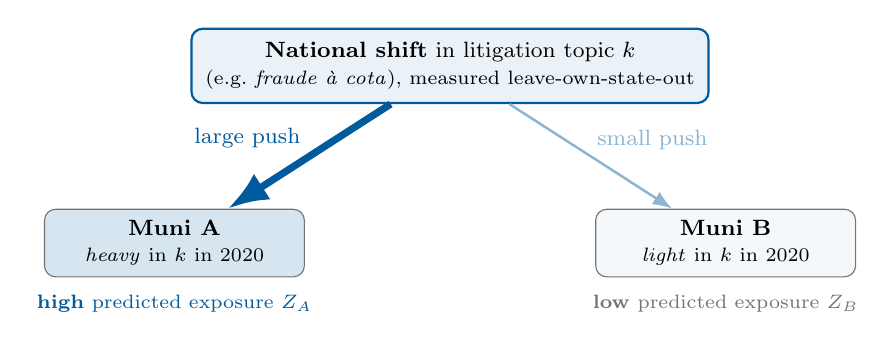
\begin{tikzpicture}[
  font=\footnotesize,
  wave/.style={draw=myblue, thick, rounded corners, fill=myblue!8, align=center, inner sep=5pt},
  muni/.style={draw=black!55, rounded corners, align=center, inner sep=4pt, minimum width=3.3cm},
  hi/.style={-{Latex}, myblue, line width=2.6pt},
  lo/.style={-{Latex}, myblue!45, line width=0.9pt},
]
  \node[wave] (nat) at (0,2.25) {\textbf{National shift} in litigation topic $k$\\ \scriptsize (e.g.\ \emph{fraude \`a cota}), measured leave-own-state-out};
  \node[muni, fill=myblue!16] (a) at (-3.5,0) {\textbf{Muni A}\\ \scriptsize \emph{heavy} in $k$ in 2020};
  \node[muni, fill=myblue!4]  (b) at (3.5,0)  {\textbf{Muni B}\\ \scriptsize \emph{light} in $k$ in 2020};
  \draw[hi] (nat) -- (a) node[midway,above left=-2pt]{large push};
  \draw[lo] (nat) -- (b) node[midway,above right=-2pt]{small push};
  \node[below=3pt of a, myblue]   {\scriptsize \textbf{high} predicted exposure $Z_A$};
  \node[below=3pt of b, black!55] {\scriptsize \textbf{low} predicted exposure $Z_B$};
\end{tikzpicture}
\end{center}
\vspace{2pt}
\centerline{\footnotesize The comparison is between municipalities pushed harder by \emph{identical} national trends.}
\smallskip
\footnotesize Two ingredients construct it: each municipality's 2020 caseload mix across litigation subjects, and the national shift in each subject measured leave-own-state-out. Both rest on a prior decision about which filings count as adversarial.
\end{frame}


\subsection{Sources}


\begin{frame}{Data Sources}
\hypertarget{src:datasources}{}

\vspace{2pt}
\centering
\scriptsize
\renewcommand{\arraystretch}{1.18}
\setlength{\tabcolsep}{6pt}
\begin{tabular}{L{5.6cm}L{2.4cm}C{1.9cm}L{2.4cm}}
  \toprule
  \textbf{Dataset} & \textbf{Source} & \textbf{Years} & \textbf{Use} \\
  \midrule

  % ---- LAWSUITS ----
  \rowcolor{bandlaw} \multicolumn{4}{l}{\textbf{Lawsuits}} \\
  \quad Electoral lawsuit filings & TSE (SIG export) & 2020, 2024 & Instrument \\
  \midrule

  % ---- CANDIDATES ----
  \rowcolor{bandcnd} \multicolumn{4}{l}{\textbf{Candidates}} \\
  \quad Candidate registry & TSE & 2012--2024 & Outcome \\
  \quad Election results & TSE & 2016--2024 & Outcome \\
  \quad Campaign finance (SPCE) & TSE & 2020, 2024 & Mechanism \\
  \midrule

  % ---- ELECTORATE ----
  \rowcolor{bandvot} \multicolumn{4}{l}{\textbf{Electorate}} \\
  \quad Turnout \& ballot composition & TSE & 2016--2024 & Outcome \\
  \quad Turnout by voter profile (\emph{perfil}) & TSE & 2020, 2024 & Outcome \\
  \midrule

  % ---- MUNICIPALITY CHARACTERISTICS ----
  \rowcolor{bandctl} \multicolumn{4}{l}{\textbf{Municipality characteristics}} \\
  \quad Census 2010 & IBGE & 2010 & Control \\

  \bottomrule
\end{tabular}

\medskip

{\raggedright\scriptsize
\textbf{Use:} Instrument = shift-share IV \,$\cdot$\, Outcome = causal estimand \,$\cdot$\, Mechanism = channel test \,$\cdot$\, Control = covariate.\\[3pt]
Two additions are pending. News-outlet coverage (Atlas da Not\'{i}cia, Volt Data Lab) and poll coverage (Poder360) would support the media-salience mechanism and heterogeneity by information environment. A pre-2018 lawsuit panel would support the $2016\to2020$ placebo; the LAI request for 2016 and 2012 is outstanding.\par}
\end{frame}


\subsection{What We Keep}


\begin{frame}{The Adversarial Filter: What Counts as Treatment}
\hypertarget{src:adversarialfilter}{}
\footnotesize
Most electoral filings are mandatory paperwork: one candidacy registration (RRC/DRAP) and one finance account (\emph{presta\c{c}\~ao de contas}) per candidate. These move one-for-one with the candidate pool and carry no adversarial signal. Treatment keeps only genuine contests between political actors.
\smallskip

\begin{center}
\renewcommand{\arraystretch}{1.15}
\resizebox{0.94\linewidth}{!}{%
\begin{tabular}{L{6.0cm}L{6.0cm}}
  \toprule
  \cellcolor{bandvot}\textbf{Kept: adversarial contests} & \cellcolor{bandlaw}\textbf{Dropped: administrative / procedural} \\
  \midrule
  Propaganda, disinformation, right of reply & Candidacy registration (RRC / DRAP) \\
  Abuse of economic / political power (AIJE, AIME) & Campaign-finance accounts (\emph{presta\c{c}\~ao de contas}) \\
  Campaign-finance \& poll-conduct disputes & Vote tallying \& poll-worker admin \\
  Registration \& eligibility \emph{challenges} (\emph{impugna\c{c}\~ao}, inelegibilidade) & Procedural acts \& enforcement (citation, \emph{cumprimento}) \\
  Originating electoral crimes (vote-buying, \emph{a\c{c}\~ao penal}) & Voter-roll, party-internal, fiscal tail \\
  \bottomrule
\end{tabular}}
\end{center}
\smallskip

\begin{itemize}\itemsep3pt
  \item A filing is routed by subject and gated by class: it is kept on what it is \emph{about}, while its criminal status follows the procedural vehicle. A registration \emph{challenge} therefore survives even inside the mandatory registration class.
  \item What remains is \KeptAdversarialLawsuits{} adversarial filings, \KeptAdversarialPct\% of the \TotalAllLawsuits{} million total. Treatment is $\Delta\log(1+\ell_m)$, the 2020$\to$2024 change in this count per municipality.
\end{itemize}
\end{frame}


\subsection{What We Measure}

\begin{frame}{Outcomes: Three Layers of the Contest}
\hypertarget{src:outcomes}{}
\small
The unit of analysis is the local election. We estimate whether adversarial litigation intensity changes the contest itself; who wins a given seat is not the object. Outcomes fall into three layers, each measured as a 2020--2024 change. Leveling and Barrier predict opposite signs in the first two layers, and the same sign in the third.
\vspace{10pt}
\begin{center}
\renewcommand{\arraystretch}{1.7}
\resizebox{\linewidth}{!}{%
\begin{tabular}{@{}l l c c@{}}
\toprule
 & Outcomes & \textcolor{mygreen}{Leveling predicts} & \textcolor{myred}{Barrier predicts} \\
\midrule
1\ \ Candidate supply & Entrants, women and non-white candidates, party count, field size & broader pool & fewer, safer names \\
2\ \ Voter response & Turnout, blank and null votes & engagement sustained & withdrawal \\
3\ \ Contest outcome & Top-two margin, effective number of candidates, incumbency advantage & ambiguous & consolidation \\
\bottomrule
\end{tabular}}
\end{center}
\vspace{10pt}
{\centering\footnotesize Only layer 2 discriminates. A narrower contest is consistent with either face, so the face is assigned on the ballot.\par}
\end{frame}



% ============================================================
% 4. EMPIRICAL STRATEGY
% Strategy states assumptions; Results shows estimates. The first stage is
% an estimate, so it lives in Sec. 5 with the other estimates.
% ============================================================
\section{Empirical Strategy}

\subsection{What We Estimate}
\input{frames/src_spec.tex}

\subsection{The Instrument}

\begin{frame}{Constructing the Instrument: Shares $\times$ Shifts}
\hypertarget{src:instrument}{}
\footnotesize
The instrument combines a pre-determined 2020 exposure share with a leave-own-state-out national shift, at the subject level (\NSubjectsKept{} kept TSE subjects; no family aggregation is imposed on $\bZ$).
\smallskip

\textbf{Shares:} each municipality's 2020 adversarial-subject mix, fixed two cycles before 2024 outcomes.
\[
s_{m,k,2020} \;=\; \frac{\text{adversarial lawsuits of subject } k \text{ in } m,\ 2020}{\text{all adversarial lawsuits in } m,\ 2020},
\qquad \sum_k s_{m,k,2020}=1.
\]
\textbf{Shifts:} each subject's log caseload growth, summed over all other states.
\[
g_{\text{UF}(m),\,k} \;=\; \log\!\bigl(1 + L_{-\text{UF},\,k,\,2024}\bigr) - \log\!\bigl(1 + L_{-\text{UF},\,k,\,2020}\bigr),
\qquad L_{-\text{UF},\,k,\,t} = L^{\text{nat}}_{k,t} - L^{\text{own-UF}}_{k,t}.
\]
\textbf{Instrument:} the portfolio-weighted predicted exposure, one number per municipality.
\[
\bZ \;=\; \sum_{k} \; \underbrace{s_{m,k,2020}}_{\text{share (pre-determined)}} \;\cdot\; \underbrace{g_{\text{UF}(m),\,k}}_{\text{shift (other states)}}
\]
\smallskip
\begin{itemize}\itemsep2pt
  \item Leaving out the own state removes local litigation shocks from the shift. A municipality's shift excludes its whole state, so every municipality in a state shares the same per-subject shift and state fixed effects absorb it. Identification therefore comes from within-state variation in the 2020 shares, and the adjudication locus (the zone) sits inside the state.
  \item The variation is off subjects that diffuse across states, such as jurisprudence, MPE priorities and party legal strategy, rather than off local politics. The same $\bZ$ is carried into the executive and legislative designs.
\end{itemize}
\end{frame}



\begin{frame}{The Instrument Across Brazil}
\hypertarget{src:instrumentmap}{}
\footnotesize
\begin{columns}[T]
\begin{column}{0.58\textwidth}
  \centering
  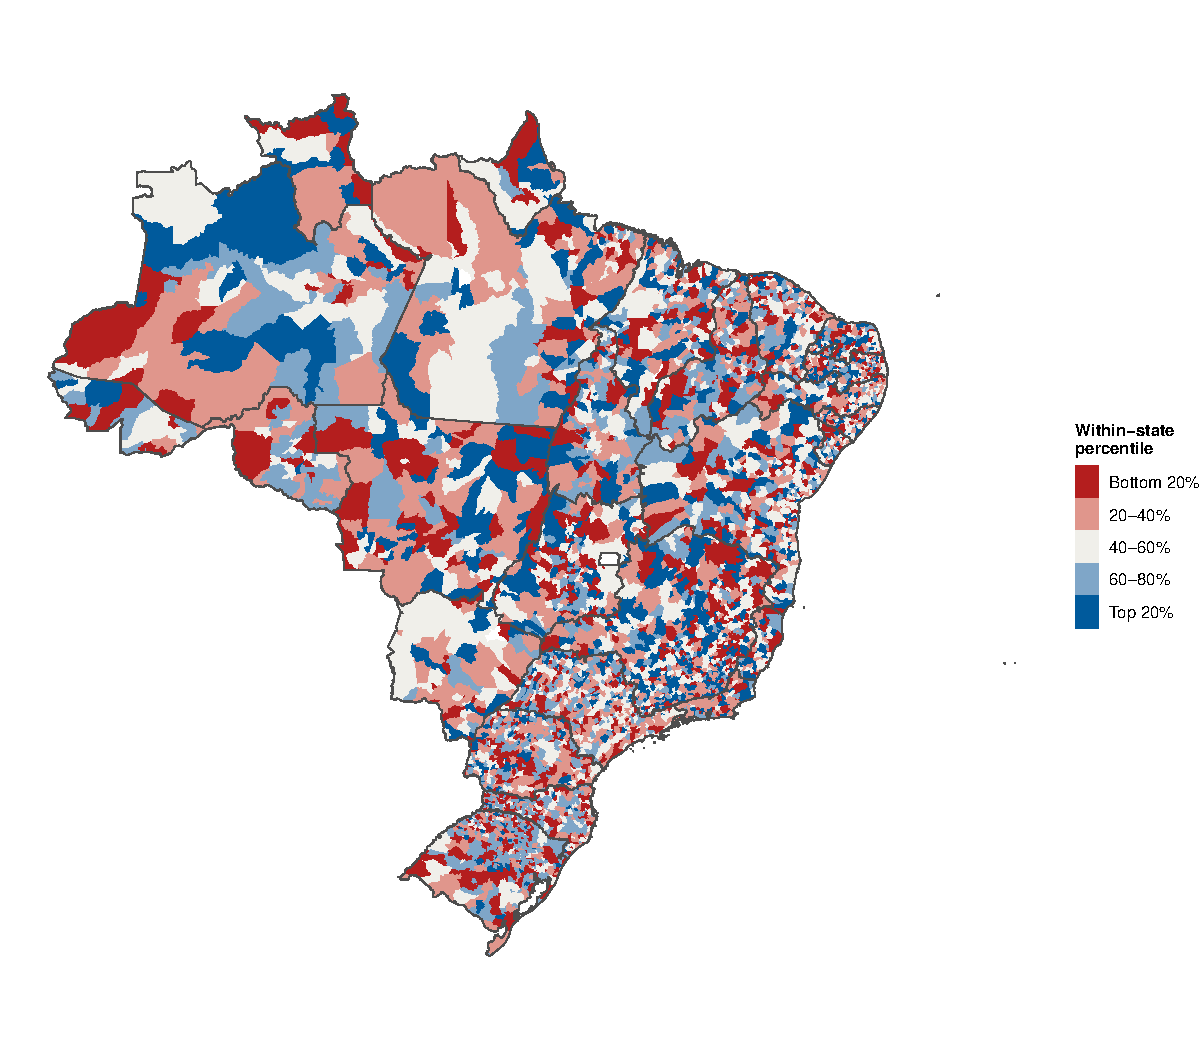
\includegraphics[width=\linewidth,height=0.60\textheight,keepaspectratio]{../figures/instrument_map.pdf}\\[4pt]
  {\scriptsize\ns{Predicted exposure by municipality. \textcolor{myblue}{Blue} = above-average, \textcolor{myred}{red} = below-average.}}
\end{column}
\begin{column}{0.40\textwidth}
  \centering
  \vspace{0.06\textheight}
  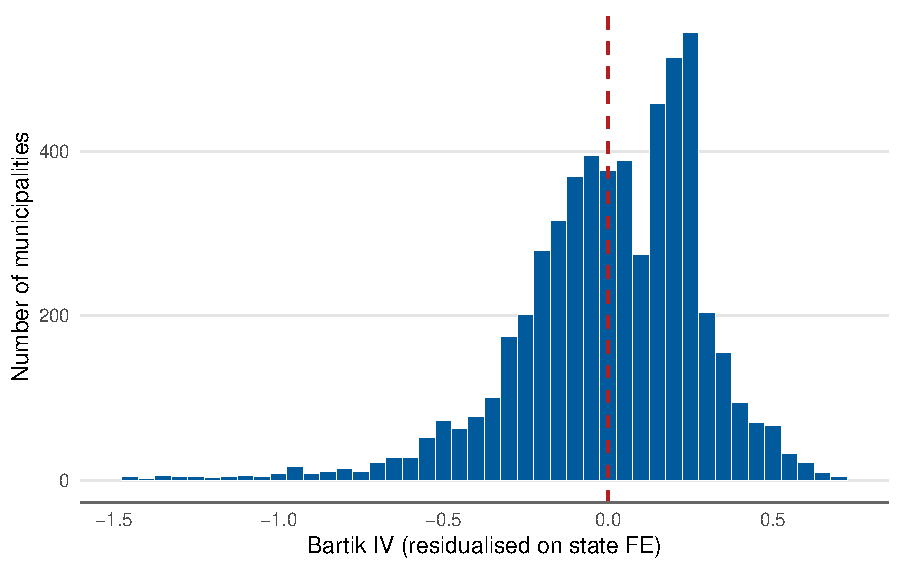
\includegraphics[width=\linewidth,height=0.42\textheight,keepaspectratio]{../figures/instrument_histogram.pdf}\\[4pt]
  {\scriptsize\ns{Instrument after removing state fixed effects. Identifying variation is \textbf{within-state} (SD $=\BartikZSDResid$).}}\\[10pt]
  \raggedright\scriptsize A heavier campaign-conduct / information-environment mix in 2020 means higher predicted litigation exposure by 2024.
\end{column}
\end{columns}
\end{frame}



% [2026-07-02 consolidation] Old "Clustering and the Few-Clusters Caveat" frame removed; its content is reconciled and merged into the "Inference: Few Clusters and the Exposure-Robust Bound" frame placed after the shares-defense frame. The fix corrects two stale claims: (i) the mayoral blank rate straddles zero (p=ARBlankP=0.108), it does NOT exclude zero; (ii) the exposure-robust bound inflates the margin SE by only ERMarginRatio=1.06x, so the consolidation DOES clear it.


% [2026-07-02 consolidation] "The First Stage, Visually" frame removed; the binscatter (firststage_linear.pdf) is now the right-hand column of the first-stage frame (frames/src_firststage.tex).


\subsection{Identification \& Inference}

\begin{frame}{Identification and Inference}
\hypertarget{src:identbrief}{}
\small
The instrument is share-identified. With only $K_{\text{eff}}=\KeffRotemberg$ effective shocks, credibility rests on the exogeneity of the 2020 caseload shares rather than on averaging many independent shifters \citep{goldsmith2020,borusyak2022}. Three checks carry it, each with a full appendix.
\medskip
\begin{itemize}\itemsep4pt
  \item A handful of national \emph{propaganda}-regulation shocks carry most of the Rotemberg weight: \RotPropTopFive{} of the five highest-weight subjects are propaganda subjects, and their own $F_k$ ranges from \RotFMin{} to \RotFMax{}. \hfill\hyperlink{app:rotemberg}{\beamergotobutton{Rotemberg weights}}
  \item The shares carry the adversarial signal specifically. Conditioning on non-adversarial filing intensity leaves the estimate unmoved, and a placebo Bartik built from the excluded mandatory filings is null. \hfill\hyperlink{app:shares}{\beamergotobutton{Defending the shares}}
  \item Inference is robust to weak instruments and few clusters. State clustering leaves \NClusters{} clusters, so headline $p$-values come from an Anderson--Rubin wild-cluster bootstrap \ns{\citep{andersonrubin1949,roodman2019}}, and a BHJ/AKM exposure-robust bound \ns{\citep{borusyak2022,adao2019}} barely moves the margin SE. \hfill\hyperlink{app:inference}{\beamergotobutton{Inference}}
\end{itemize}
\smallskip
\takeaway{Every result below uses one estimator: 2SLS of the outcome on instrumented $\Delta\log(1+\text{adversarial lawsuits})$, each outcome the 2024 value on its 2016 baseline (ANCOVA), with state fixed effects and state-clustered standard errors. In every coefficient plot the thick bar is the 90\% CI, the thin bar the weak-IV $tF$ 95\% CI, and \textcolor{myred}{\textbf{red}} marks conventional $p<.05$. Plotted coefficients are per unit of $\Delta\log(1+\text{lawsuits})$; magnitudes in the text are per one-SD rise in judicialization ($\approx\TreatSDMult\times$ litigation).}
\end{frame}

% TO BUILD -- src_compliers.tex: names the complier population in the MAIN
% section. The first stage lives entirely on zero-vs-any 2020 litigation
% (the intensive margin is a real null, PPML/NegBin p=.37/.08), so the
% estimate is a LATE for ONSET compliers. That is what the number means,
% not a robustness check; app_extensive stays as its supporting evidence.


% ============================================================
% 5. RESULTS
% From here the document turns to the second stage: what the instrumented
% change in adversarial litigation does to voters and candidates.
%
% Subsections are SUBSTANTIVE, not tiered -- grouping by confidence tier is
% harder to misread but destroys the candidates -> voters -> outcome spine,
% and this deck exists to be an argument. The rule that replaces it:
% NO FRAME SHIPS WITHOUT ITS CONFIDENCE TIER STATED ON THE FRAME.
%
% Frame order follows the outcome LAYERS defined in src_outcomes: layer 3
% (how open the contest stays) is the result; layers 1-2 (who runs, how
% voters respond) are the engines.
% ============================================================
\section{Results}

% ============================================================
\subsection{The First Stage}
% Its own subsection, not an opener to "The Result": the coefficient is
% positive, but it is identified on the extensive margin. Municipalities with
% no adversarial litigation in 2020 (Z = 0) gain filings; litigating ones
% lose them, with no gradient across nonzero exposure. The compliers are
% municipalities where litigation starts, not places where it amplifies.
% Miss that and every complier statement is misread.


\begin{frame}{Constructed Exposure Moves Realized Litigation}
\hypertarget{src:firststage}{}
\footnotesize
Regressing the 2020$\to$2024 change in adversarial filings on $\bZ$, with controls and state fixed effects, gives a precise positive coefficient and a cluster-robust effective $F=\HeadlineF$, far above the weak-instrument threshold. Inference uses the $tF$ correction \citep{lee2022}.
\smallskip
\begin{columns}[T]
\begin{column}{0.52\textwidth}
\centering
\resizebox{\linewidth}{!}{% Auto-generated by code/03_estimation/02_iv_main.R
% Do not edit manually -- rerun the generating script to update

\begin{tabular}{l*{4}{c}}
\toprule\toprule
Design: & \textbf{Baseline} & \textbf{Ext.\ controls} & \textbf{Open seats} & \textbf{Contested} \\
\midrule
\rowcolor{mylight}
\textbf{Predicted judicialization} & 0.418$^{***}$ & 0.405$^{***}$ & 0.393$^{***}$ & 0.425$^{***}$ \\
\rowcolor{mylight}
 & \textcolor{mygray}{(0.041)} & \textcolor{mygray}{(0.042)} & \textcolor{mygray}{(0.091)} & \textcolor{mygray}{(0.053)} \\
\midrule
First-stage $F$ & 102.3 & 93.3 & 18.6 & 65.1 \\
$N$ & 5,560 & 5,560 & 2,026 & 3,534 \\
\bottomrule\bottomrule
\end{tabular}
}\\[8pt]
\raggedright\scriptsize Coefficient $\FSCoef$ is the rise in $\Delta\log(1+\text{lawsuits})$ per unit of exposure. It is stable under the full control set (col.\ 2) and reproduces in each seat-type subsample (cols.\ 3--4).
\end{column}
\begin{column}{0.46\textwidth}
\centering
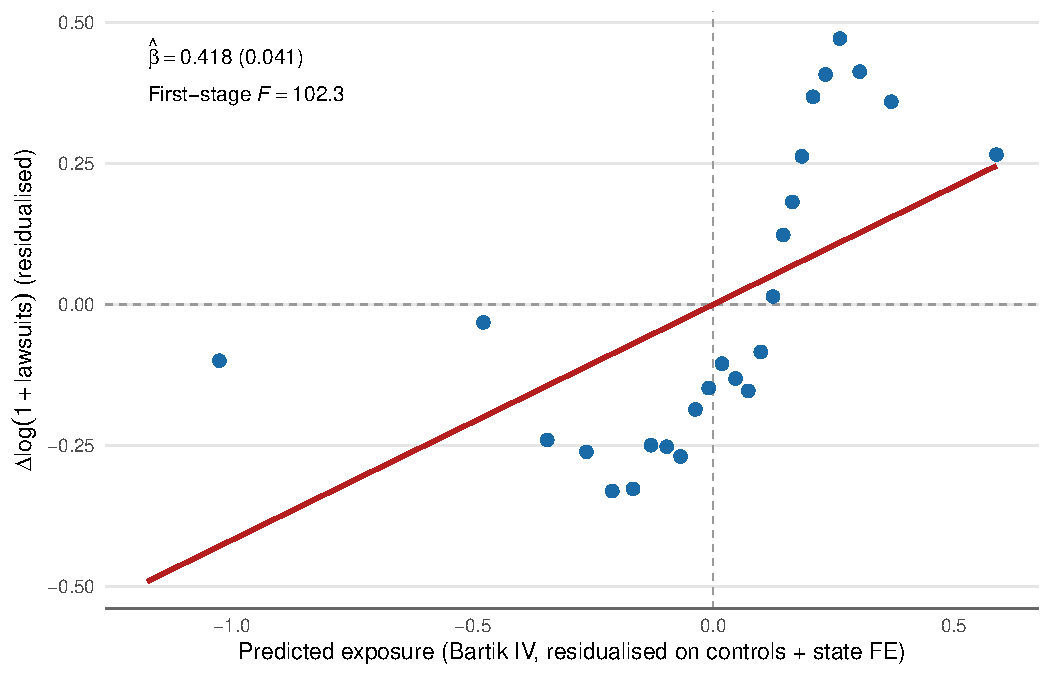
\includegraphics[width=\linewidth,height=0.52\textheight,keepaspectratio]{../figures/firststage_linear.pdf}\\[4pt]
\raggedright\scriptsize Realized growth against predicted exposure, both residualized on controls and state fixed effects (25 equal-count bins). The relationship is a single line through the origin, slope $\hat\beta=\FSCoef$.
\end{column}
\end{columns}
\smallskip
\centerline{\hyperlink{app:extensive}{\beamergotobutton{Zero-vs-any litigation?}}\quad\hyperlink{app:reclass}{\beamergotobutton{A coding artifact?}}}
\end{frame}



% ============================================================
\subsection{What the Contest Produces}

\begin{frame}{Candidates, Voters, and What the Contest Produces}
\hypertarget{src:story}{}
\small
An election is produced by two behaviors: candidates decide whether to run and how to campaign, and voters decide whether to turn out and how to mark the ballot. We isolate the contest's judicial dimension and ask how each side responds and what the two jointly produce.
\vspace{-4pt}
\begin{center}
\scalebox{0.94}{
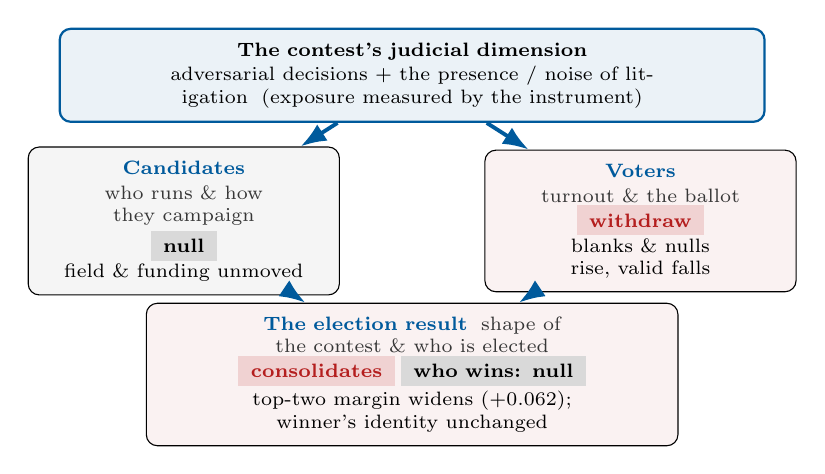
\begin{tikzpicture}[
  font=\scriptsize,
  exp/.style={draw=myblue, thick, rounded corners, fill=myblue!8, align=center, inner sep=5pt, text width=8.6cm},
  eng/.style={draw, rounded corners, align=center, inner sep=5pt, minimum height=1.75cm, text width=3.6cm},
  res/.style={draw, rounded corners, align=center, inner sep=5pt, minimum height=1.4cm, text width=6.4cm},
  flow/.style={-{Latex}, myblue, line width=1.4pt},
]
  \node[exp] (exp) at (0,2.25)
    {\textbf{The contest's judicial dimension}\\[1pt]adversarial decisions $+$ the presence / noise of litigation \;(exposure measured by the instrument)};
  \node[eng, fill=mygray!8] (cand) at (-2.9,0.4)
    {\textcolor{myblue}{\textbf{Candidates}}\\[1pt]\ns{who runs \& how they campaign}\\[1pt]
     \colorbox{mygray!30}{\textbf{\,null\,}}\\[1pt]
     {field \& funding unmoved}};
  \node[eng, fill=myred!6] (vot) at (2.9,0.4)
    {\textcolor{myblue}{\textbf{Voters}}\\[1pt]\ns{turnout \& the ballot}\\[1pt]
     \colorbox{myred!20}{\textcolor{myred}{\textbf{\,withdraw\,}}}\\[1pt]
     {blanks \& nulls rise, valid falls}};
  \node[res, fill=myred!6] (res) at (0,-1.55)
    {\textcolor{myblue}{\textbf{The election result}} \;\ns{shape of the contest \& who is elected}\\[1pt]
     \colorbox{myred!20}{\textcolor{myred}{\textbf{\,consolidates\,}}}\;\colorbox{mygray!30}{\textbf{\,who wins: null\,}}\\[1pt]
     {top-two margin widens ($\MarginCoef$); winner's identity unchanged}};
  \draw[flow] (exp) -- (cand);
  \draw[flow] (exp) -- (vot);
  \draw[flow] (cand) -- (res);
  \draw[flow] (vot) -- (res);
\end{tikzpicture}
}
\end{center}
\vspace{-4pt}
\footnotesize The candidate side is quiet while voters withdraw where an incumbent is defended. The consolidation is general across seat types and comes from the electorate re-allocating toward the leader rather than from candidates being removed. A narrower contest does not by itself name a face, so the barrier reading rests on the ballot, and the council race is null throughout.
\end{frame}

% ============================================================

\begin{frame}{The Mayoral Race Consolidates: the Top-Two Margin Widens}
\hypertarget{src:spine1}{}
\small
The winner's vote share rises, the runner-up's falls, and the top-two margin between them widens. All three point toward consolidation, and this is the headline result.
\smallskip
\begin{center}
\scriptsize
\resizebox{\linewidth}{!}{% Auto-generated by code/03_estimation/02_iv_main.R
% Do not edit manually -- rerun the generating script to update

\begin{tabular}{lccccc}
   \tabularnewline \midrule \midrule
   Dependent Variables:                                                     & delta\_runnerup\_vote\_share\_2024\_2020      & delta\_margin\_top1\_top2\_2024\_2020      & delta\_winner\_vote\_share\_2024\_2020      & delta\_winner\_majority\_2024\_2020     & delta\_log1p\_n\_candidates\_with\_votes\_2024\_2020\\         
   Model:                                                                   & (1)                                           & (2)                                        & (3)                                         & (4)                                     & (5)\\  
   \midrule
   \emph{Variables}\\
   $\Delta$ Log(lawsuits)                                                   & -0.031                                        & 0.062                                      & 0.031                                       & 0.140                                   & -0.066$^{\dagger}$\\    
                                                                            & (0.022)                                       & (0.043)                                    & (0.025)                                     & (0.090)                                 & (0.039)\\   
   \midrule
   \emph{Fixed-effects}\\
   SG\_UF                                                                   & Yes                                           & Yes                                        & Yes                                         & Yes                                     & Yes\\  
   \midrule
   \emph{Fit statistics}\\
   F-test (1st stage), delta\_log1p\_competition\_lawsuits\_2024\_2020      & 238.9                                         & 238.9                                      & 238.9                                       & 238.9                                   & 238.9\\  
   Observations                                                             & 5,560                                         & 5,560                                      & 5,560                                       & 5,560                                   & 5,560\\  
   \midrule \midrule
   \multicolumn{6}{l}{\emph{Clustered (cluster\_id) standard-errors in parentheses}}\\
   \multicolumn{6}{l}{\emph{Signif. Codes: **: 0.01, *: 0.05, \dagger: 0.1}}\\
\end{tabular}
}
\end{center}
\smallskip
\takeaway{A one-SD rise in judicialization widens the winner's margin by $+\MarginPerSD$~pp ($p=\MarginP$), lifts the winner's share by $+\WinSharePerSD$~pp, and cuts the runner-up's by $\RunnerUpPerSDSigned$~pp. Margin and runner-up both clear the weak-IV-robust AR bootstrap (margin $\ARMarginCI$, $p=\ARMarginP$), which is the inference the finding rests on.}
\smallskip
\scriptsize\ns{Whole-field concentration points the same way but is individually imprecise \hyperlink{app:concentration}{\beamergotobutton{whole-field}}; discretizations appendixed \hyperlink{app:compbinary}{\beamergotobutton{closeness}}.}\hfill\hyperlink{app:multiplicity}{\beamergotobutton{multiple testing \& index}}
\end{frame}



\begin{frame}{The Gender Incidence of the Consolidation}
\hypertarget{src:gender}{}
\small
A net effect can hide an offsetting transfer, so we open the consolidation itself. It moves vote from the runner-up's slot to the winner's; splitting both slots by the office-seeker's gender asks who pays and who collects. The split is unconditional: the components sum back exactly to the totals on the previous frames, with the same $N$ and nothing conditioned on who placed where \hyperlink{app:gender}{\beamergotobutton{construct \& full tables}}.
\smallskip
\begin{center}
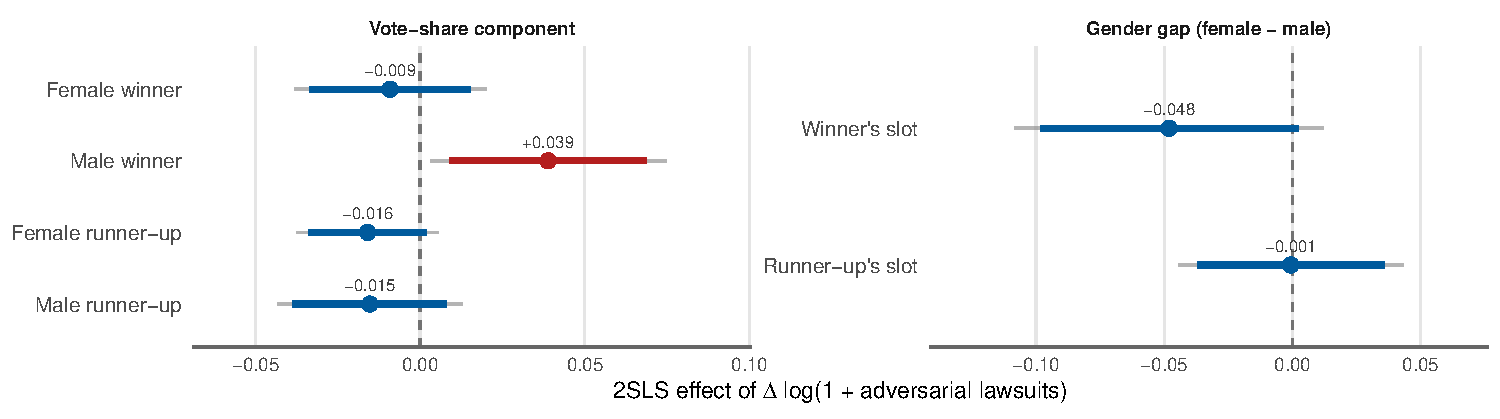
\includegraphics[width=\linewidth,height=0.32\textheight,keepaspectratio]{../figures/gender_consolidation_coefplot.pdf}
\end{center}
\smallskip
\takeaway{The cost is gender-neutral, while the gain may not be. The runner-up's loss splits evenly (female $\FemRUSharePerSDSigned$~pp, male $\MaleRUSharePerSDSigned$~pp) and that slot's gap is a precisely estimated zero ($\RUGapCoef$, $p=\RUGapP$) rather than an inconclusive one. The gain lands on male front-runners ($\MaleWinSharePerSDSigned$~pp, $p=\MaleWinShareP$) while the female winner's share is flat ($p=\FemWinShareP$), but that slot's differential test is $\WinGapPerSDSigned$~pp, $p=\WinGapP$: \negt{suggestive, not established}. Net, women's share of the top two drifts down $\FemTopTwoPerSDSigned$~pp ($p=\FemTopTwoP$).}
\smallskip
\scriptsize\ns{This is the incidence the demographic profile of the top two implies: if winner and runner-up are near-twins \hyperlink{src:favored}{\beamergotobutton{who it favors}}, widening the margin between them should be gender-blind on the losing side, and it is. Exploratory, outside the declared family, raw $p$ \hyperlink{app:multiplicity}{\beamergotobutton{multiplicity}}.}
\end{frame}



% ============================================================
\subsection{Candidates and Voters}


\begin{frame}{The Consolidation Favors the Incumbent}
\hypertarget{src:favored}{}
\small
Consolidation reinforces whoever is already ahead, and the 2024 mayoral field identifies who that is descriptively, before any regression. Profiling candidates by within-race vote rank shows that the winner and the runner-up part on political standing rather than demographics. The front-runner is a sitting incumbent roughly five times as often; on gender, race, education and age the top two are near-twins.
\smallskip
\begin{center}
\scriptsize
\resizebox{!}{0.23\textheight}{% Auto-generated by code/04_analysis/10_candidate_rank_profile.py (2024 mayoral)
% Do not edit manually -- rerun the generating script to update

\begin{tabular}{lccc}
\toprule\toprule
 & \textbf{Winner} & \textbf{Runner-up} & \textbf{Rest of} \\
 & \scriptsize{(1st)} & \scriptsize{(2nd)} & \scriptsize{field} \\
\midrule
\multicolumn{4}{l}{\textit{Political standing}} \\
\rowcolor{mylight}
\quad Incumbent (won this seat last cycle) & 42.2 & 7.7 & 1.1 \\
\quad Prior election winner & 65.1 & 48.9 & 28.5 \\
\quad First-time candidate & 25.0 & 32.7 & 42.6 \\
\midrule
\multicolumn{4}{l}{\textit{Demographics}} \\
\quad Female & 13.2 & 17.1 & 16.4 \\
\quad Non-white & 33.9 & 35.7 & 39.0 \\
\quad Higher education & 64.2 & 62.6 & 65.7 \\
\quad Age (years) & 50.0 & 51.0 & 51.5 \\
\midrule
$N$ candidates & 5,560 & 5,331 & 4,141 \\
\bottomrule\bottomrule
\end{tabular}
}
\end{center}
\smallskip
\takeaway{Because the top two are demographically interchangeable, widening the margin between them entrenches incumbency, which is a politically rather than demographically defined trait. This is mechanically why the vote-weighted gender and race composition of winners cannot move: what the consolidation protects is incumbency. \ns{Descriptive shares by vote rank; no causal content.}}
\end{frame}



\begin{frame}{Litigation Does Not Reshape Who Wins the Mayoral Race}
\hypertarget{src:representation}{}
\small
If consolidation moves the margin but leaves identities intact, the vote-weighted composition of winners should be flat, and it is. The vote-weighted gender, race and incumbency mix, along with the winner's own identity, do not move significantly. Entrant typology \hyperlink{src:entrant}{\beamergotobutton{here}}.
\smallskip
\begin{center}
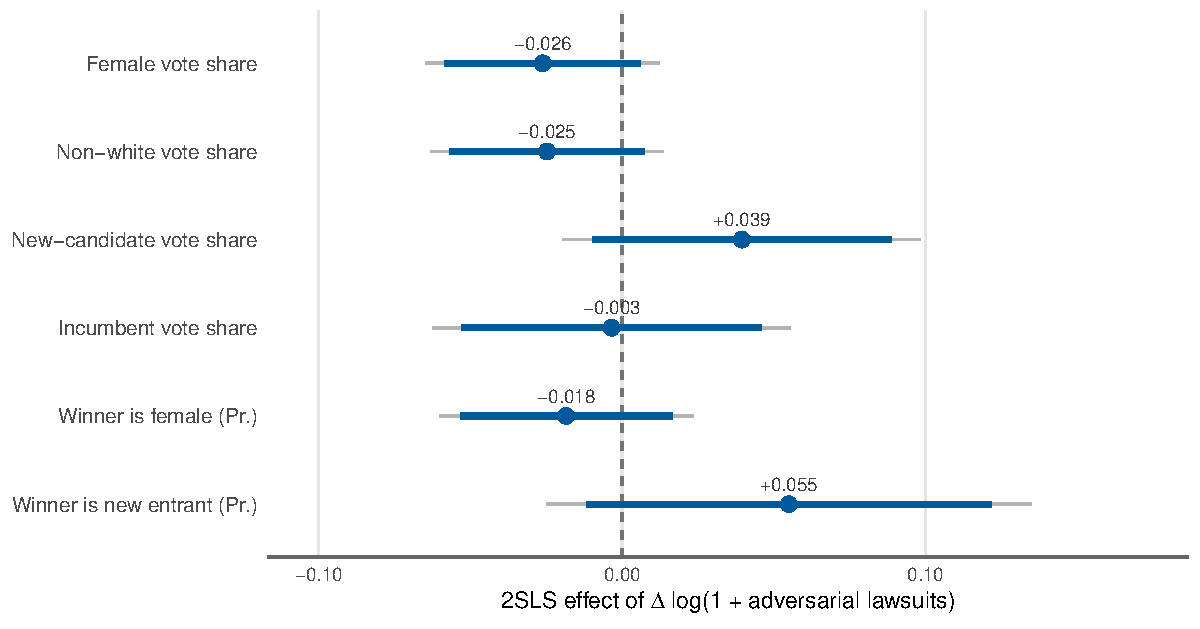
\includegraphics[width=\linewidth,height=0.46\textheight,keepaspectratio]{../figures/representation_coefplot.pdf}
\end{center}
\smallskip
\takeaway{Every interval straddles zero: a one-SD shock moves the female vote share by $\FemaleVSPerSDSigned$~pp and the probability the winner is female by $\FemaleWinPerSDSigned$~pp, neither distinguishable from zero. Litigation neither advances nor suppresses descriptive representation on net.}\hfill\hyperlink{app:representation}{\beamergotobutton{Full table}}
\end{frame}

% ============================================================

\begin{frame}{Candidate Supply Does Not Move, in Either Office}
\hypertarget{src:candidates}{}
\small
Litigation could thin the field as a \negt{barrier}, since suits are costly to mount and defend, or open it as a weapon, since a credible threat of challenge can deter a front-runner from standing. The sign is therefore ambiguous \emph{a priori}. Entry is also an anticipation margin: candidacies register at the August deadline \ns{(Lei 9.504, art.~11)}, before most suits resolve. Neither force shows up in the mayoral field or in the size of the council field.
\smallskip
\begin{center}
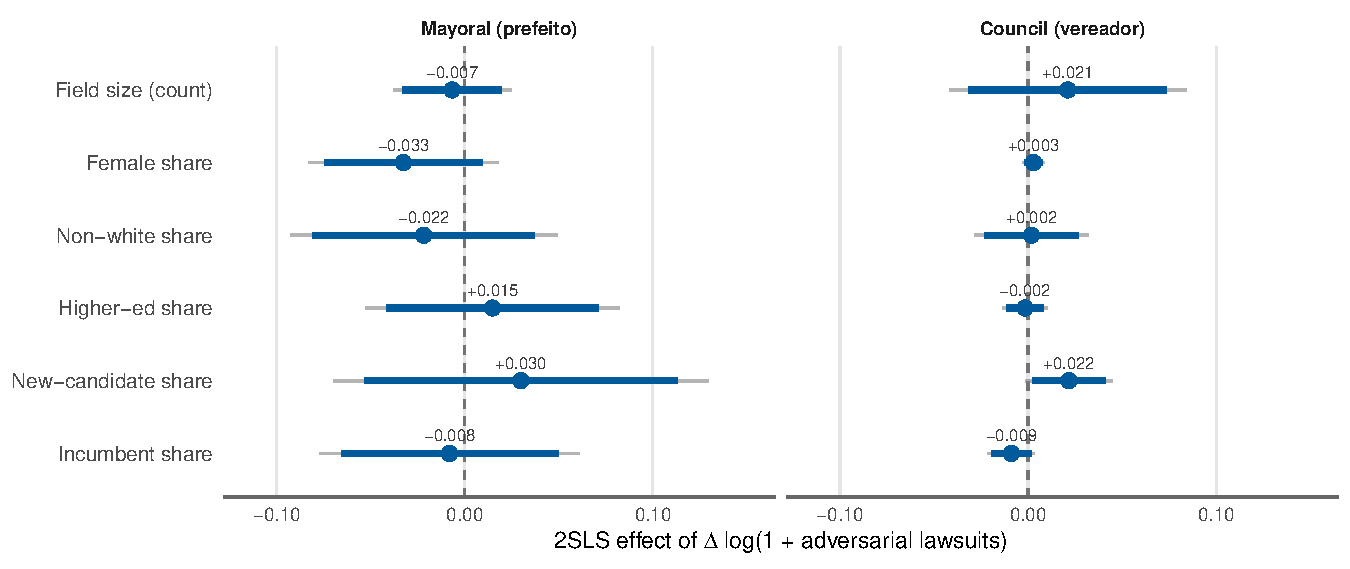
\includegraphics[width=\linewidth,height=0.44\textheight,keepaspectratio]{../figures/candidate_supply_coefplot.pdf}
\end{center}
\smallskip
\takeaway{No plotted supply margin moves in either office: mayoral field size ($\CandExecCoef$, $p=\CandExecP$), its female ($\FemaleCandCoef$, $p=\FemaleCandP$), non-white, higher-ed, new-entrant and incumbent shares, and the council pool ($\LegCandCoef$, $p=\LegCandP$) all straddle zero. Mean age is flat in the mayoral field (\MayorAgeYr~yr); the council pool is younger (\CouncilAgeYr~yr, $p=\CouncilAgeP$), one of \CouncilNSig{} of \CouncilNOutcomes{} council outcomes that clear 5\%; no council multiplicity correction is computed. What reshapes the race is therefore voter behavior, not the composition of the field.}\hfill\hyperlink{app:compbinary}{\beamergotobutton{count table}}
\end{frame}



\begin{frame}{Litigation Pushes Voters Off the Mayoral Ballot}
\hypertarget{src:voterballot}{}
\small
Turnout is compulsory in Brazil for literate voters aged 18--69 \ns{(CF/88 art.~14 \S1)} and so is institutionally floored, but a voter can still decline to choose, casting a blank or null ballot that elects no one. With turnout floored, demobilization would appear as a rise in these non-valid votes and a fall in valid ones. The mayoral estimates below carry that sign pattern, and only the blank rise approaches significance.
\smallskip
\begin{center}
\scriptsize
\resizebox{!}{0.22\textheight}{% Auto-generated by code/03_estimation/02_iv_main.R
% Do not edit manually -- rerun the generating script to update

\begin{tabular}{lccc}
\toprule\toprule
 & \textbf{Blank vote} & \textbf{Null vote} & \textbf{Valid vote} \\
\midrule
\rowcolor{mylight}
\quad \textbf{Judicialization} & $0.003$$^{*}$ & $0.003$ & $-0.007$ \\
\rowcolor{mylight}
 & \textcolor{mygray}{(0.002)} & \textcolor{mygray}{(0.002)} & \textcolor{mygray}{(0.006)} \\
\quad {\footnotesize 2024 Mean} & {\footnotesize 0.016} & {\footnotesize 0.027} & {\footnotesize 0.792} \\
\quad {\footnotesize 2016 Mean} & {\footnotesize 0.016} & {\footnotesize 0.051} & {\footnotesize 0.789} \\[2pt]
\midrule
Municipalities ($N$) & \multicolumn{3}{c}{5,560} \\
\bottomrule\bottomrule
\end{tabular}
}
\end{center}
\smallskip
\takeaway{A one-SD shock raises the mayoral blank rate by $+\BlankPerSD$~pp and the null rate by $+\NullPerSD$~pp, cutting valid votes by $\ValidPerSDSigned$~pp. The blank rise clears the exposure-robust SE ($p=\ERBlankPbhj$), is conventional only at 10\% ($p=\BlankP$), and fails the weak-IV AR bootstrap ($p=\ARBlankP$). Null ($p=\NullP$) and valid ($p=\ValidP$) share the sign pattern without significance. In contested seats the blank rise clears 5\% ($p=\ContBlankP$). The mayoral valid rate fails the pre-trend placebo ($p=\PtRFValidP$). The council ballot is flat.}\hfill\hyperlink{app:turnoutplacebo}{\beamergotobutton{turnout placebo}}\,\hyperlink{app:councilplacebo}{\beamergotobutton{council placebo}}
\end{frame}



% ============================================================
\subsection{Heterogeneity by Seat Type}
% ============================================================

\begin{frame}{Which Face, by Seat Type}
\hypertarget{src:seathet}{}
\small
Mayoral races split by whether the seat is open, meaning the incumbent is term-limited so no front-runner defends it ($N=2{,}026$), or contested, where the sitting mayor may still seek re-election ($N=3{,}534$). This split is what assigns the face. The margin widens in both, so only the ballot separates them.
\smallskip
\begin{center}
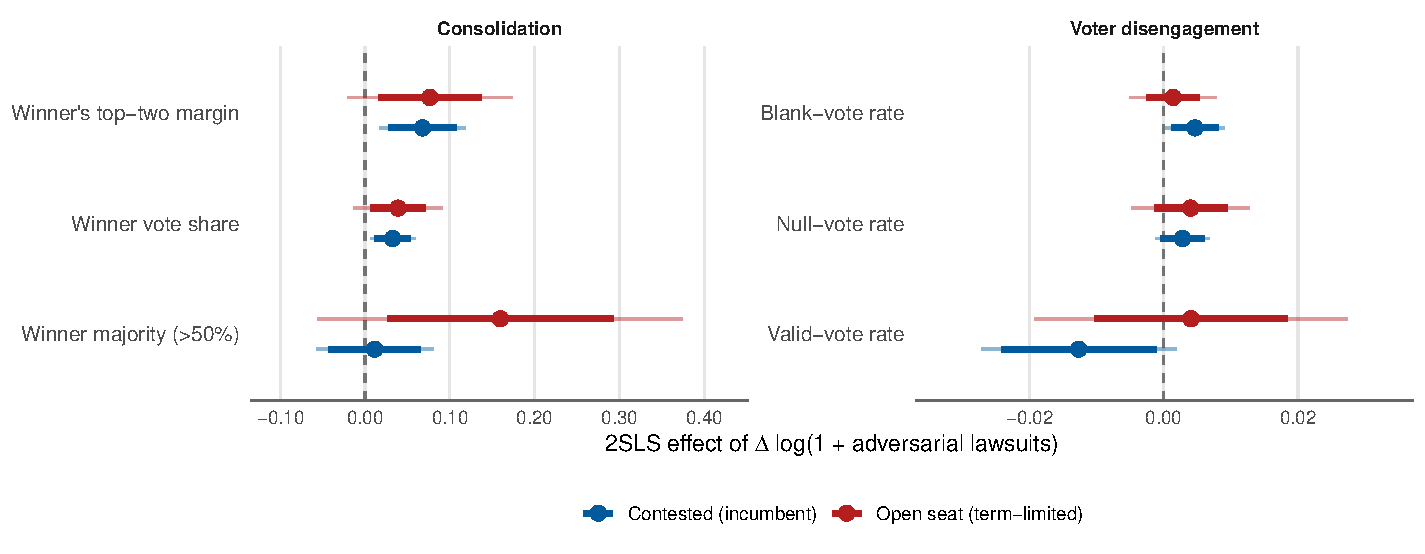
\includegraphics[width=\linewidth,height=0.44\textheight,keepaspectratio]{../figures/heterogeneity_seat_coefplot.pdf}
\end{center}
\smallskip
\takeaway{The winner's top-two margin widens in both seat types ($+0.076$, $p=.05$ open; $+0.068$, $p=.01$ contested), so the consolidation is general. The mechanism splits by seat. In open seats it is \pos{decisiveness}: the winner crosses 50\% ($+0.160$, $p=.06$) with no ballot demobilization. In contested seats it carries a \negt{barrier} signature: blank votes rise ($+0.005$, $p=.04$) and valid votes fall ($-0.013$, $p=.08$) as voters confront an entrenched incumbent, with no majority shift ($p=.74$). The same shock produces decisiveness where the seat is open and disengagement where it is defended.}\hfill\hyperlink{app:seathet}{\beamergotobutton{full table}}
\end{frame}



% ============================================================
% 6. ROBUSTNESS
% PRE-TRENDS ONLY in the main section, for now. The primary results are not
% final, and robustness architecture built on a moving headline gets redone.
%
% Promotion criterion, agreed 2026-08-12: a check earns a main frame if,
% left unaddressed, a referee stops believing the headline. Two are queued
% against it and decided when the primary results lock -- app_exposure
% (BHJ/AKM exposure-robust SEs, the one binding ANCOVA caveat) and
% app_multiplicity (the margin clears Holm and BH on the reduced-form
% p-values, Romano-Wolf only at 10%, and no correction on the 2SLS p-values).
% ============================================================
\section{Robustness}
% ============================================================

\begin{frame}{Robustness: Four Threats and Their Verdicts}
\hypertarget{src:robustness}{}
\footnotesize
With few concentrated shocks, credibility rests on the targeted checks below.
\renewcommand{\arraystretch}{1.0}
\begin{center}
\scriptsize
\begin{tabular}{@{}>{\raggedright\arraybackslash}p{2.6cm} p{9.2cm} c@{}}
\toprule\toprule
\textbf{Threat} & \textbf{Check} & \textbf{Verdict} \\
\midrule
The identifying variation is not what we claim\par\vspace{3pt}\hyperlink{app:extensive}{\beamergotobutton{extensive}} \hyperlink{app:reclass}{\beamergotobutton{reclass}} &
Reduced form survives dropping every zero-litigation municipality and a presence dummy; count-native Poisson \ns{\citep{santossilva2006}} and NegBin confirm the weak intensive margin is a real null. &
\tick \\
\midrule
The treatment definition drives the result\par\vspace{3pt}\hyperlink{app:tdef}{\beamergotobutton{treat.\ def.}} &
The reduced form does not depend on the definition ($p=\TdefRFp$), and the 2SLS sign is positive under all \TdefNdefs{}. It clears 5\% under log1p, IHS and binary, but not under levels ($p=\TdefLevelsP$, $F=\TdefLevelsF$) or the rate ($p=\TdefRateP$, $F=\TdefRateF$), the two definitions with weak first stages. &
\tick \\
\midrule
The inference overstates precision\par\vspace{3pt}\hyperlink{app:exposure}{\beamergotobutton{weak-IV}} \hyperlink{app:fd}{\beamergotobutton{FD}} &
Consolidation clears the weak-IV-robust AR bootstrap \ns{\citep{andersonrubin1949,roodman2019}} and the BHJ/AKM exposure-robust SE \ns{\citep{borusyak2022,adao2019}}, whose CI excludes zero ($\ERMarginCI$). Pure first differences return $\FDMarginCoef$ ($p=\FDMarginP$). &
\tick \\
\midrule
The result is multiple testing\par\vspace{3pt}\hyperlink{app:multiplicity}{\beamergotobutton{mult.}} \hyperlink{app:pretrend}{\beamergotobutton{pre-trend}} &
Over the \RWFamilyN{} reduced forms the margin clears Holm ($p=\RFHolmMarginP$) and BH ($p=\RFBHMarginP$), and Romano--Wolf only at 10\% ($p=\RWMarginP$) \ns{\citep{holm1979,benjamini1995,romano2005}}; over the \MultFamilyN{} 2SLS $p$-values none survives (margin Holm $p=\MultMarginHolm$). The closeness ($p=\IdxClosenessP$) and overall ($p=\IdxOverallP$) indices clear. The consolidation measures pass the pre-trend placebo; turnout and the valid-vote rate do not. &
\tick \\
\bottomrule\bottomrule
\end{tabular}
\end{center}
\footnotesize The margin fails correction on the 2SLS $p$-values, the weak-first-stage definitions and pure first differences. The blank-vote rise clears the exposure-robust SE ($p=\ERBlankPbhj$) but not the AR bootstrap ($p=\ARBlankP$).
\end{frame}


\begin{frame}{The Margin Is Pre-Trend Clean; Turnout and Valid Votes Are Not}
\hypertarget{src:pretrend}{}
\small
A free 2016 lag raises a fair question: does the instrument load on municipalities already moving in the consolidating direction? To test this we regress the 2016$\to$2020 pre-period change on the instrument, conditioning only on pre-determined (2010 Census) covariates and state FE. A clean, share-exogenous design wants every coefficient near zero, since the shock should not predict past movement.
\smallskip
\begin{center}
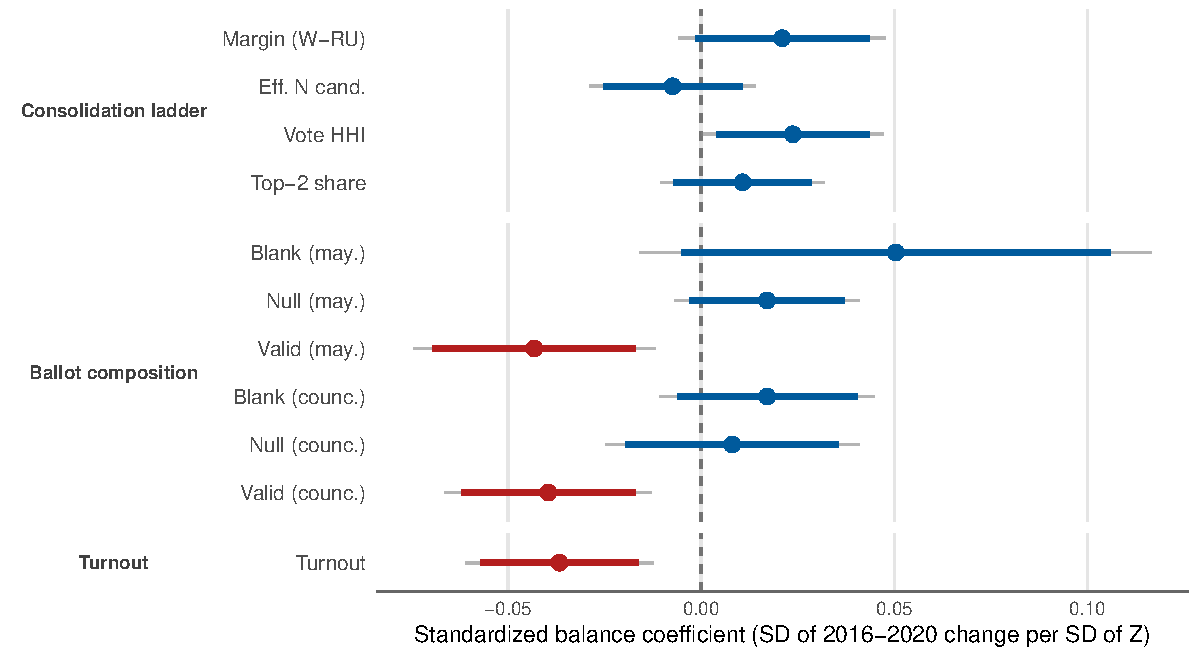
\includegraphics[width=\linewidth,height=0.44\textheight,keepaspectratio]{../figures/pretrend_coefplot.pdf}
\end{center}
\smallskip
\footnotesize Margin ($p=\PtRFMarginP$), effective-N ($p=\PtRFEffNP$) and top-two share ($p=\PtRFTopTwoP$) are clean; the Herfindahl is borderline ($p=\PtRFHHIP$, and tF rejects on the 2SLS placebo). Mayoral blank ($p=\PtRFBlankP$) and null ($p=\PtRFNullP$) are clean. \PtNFail{} of \PtNTests{} tests fail at 5\%: turnout ($p=\PtRFTurnoutP$), the mayoral valid rate ($p=\PtRFValidP$) and the council valid rate ($p=\PtRFValidVerP$). By seat, the margin pre-trends in open seats ($\OpenPtMarginCoef$, $p=\OpenPtMarginP$) and not in contested ones ($p=\ContPtMarginP$). Adding the 2020 level as a second lag moves the margin from $\MarginCoef$ to $\PtRobMarginCoef$ ($p=\PtRobMarginP$) \hyperlink{app:ptrobust}{\beamergotobutton{full pre-path}}. \emph{(Thick 90\%, thin 95\% CI; red $p<.05$.)}\hfill\hyperlink{app:pretrend}{\beamergotobutton{Placebo table}}
\end{frame}



% ============================================================
% 7. CONCLUSION
% [2026-08-12 spine] src_contribution.tex CUT. Under the Evans order in
% Sec. 1, "This Paper" states the contribution before the literature that
% positions it; restating it at the end was an artifact of the deck
% predating that reorder. What a conclusion adds that an introduction
% cannot is the conditions under which the paper fails -- so Limitations is
% the load-bearing frame, and its job is to name what would overturn the
% TENTATIVE face-assignment. The file was deleted 2026-09-16.
% ============================================================
\section{Conclusion}
% ============================================================

\begin{frame}{Findings by Confidence Tier}
\hypertarget{src:findings}{}
\footnotesize
On the clean 2016 baseline the evidence sorts into four tiers of confidence:
\smallskip
\begin{itemize}\itemsep1pt
  \item[\textcolor{myred}{\rule{1.2ex}{1.2ex}}] \textbf{Robust.} The mayoral race consolidates: the top-two margin widens ($\MarginCoef$, $p=\MarginP$), the winner's share rises ($\WinShareCoef$) and the runner-up's falls ($\RunnerUpCoef$). It clears the weak-IV-robust AR wild-cluster bootstrap (margin $p=\ARMarginP$, runner-up $p=\ARRunnerUpP$) and the BHJ/AKM exposure-robust SE (CI $\ERMarginCI$ excludes zero). Multiplicity depends on the basis: over the \RWFamilyN{} reduced forms the margin clears Holm ($p=\RFHolmMarginP$) and BH ($p=\RFBHMarginP$), and Romano--Wolf only at 10\% ($p=\RWMarginP$); over the \MultFamilyN{} 2SLS $p$-values nothing survives (margin Holm $p=\MultMarginHolm$, BH $p=\MultMarginBH$).
  \item[\textcolor{myred!55}{\rule{1.2ex}{1.2ex}}] \textbf{Tentative.} Voters withdraw from the mayoral ballot in contested seats: the blank rate rises ($\ContBlankCoef$, $p=\ContBlankP$) and the valid rate falls ($\ContValidCoef$, $p=\ContValidP$). Pooled, the blank rise ($\BlankCoef$) clears the exposure-robust SE ($p=\ERBlankPbhj$), is conventional only at 10\% ($p=\BlankP$) and fails the AR bootstrap ($p=\ARBlankP$); null ($p=\NullP$) and valid ($p=\ValidP$) are not significant.
  \item[\textcolor{mygray}{\rule{1.2ex}{1.2ex}}] \textbf{Nulls.} Descriptive representation and renewal, the entrant typology, elastic and education-stratified turnout, campaign finance, and the council ballot do not move. Two exceptions: \CouncilNSig{} of \CouncilNOutcomes{} council outcomes clear 5\% (elected female share $p=\CouncilElFemaleP$, pool age $p=\CouncilAgeP$; no council correction computed), and compulsory turnout rises ($\CompulsoryCoef$, $p=\CompulsoryP$, tF rejects). The consolidation's cost belongs here as well: the runner-up's loss splits evenly by gender ($\RUGapCoef$, $p=\RUGapP$) \hyperlink{src:gender}{\beamergotobutton{gender}}.
  \item[\textcolor{mygray!55}{\rule{1.2ex}{1.2ex}}] \textbf{Exploratory.} The winner's gain lands on male front-runners ($\MaleWinSharePerSDSigned$~pp, $p=\MaleWinShareP$) with the female winner's share flat, but the differential test does not clear ($p=\WinGapP$) and these outcomes sit outside the declared family. The data suggest the direction without establishing it.
\end{itemize}
\smallskip
\footnotesize The candidate side is quiet while some voters withdraw, so the consolidation is votes re-allocating toward the leader rather than candidates being removed. The consolidation is robust; the barrier reading sits one tier down because it rests on the ballot.\hfill\hyperlink{app:abstract}{\beamergotobutton{summary table}}\, \hyperlink{src:mechanism}{\beamergotobutton{mechanism}}
\end{frame}


\begin{frame}{Limitations}
\hypertarget{src:limitations}{}
\small
Four considerations bound the reach of the claim.
\medskip
\begin{enumerate}\itemsep4pt
  \item \textbf{Few effective shocks.} Identification rests on $K_{\text{eff}}=\KeffRotemberg$ effective shocks, with \RotPropagandaPct\% of the weight on propaganda subjects, and on \NClusters{} clusters. A many-shock law of large numbers \ns{\citep{borusyak2022}} does not apply, so the design is defended on the exogeneity of the 2020 shares rather than on shock count. That exogeneity is only partly supported: on unclustered tests, \GpsCovFail{} of \GpsNTopics{} tested topic shares correlate with the baseline controls, and \GpsMarginPtFail{} predict the 2016$\to$2020 margin change.
  \item \textbf{Extensive-margin identification.} The first stage moves the treatment on the extensive margin, so the per-unit-of-volume magnitude is not well identified even though the existence and sign of the effect are. The estimate is a local effect for onset compliers.
  \item \textbf{The face assignment is tentative.} The consolidation is robust, but which face produced it is assigned by the open-versus-contested split, and that split turns on ballot movement in contested seats that clears conventional and exposure-robust inference without clearing the AR bootstrap. If that ballot movement failed to replicate, the consolidation would survive and the barrier reading would not.
  \item \textbf{Aggregate, not case-level.} The treatment is municipal-level litigation intensity, not any single suit, so the design speaks to the aggregate climate of judicialization a race faces rather than to the outcome of a specific case.
\end{enumerate}
\end{frame}



% ============================================================
% APPENDIX
% Not a spine section. Collects every app_ frame the deck reaches by
% button, ordered by the main section that points into it.
% ============================================================
\section{Appendix}

\begin{frame}{Appendix --- Theoretical Framework: Signal vs Weapon}
\hypertarget{app:theory}{}
\footnotesize
The \textbf{Leveling} and \textbf{Barrier} faces of the main text rest on two hypotheses about \emph{why} litigation moves an election. A third channel --- \emph{direct judicial action}, where a ruling removes a candidate and mechanically reallocates the vote --- lies \textbf{outside the estimand}: the adversarial filter drops the candidacy-registration and campaign-finance machinery (RRC/DRAP, \emph{presta\c{c}\~ao de contas}), so it is not what these estimates measure.
\smallskip
\begin{columns}[T]
\begin{column}{0.49\textwidth}
  \begin{block}{H1 --- Accountability / signal}
  \scriptsize Courts sanction abuse; a conviction disclosed before the vote reveals candidate type $\Rightarrow$ cleaner competitors advance. \hfill\ns{\citep{assumpcao2019}}
  \end{block}
\end{column}
\begin{column}{0.49\textwidth}
  \begin{block}{H2 --- Weaponization / noise}
  \scriptsize Litigation as campaign weapon: aimed up the ladder, judicially weak, featured in media campaigns $\Rightarrow$ aimed at voters, not judges. \hfill\ns{\citep{chin2025,nakaguma2025}}
  \end{block}
\end{column}
\end{columns}
\smallskip

The testable split is Leveling against Barrier rather than H1 against H2. Voters cannot tell a genuine charge from a strategic one, so an accountability signal (H1) and a \emph{sticky} weapon (an H2 that changes minds) look alike: both move votes toward someone, which is the \textbf{Leveling} signature. What the data can separate is whether litigation moves votes at all (Leveling) or degrades the contest without re-sorting (Barrier). The three mechanisms collapse onto one observable axis:
\smallskip
\begin{center}\scriptsize
\renewcommand{\arraystretch}{1.3}
\begin{tabular}{ll}
\toprule
\textbf{Mechanism} & \textbf{Observable face}\\
\midrule
H1 accountability signal & \textbf{Leveling} --- cleaner types advance; votes re-sort\\
H2 weapon that \emph{sticks} (persuades) & \textbf{Leveling} --- votes move; indistinguishable from H1\\
H2 weapon that only \emph{fouls} & \textbf{Barrier} --- blank/null $\uparrow$, valid $\downarrow$; no re-sorting\\
\bottomrule
\end{tabular}
\end{center}
\smallskip
\centerline{The design identifies Leveling against Barrier; it does not separate H1 from a sticky H2. \hfill\hyperlink{src:motivation}{\beamerreturnbutton{Back}}}
\end{frame}


\begin{frame}{Appendix --- The Transfer Channel Contracts the Margin}
\hypertarget{app:transferfoil}{}
\footnotesize
In the transfer class of campaign-attack models, an attack moves a fraction
$\phi$ of the target's support away; a fraction $\alpha$ of it leaves for the
outside option instead of reaching the attacker, and the attacker loses a
fraction $\gamma$ of its own support to backlash. \ns{\citep{nakaguma2025}}
\smallskip

That model's equilibrium has every candidate target the highest-ranked
opponent, so the top two attack each other. Its evidence, measured on
electoral lawsuits, agrees: in three-candidate races $2\to1$ runs at 3.0pp,
$1\to2$ at 1.9pp and $3\to1$ at 0.8pp.
\smallskip
\begin{center}
\begin{minipage}{0.86\textwidth}
\begin{block}{Proposition 1}
\footnotesize
Under mutual $1 \leftrightarrow 2$ attacks,
\[
  s_1 - s_2 \;=\; (s^\circ_1 - s^\circ_2)\,\kappa,
  \qquad \kappa \;=\; 1 - \gamma - \phi(2-\alpha) \;<\; 1
\]
for every $\phi \in (0,1)$, $\alpha \in [0,1]$, $\gamma \in [0,1)$
satisfying the feasibility constraint $\phi + \gamma \le 1$. Adding
$3 \to 1$ subtracts a further $\phi\,s^\circ_1$. The transfer map cannot widen
the top-two margin while preserving the identity of the leader.
\end{block}
\end{minipage}
\end{center}
\smallskip

Widening requires a one-sided downward attack, which the equilibrium excludes
and the data does not show. The per-pair frequencies are also 1--3pp, too
small for the shifts the ballot decomposition reports. Something operating at
the level of the race, not between two candidates, is doing the work.
\smallskip

{\centering\scriptsize\ns{The margin is an order statistic, so a dispersion
shock widens it mechanically. The ballot and the seat split are what rule that
out.}\par}
\vfill
\centerline{\hyperlink{app:ballotdecomp}{\beamergotobutton{The ballot decomposition}}\quad\hyperlink{app:theory}{\beamerreturnbutton{Back}}}
\end{frame}


\begin{frame}{Appendix --- Where the Runner-Up's Losses Go}
\hypertarget{app:ballotdecomp}{}
\footnotesize
The seat table reports the top two as shares of valid votes and the ballot as
shares of registered voters. That hides the contrast, because the top two move
by similar amounts in valid shares and what differs between seat types is the
size of the valid pie.
\begin{center}\small
\renewcommand{\arraystretch}{1.2}
\begin{tabular}{lccccc}
\toprule\toprule
 & \textbf{Winner} & \textbf{Runner-up} & \textbf{Blank/null} & Others & Turnout\\
\midrule
Open seat & \DecompOpenWinner & \DecompOpenRunnerUp & \DecompOpenExit & \DecompOpenOthers & \DecompOpenTurnout\\
 & \textcolor{mygray}{\scriptsize $p=\DecompOpenWinnerP$} & \textcolor{mygray}{\scriptsize $p=\DecompOpenRunnerUpP$} & \textcolor{mygray}{\scriptsize $p=\DecompOpenExitP$} & \textcolor{mygray}{\scriptsize $p=\DecompOpenOthersP$} & \textcolor{mygray}{\scriptsize $p=\DecompOpenTurnoutP$}\\
\rowcolor{mylight}
Contested & \DecompContWinner & \DecompContRunnerUp & \DecompContExit & \DecompContOthers & \DecompContTurnout\\
\rowcolor{mylight}
 & \textcolor{mygray}{\scriptsize $p=\DecompContWinnerP$} & \textcolor{mygray}{\scriptsize $p=\DecompContRunnerUpP$} & \textcolor{mygray}{\scriptsize $p=\DecompContExitP$} & \textcolor{mygray}{\scriptsize $p=\DecompContOthersP$} & \textcolor{mygray}{\scriptsize $p=\DecompContTurnoutP$}\\
\bottomrule\bottomrule
\end{tabular}
\end{center}
{\scriptsize Percentage points of registered voters per unit of judicialization,
at the subsample 2024 means. State (UF) fixed effects, state-clustered standard
errors.}

The runner-up loses about three points of the electorate whichever kind of seat
is contested. Where the seat is contested the winner takes up only
\DecompContWinner\ of it. The wedge is the blank vote, which rises
(\ContBlankCoef, $p=\ContBlankP$); the valid vote falls by a consistent amount
(\ContValidCoef, $p=\ContValidP$). Where the seat is open the winner takes up
\DecompOpenWinner\ and the valid vote holds (\OpenValidCoef,
$p=\OpenValidP$).

{\centering\scriptsize\ns{Arithmetic on separate point estimates with no
propagated standard errors: an implication, not a result. The three valid
shares should sum to zero and depart from it by \DecompContResid\,pp
(contested) and \DecompOpenResid\,pp (open), so the others column is not
interpretable. Only the contested row clears weak-IV inference; the open row
also fails its pre-trend ($p=\OpenPtMarginP$, against $p=\ContPtMarginP$). The
blank rate carries the wedge because its reduced form passes the pre-trend test
($p=\PtRFBlankP$) while the valid rate's does not ($p=\PtRFValidP$).}\par}
\vfill
\centerline{\hyperlink{src:seathet}{\beamerreturnbutton{Back}}}
\end{frame}



% ------------------------------------------------------------
% --- Timeline sources (verified against TSE/STF/Camara/LexML, 2026-06-29) ---
% 2004 STF RE 197.917 (DJ 07/05/2004) + Res.-TSE 21.702/2004 -- numero de vereadores propto populacao
% 2007 Res.-TSE 22.610 (25/10/2007), apos STF MS 26.602/603/604 -- fidelidade partidaria
% 2009 Lei 12.034 (29/09/2009) -- propaganda na internet; cota de genero "reservar"->"preencher" 30%
% 2010 LC 135/2010 (Ficha Limpa, 04/06/2010); STF ADC 29/ADC 30/ADI 4578 (16/02/2012) constitucional+retroativa; RE 633703 (23/03/2011) anterioridade -> vigora desde 2012
% 2017 EC 97 (04/10/2017) -- fim das coligacoes proporcionais (a partir de 2020) + clausula de desempenho
% 2018 STF ADI 5617 (15/03/2018) -- >=30% do fundo partidario a mulheres; TSE CTA 0600252-18 (2018) estende ao FEFC+tempo de TV
% 2019 jurisprudencia de fraude a cota de genero (caso lider Jacobina/BA); Sumula TSE 73 -- candidaturas ficticias anulam a chapa
% 2020 STF ADPF 738 (liminar 09/09/2020; plenario 02/10/2020, 10x1) -- FEFC+tempo de TV a candidatos negros, ja em 2020 (TSE CTA 0600306-47 fixara 2022)
% 2022 Res.-TSE 23.714 (20/10/2022) -- poder de remocao de desinformacao eleitoral (STF ADI 7261 constitucional)
% 2024 Res.-TSE 23.732 (27/02/2024, altera Res. 23.610/2019) -- aviso de uso de IA, proibicao de deepfake, responsabilidade de plataformas
\begin{frame}{The Normative Role: What the Courts Now Police}
\hypertarget{app:timeline}{}
\footnotesize
\noindent Through \emph{resolu\c{c}\~oes}, \emph{s\'umulas} and STF review, the Electoral Justice has steadily widened what it polices. Each regulatory front it opens becomes a front on which candidates can litigate, and recent cycles are dominated by the most recently opened. Lane color marks the front:

\begin{center}
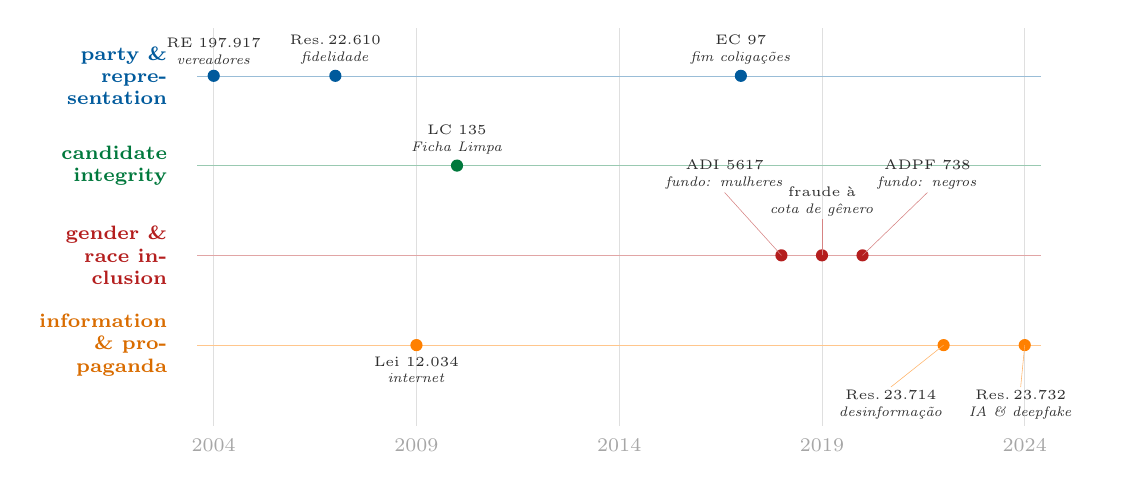
\begin{tikzpicture}[
    x=0.515cm, y=0.76cm,
    lane/.style={very thin},
    grid/.style={very thin, gray!25},
    lab/.style={font=\tiny, inner sep=1pt, align=center, text width=1.75cm, text=black!82},
    lanelab/.style={font=\scriptsize\bfseries, anchor=east, align=right, text width=1.7cm, inner sep=2pt},
    leader/.style={very thin},
  ]
  % year gridlines + axis labels
  \foreach \yr in {2004,2009,2014,2019,2024}{
     \pgfmathtruncatemacro\xx{\yr-2004}
     \draw[grid] (\xx,-1.35) -- (\xx,5.3);
     \node[font=\scriptsize, text=gray!70, anchor=north] at (\xx,-1.4) {\yr};
  }
  % lane guide rails + left labels (color = regulatory front)
  \draw[lane, myblue!40]  (-0.4,4.5) -- (20.4,4.5);
  \draw[lane, mygreen!40] (-0.4,3.0) -- (20.4,3.0);
  \draw[lane, myred!40]   (-0.4,1.5) -- (20.4,1.5);
  \draw[lane, orange!45]  (-0.4,0.0) -- (20.4,0.0);
  \node[lanelab, text=myblue]  at (-1.0,4.5) {party \& representation};
  \node[lanelab, text=mygreen] at (-1.0,3.0) {candidate integrity};
  \node[lanelab, text=myred]   at (-1.0,1.5) {gender \& race inclusion};
  \node[lanelab, text=orange!85!black] at (-1.0,0.0) {information \& propaganda};
  % ---- events: dot + label ----
  % party: 2004, 2007, 2017
  \fill[myblue] (0,4.5) circle (2.2pt);  \node[lab, anchor=south, yshift=3pt] at (0,4.5)  {RE 197.917\\\textit{vereadores}};
  \fill[myblue] (3,4.5) circle (2.2pt);  \node[lab, anchor=south, yshift=3pt] at (3,4.5)  {Res.\,22.610\\\textit{fidelidade}};
  \fill[myblue] (13,4.5) circle (2.2pt); \node[lab, anchor=south, yshift=3pt] at (13,4.5) {EC 97\\\textit{fim coliga\c{c}\~oes}};
  % integrity: 2010
  \fill[mygreen] (6,3.0) circle (2.2pt); \node[lab, anchor=south, yshift=3pt] at (6,3.0) {LC 135\\\textit{Ficha Limpa}};
  % inclusion: 2018, 2019, 2020 -- leaders fan out to avoid overlap
  \fill[myred] (14,1.5) circle (2.2pt); \draw[leader,myred!55] (14,1.5) -- (12.6,2.55); \node[lab, anchor=south] at (12.6,2.55) {ADI 5617\\\textit{fundo: mulheres}};
  \fill[myred] (15,1.5) circle (2.2pt); \draw[leader,myred!55] (15,1.5) -- (15.0,2.1);  \node[lab, anchor=south] at (15.0,2.1)  {fraude \`a\\\textit{cota de g\^enero}};
  \fill[myred] (16,1.5) circle (2.2pt); \draw[leader,myred!55] (16,1.5) -- (17.6,2.55); \node[lab, anchor=south] at (17.6,2.55) {ADPF 738\\\textit{fundo: negros}};
  % information: 2009, 2022, 2024
  \fill[orange] (5,0.0) circle (2.2pt);  \node[lab, anchor=north, yshift=-3pt] at (5,0.0)  {Lei 12.034\\\textit{internet}};
  \fill[orange] (18,0.0) circle (2.2pt); \draw[leader,orange!60] (18,0.0) -- (16.7,-0.7); \node[lab, anchor=north] at (16.7,-0.7) {Res.\,23.714\\\textit{desinforma\c{c}\~ao}};
  \fill[orange] (20,0.0) circle (2.2pt); \draw[leader,orange!60] (20,0.0) -- (19.9,-0.7); \node[lab, anchor=north] at (19.9,-0.7) {Res.\,23.732\\\textit{IA \& deepfake}};
\end{tikzpicture}
\end{center}
\vspace{-2pt}
{\centering\scriptsize\ns{The same arc appears in our caseload. Adversarial litigation recomposes across these fronts, with \emph{fraude \`a cota} up and propaganda down, rather than rising in aggregate.}\par}
\smallskip
\centerline{\hyperlink{app:recomp}{\beamergotobutton{Show it in the caseload}}\quad\hyperlink{src:motivation}{\beamerreturnbutton{Back}}}
\end{frame}

% ============================================================

\begin{frame}{Appendix --- Adjudication Geography and the Sample}
\hypertarget{app:geography}{}
\begin{columns}[T]

\begin{column}{0.60\textwidth}
  \vspace{-4pt}
  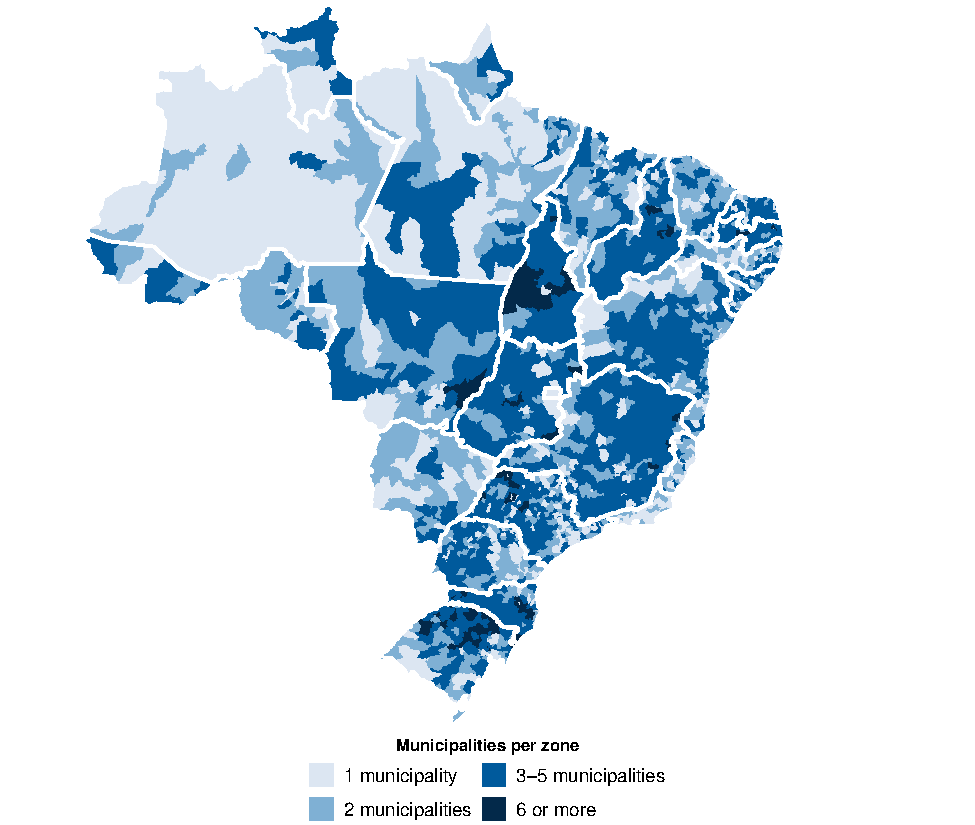
\includegraphics[width=\linewidth,height=0.55\textheight,keepaspectratio]{../figures/sample_map.pdf}
\end{column}

\begin{column}{0.38\textwidth}
  \vspace{4pt}
  \textbf{Adjudication geography}
  \smallskip

  \footnotesize
  \renewcommand{\arraystretch}{1.05}
  \begin{tabular}{lr}
    \toprule
    & \\[-6pt]
    Municipalities & \NMunisUniverse \\
    Electoral zones & \NZonesUniverse \\
    States (UF) & \NStatesUniverse \\
    Avg.\ munis per zone & \AvgMunisPerZone \\
    \bottomrule
  \end{tabular}

  \medskip
  \textbf{Zone size distribution}
  \smallskip

  \begin{tabular}{lrr}
    \toprule
    Munis per zone & Zones & Share \\
    \midrule
    1 & \ZoneDistOneN & \ZoneDistOnePct\% \\
    2 & \ZoneDistTwoN & \ZoneDistTwoPct\% \\
    3--5 & \ZoneDistThreeFiveN & \ZoneDistThreeFivePct\% \\
    6 or more & \ZoneDistSixN & \ZoneDistSixPct\% \\
    \bottomrule
  \end{tabular}

\end{column}

\end{columns}
\vspace{2pt}
\scriptsize
First-instance electoral cases are decided in the \emph{zona eleitoral} (\emph{ju\'izo eleitoral}), presided by a state judge. Each zone sits under one state electoral court (TRE), whose rulings bind every zone in the state, and the TSE sits above all. The decision locus is a three-tier hierarchy (zone $\subset$ state/TRE $\subset$ nation/TSE), and shocks to jurisprudence and enforcement diffuse down it. A zone holds \AvgMunisPerZone{} municipalities on average, many spanning several (table). We read each lawsuit's \textbf{munic\'ipio de origem} from the TSE SIG export (IBGE-matched for 99.99\% of filings) and analyze at the municipality level, while the adjudicating unit above it remains the \textbf{state/TRE}.\hfill\hyperlink{src:ejustice}{\beamerreturnbutton{Back}}
\end{frame}


\begin{frame}{Appendix --- The Analysis Sample}
\hypertarget{app:sample}{}
\footnotesize
The panel covers \NMunisUniverse{} Brazilian municipalities; the estimation sample, with complete controls and 2016 baselines, is $N=$~\NMunis{}. The table describes 2020$\to$2024 changes, while the estimator conditions the 2024 level on its 2016 baseline.
\vspace{-4pt}
\begin{center}
\scriptsize
\resizebox{\linewidth}{!}{% Auto-generated by code/04_analysis/09_summary_statistics.R
% Do not edit manually -- rerun the generating script to update

\begin{tabular}{lcccccc}
\toprule\toprule
 & $N$ & Mean & SD & P10 & Median & P90 \\
\midrule
\multicolumn{7}{l}{\textit{Litigation and the instrument}} \\
Adversarial lawsuits, 2020 (count) & 5,571 & 8.5 & 24.2 & 0.0 & 3.0 & 18.0 \\
Treatment: $\Delta\log(1+\text{lawsuits})$, 2020--2024 & 5,571 & -0.075 & 0.973 & -1.386 & 0.000 & 1.099 \\
Instrument: shift-share exposure ($Z_m$) & 5,571 & -0.252 & 0.352 & -0.607 & -0.219 & 0.000 \\
\midrule
\multicolumn{7}{l}{\textit{Mayoral electoral outcomes (2024 $-$ 2020 change)}} \\
Winner$-$runner-up margin & 5,569 & 0.060 & 0.325 & -0.293 & 0.043 & 0.458 \\
Runner-up vote share & 5,569 & -0.011 & 0.159 & -0.203 & -0.009 & 0.167 \\
Effective number of candidates & 5,569 & -0.237 & 0.791 & -1.165 & -0.109 & 0.678 \\
Blank-vote rate & 5,568 & 0.001 & 0.025 & -0.008 & -0.001 & 0.008 \\
Null-vote rate & 5,568 & -0.006 & 0.032 & -0.019 & -0.007 & 0.005 \\
Valid-vote rate & 5,568 & 0.015 & 0.065 & -0.032 & 0.014 & 0.071 \\
\midrule
\multicolumn{7}{l}{\textit{Predetermined controls}} \\
Log population, 2010 & 5,560 & 9.414 & 1.148 & 8.061 & 9.300 & 10.883 \\
Urban share, 2010 & 5,560 & 0.638 & 0.220 & 0.329 & 0.646 & 0.927 \\
Log income per capita, 2010 & 5,560 & 6.231 & 0.472 & 5.602 & 6.288 & 6.823 \\
Higher-education share, 2010 & 5,560 & 0.055 & 0.032 & 0.023 & 0.048 & 0.096 \\
Victory margin, 2016 & 5,565 & 0.185 & 0.212 & 0.020 & 0.119 & 0.412 \\
\bottomrule\bottomrule
\end{tabular}
}
\end{center}
\end{frame}

\input{frames/app_recomp.tex}


% ---------------------------------------------------------------------------
% A3b -- pushes the "mandatory-dominated, no wave" shape back to a PRE-SAMPLE
% (2016) baseline from an INDEPENDENT source (TRE-SP SAC-JE), the only 2016
% litigation snapshot we have. Compatibility is deliberately loose: 2016 zone
% IDs (SAC-JE, 1-427) do not align with the SIG panel's zone-codes (1-107), so
% this is a STATE-LEVEL composition comparison, never zone-by-zone; source
% changes across the divide, so only within-source SHARES are read (no count
% trend). Numbers come from lawsuit_composition_sp.tex, generated by
% 04_analysis/08_lawsuit_composition_sp.py -- nothing hard-coded.
% ---------------------------------------------------------------------------
\begin{frame}{Appendix --- SP Litigation Composition, 2016--2024}
\hypertarget{app:sp2016}{}
\footnotesize
\noindent A separate TRE-SP filing extract (S\~{a}o Paulo, all 645 municipalities) gives the only \textbf{pre-2020} snapshot of the docket. It carries the flat, mandatory-dominated shape back to before the sample period. The mandatory core (candidacy registration and campaign accounts) is the overwhelming majority of filings in every cycle ($\sim$95\%, shaded rows), and the adversarial slice is small and rises only gently across the three cycles (shaded, bottom).
\smallskip
\begin{columns}[T]
\begin{column}{0.50\linewidth}
\centering
\resizebox{\linewidth}{!}{% Auto-generated by code/04_analysis/08_lawsuit_composition_sp.py
% Do not edit manually -- rerun the generating script to update

\begin{tabular}{lccc}
\toprule\toprule
 & \textbf{2016} & \textbf{2020} & \textbf{2024} \\
 & \scriptsize{TRE-SP} & \scriptsize{SIG} & \scriptsize{SIG} \\
\midrule
\multicolumn{4}{l}{\textit{Mandatory / ancillary filings}} \\
\quad Candidacy registration & 62.8 & 52.2 & 49.9 \\
\quad Campaign accounts & 32.1 & 42.7 & 44.0 \\
\rowcolor{mylight}
\textbf{Mandatory core} & \textbf{94.9} & \textbf{94.9} & \textbf{93.8} \\
\midrule
\multicolumn{4}{l}{\textit{Adversarial filings}} \\
\quad Representa\c{c}\~{a}o & 2.45 & 2.58 & 2.97 \\
\quad Propaganda$^{\dagger}$ & 0.00 & 0.67 & 1.01 \\
\quad AIJE / AIME / criminal & 0.44 & 0.31 & 0.27 \\
\rowcolor{mylight}
\textbf{Adversarial} & \textbf{2.89} & \textbf{3.57} & \textbf{4.25} \\
\midrule
Administrative \& other & 2.2 & 1.5 & 1.9 \\
\bottomrule\bottomrule
\end{tabular}
}
\end{column}
\begin{column}{0.48\linewidth}
{\scriptsize
The 2016 baseline does two kinds of work. It confirms that the mandatory-filing exclusion is structural rather than a 2020-era SIG artifact, since the $\sim$95\% core predates our data. It also extends the ``expanded role, not volume'' reading to a pre-sample year: against a clean 2016 benchmark the adversarial arena still does not expand sharply.\par
\smallskip
$^{\dagger}$\,The propaganda row requires care. In 2016 there was no dedicated propaganda class, and those complaints filed as \emph{Representa\c{c}\~{a}o}, so the apparent $0\to1\%$ rise is partly TSE reclassification rather than behavior. The total adversarial share is comparable across cycles; its internal split is not.\par}
\end{column}
\end{columns}
\smallskip
{\centering\scriptsize Only some comparisons are licensed here. Zone identifiers do not align across sources (2016 SAC-JE spans zones 1--427; the SIG panel carries codes 1--107), so this is a state-level composition comparison rather than a zone-by-zone one. The source also changes at the 2016/2020 divide, so only within-source shares are read, never a raw-count trend.\par}
\smallskip
\centerline{\hyperlink{app:recomp}{\beamerreturnbutton{Recomposition (2020--24)}}\quad\hyperlink{src:motivation}{\beamerreturnbutton{Back}}}
\end{frame}



\begin{frame}{Appendix --- How to Read the Coefficient $\tau$}
\hypertarget{app:readtau}{}
\small
The headline number in every table is $\tau$, the 2SLS coefficient on the \emph{instrumented} change in litigation. Three things fix its meaning:
\smallskip
\begin{itemize}\itemsep3pt
  \item The treatment is a log-change. $\Delta\log(1+\ell_m)$ is approximately the proportional growth in a municipality's adversarial caseload from 2020 to 2024. A one-unit rise multiplies litigation by $e$ ($\approx+170\%$), and a doubling of lawsuits is a rise of $\log 2 \approx 0.69$. So $\tau$ is the outcome change per unit of log-growth in litigation, and $0.69\,\tau$ is the change per doubling.
  \item The outcome is a 2024 level net of its 2016 baseline. Conditioning on the 2016 baseline makes $\tau$ the effect on where a municipality ends up in 2024, holding its 2016 starting point fixed, rather than the effect on a change score. Shares, rates and margins lie in $[0,1]$, so $\tau=0.092$ means $+9.2$ percentage points, to be compared with the ``Mean of dep.\ var.'' row.
  \item It is a LATE for onset compliers. 2SLS recovers the effect for municipalities whose litigation responds to the diffusing national shock, not an average over all \NMunis. The first stage is identified off the extensive margin, meaning whether a contest enters the judicial arena at all (see \hyperlink{app:extensive}{extensive-margin appendix}), so the compliers are municipalities crossing into adversarial contestation rather than those scaling up an existing caseload.
\end{itemize}
\smallskip
\footnotesize \emph{Worked example, top-two margin ($\tau=\MarginCoef$).} A municipality whose adversarial litigation doubled relative to another ends 2024 with a margin $0.69\times\MarginCoef\approx\MarginDoublePP$ percentage points wider, starting from the same 2016 margin, against a 2024 mean of \MarginMean. Equivalently, a one-unit rise in predicted exposure (the Bartik index) raises litigation growth by $\FSCoef$ of a log-unit (first stage), i.e.\ a $\approx\MarginRFperUnitPP$pp wider margin in reduced form.\hfill\hyperlink{src:spec}{\beamerreturnbutton{Back to spec}}
\end{frame}


\begin{frame}{Appendix --- Identification: Pure First-Difference Bracket}
\hypertarget{app:fd}{}
\small
The headline conditions the 2024 level on the 2016 baseline ($Y_{2024}\sim D + Y_{2016}$, $\lambda$ freely estimated). This appendix re-estimates the \emph{same} headline outcomes as a pure first difference ($\Delta Y \sim D$), which pins the persistence coefficient $\lambda=1$.
\smallskip
\begin{center}
\scriptsize
\resizebox{\linewidth}{!}{% Auto-generated by code/03_estimation/02_iv_main.R
% Do not edit manually -- rerun the generating script to update

\begin{tabular}{lcccccc}
   \tabularnewline \midrule \midrule
   Dependent Variables: & $\Delta$ Margin (W$-$RU)  & $\Delta$ Winner vote share  & $\Delta$ Runner-up vote share  & $\Delta$ Winner majority (P50)  & $\Delta$ Blank (mayoral)  & $\Delta$ Null (mayoral)\\   
   Model:               & (1)                       & (2)                         & (3)                            & (4)                             & (5)                       & (6)\\  
   Judicialization      & 0.028                     & 0.020                       & -0.008                         & 0.065                           & 0.0003                    & -0.002\\   
                        & (0.027)                   & (0.018)                     & (0.013)                        & (0.058)                         & (0.002)                   & (0.002)\\   
   2024 Mean            & 0.060                     & 0.048                       & -0.012                         & 0.124                           & 0.001                     & -0.006\\  
   \midrule \midrule
   \multicolumn{7}{l}{\emph{Clustered (state) standard-errors in parentheses}}\\
   \multicolumn{7}{l}{\emph{Signif. Codes: ***: 0.01, **: 0.05, *: 0.1}}\\
\end{tabular}
}
\end{center}
\smallskip
\footnotesize Municipal margins barely persist from one cross-section to the next, so forcing $\lambda=1$ over-differences the outcome: the consolidation and withdrawal coefficients collapse toward zero and lose significance. The contrast identifies freeing $\lambda$ as the appropriate estimator for a barely-persistent outcome rather than as a specification that manufactures the result. Dep.\ var.\ means are $\Delta$ means; state (UF) FE; SEs clustered by state. \hfill\hyperlink{src:fd}{\beamerreturnbutton{Back to spec}}
\end{frame}


\begin{frame}{Appendix --- Rotemberg Weights and Shock Concentration}
\hypertarget{app:rotemberg}{}
\footnotesize
\textcolor{myblue}{This is a Goldsmith--Pinkham (GPS) share-identified design rather than a many-shock design.} With only $K_{\text{eff}}=\KeffRotemberg$ effective shocks, credibility rests on the exogeneity of the 2020 shares rather than on averaging away many independent shifters \citep{goldsmith2020,borusyak2022}. The Rotemberg decomposition assigns each subject a weight $\alpha_k$, summing to one, for how much it drives the 2SLS estimate.
\smallskip
\begin{columns}[T]
\begin{column}{0.55\textwidth}
\centering\scriptsize
\renewcommand{\arraystretch}{1.25}
\begin{tabular}{lrr}
\toprule
\textbf{Highest-weight subject} & $\alpha_k$ (\%) & Own $F_k$ \\
\midrule
\RotNameOne   & \RotPctOne   & \RotFOne \\
\RotNameTwo   & \RotPctTwo   & \RotFTwo \\
\RotNameThree & \RotPctThree & \RotFThree \\
\RotNameFour  & \RotPctFour  & \RotFFour \\
\RotNameFive  & \RotPctFive  & \RotFFive \\
\midrule
\textit{Top five} & \textbf{\RotTopFiveCumPct} & --- \\
\bottomrule
\end{tabular}\\[3pt]
{\tiny All five are \emph{Propaganda Eleitoral} subjects.}
\end{column}
\begin{column}{0.43\textwidth}
\scriptsize
What identifies the estimate is propaganda diffusion. The five highest-weight subjects carry \RotTopFiveCumPct\% of the net weight and propaganda subjects \RotPropagandaPct\%, above propaganda's \RecPropShare\% share of the instrument's raw variation, because the Rotemberg weight measures leverage rather than volume. These subjects are not weak (own $F_k$ of \RotFOne, \RotFTwo, \ldots), so the concentration is not a weak-instrument artifact: a few national propaganda-regulation shocks, covering internet rules, timing and permitted media, do the identifying work.
\smallskip

This does not contradict the national decline in propaganda litigation, because identification uses leave-own-state-out variation in each topic's growth across states rather than that trend: a topic can shrink on average and still diffuse unevenly. The exclusion restriction must then hold for propaganda specifically; the share-exogeneity checks address pre-trends and generic litigiousness, and a national recode is taken up separately \hyperlink{app:reclass}{\beamergotobutton{coding artifact?}}.
\end{column}
\end{columns}
\footnotesize The concentration is intrinsic to litigation data rather than a modeling choice: a finer partition raises the shock count but destroys first-stage relevance. The design is therefore defended on share exogeneity.\hfill\hyperlink{src:identbrief}{\beamerreturnbutton{Back}}
\end{frame}



\begin{frame}{Appendix --- Share Exogeneity: Intensity Control and Placebo Shifter}
\hypertarget{app:shares}{}
\footnotesize
The exogenous-shares path requires that the 2020 exposure shares isolate the \emph{adversarial} channel rather than proxy a municipality's overall litigiousness. Two checks (full BHJ treatment):
\begin{itemize}\itemsep0pt
  \item \textbf{Intensity control.} Add the 2020 \emph{level} of non-adversarial filings as a pre-determined control. If the shares proxied generic litigation volume, conditioning on it would move the estimate. It does not (margin $\PlaceboMainCoef\!\to\!\PlaceboIntensCoef$).
  \item \textbf{Placebo shifter.} Build an identically-constructed Bartik from the excluded mandatory and administrative filings. Its reduced form is null (margin $\PlaceboRFCoef$, SE $\PlaceboRFSE$) and its own relevance near zero ($F=\PlaceboRelevanceF$), as a non-channel should be.
\end{itemize}
\vspace{-2pt}
\begin{center}
\scriptsize
\resizebox{!}{0.24\textheight}{% Auto-generated by code/03_estimation/04_placebo_nonadversarial.R
% Do not edit manually -- rerun the generating script to update

\begin{tabular}{lcccc}
\toprule
 & Main IV & + Non-adv. & + Placebo & Placebo \\
 & & intensity & Bartik ctrl & reduced form \\
\midrule
Margin (W$-$RU) & 0.062$^{*}$ & 0.062$^{*}$ & 0.061$^{*}$ & 0.064 \\
 & (0.023) & (0.023) & (0.023) & (0.088) \\[2pt]
Winner majority & 0.057 & 0.053 & 0.057 & 0.094 \\
 & (0.036) & (0.035) & (0.036) & (0.119) \\[2pt]
Runner-up share & -0.032$^{*}$ & -0.033$^{*}$ & -0.031$^{*}$ & -0.033 \\
 & (0.012) & (0.012) & (0.012) & (0.045) \\[2pt]
Female vote share & -0.026 & -0.026 & -0.026 & 0.060 \\
 & (0.020) & (0.020) & (0.020) & (0.094) \\[2pt]
Turnout rate & -0.002 & -0.002 & -0.002 & 0.010 \\
 & (0.004) & (0.004) & (0.004) & (0.012) \\[2pt]
Blank vote rate & 0.003$^{\dagger}$ & 0.003$^{\dagger}$ & 0.003$^{\dagger}$ & 0.003 \\
 & (0.002) & (0.002) & (0.002) & (0.008) \\[2pt]
\midrule
First-stage $F$ & 102.3 & & & \\
$N$ & 5,560 & & & \\
\bottomrule
\end{tabular}
}
\end{center}
\vspace{-2pt}
\footnotesize \emph{Columns:} main IV; $+$ non-adversarial intensity; $+$ placebo Bartik control; placebo reduced form. The main coefficient is unmoved by either, so the shares carry the adversarial signal.
\smallskip
\centerline{\hyperlink{src:identbrief}{\beamerreturnbutton{Back}}}
\end{frame}



\begin{frame}{Appendix --- Inference: Few Clusters and the Exposure-Robust Bound}
\hypertarget{app:inference}{}
\footnotesize
The point estimate is invariant to how standard errors are computed. What moves is precision, and with it the weak-IV verdict. We cluster at the state level, where the leave-own-state shift is constant.
\smallskip
\begin{itemize}\itemsep3pt
  \item \textbf{Why state.} The leave-own-state-out shifter is identical within a state, so state clustering is the conservative default. Residuals also correlate across units with similar shares wherever they are located \citep{adao2019}; the exposure-robust SE below addresses that.
  \item \textbf{Few clusters $\Rightarrow$ weak-IV-robust AR.} State clustering leaves only \textbf{\NClusters{} clusters}, where asymptotic cluster-robust SEs can under-cover. Headline inference is therefore carried by an Anderson--Rubin \textbf{wild-cluster restricted bootstrap} (\ns{\citealp{andersonrubin1949,roodman2019}}; $B=9999$, Rademacher weights over \ARNClusters{} states). It confirms the consolidation (margin $p=\ARMarginP$, runner-up share $p=\ARRunnerUpP$, both excluding zero), leaves the mayoral blank rate tentative (the AR set straddles zero, $p=\ARBlankP$), and leaves the null outcomes (turnout, winner-majority, female share) null.
  \item \textbf{Exposure-robust outer bound.} The BHJ/AKM standard error \ns{\citep{borusyak2022,adao2019}}, built for the few-shock shift-share structure and re-clustered at the subject (shock) level, inflates the headline margin SE by only $\ERMarginRatio\times$, so the consolidation still clears. The SE barely moves because the estimate does not hang on one dominant shock. \hfill\hyperlink{app:exposure}{\beamergotobutton{weak-IV \& exposure-robust appendix}}
\end{itemize}

\centerline{\hyperlink{src:identbrief}{\beamerreturnbutton{Back}}}
\end{frame}



\begin{frame}{Appendix --- Weak-IV and Exposure-Robust Inference}
\hypertarget{app:exposure}{}
\small
The headline uses conventional state-clustered standard errors. Two stress tests bracket that choice, one addressing weak instruments and one the few-shock shift-share structure.
\smallskip

\textbf{(a) Anderson--Rubin wild-cluster restricted bootstrap} (\ARNClusters{} state clusters). It inverts the AR statistic and is valid regardless of instrument strength.
\begin{center}\scriptsize\renewcommand{\arraystretch}{1.15}
\begin{tabular}{lcc}
\toprule
Outcome & AR 95\% CI & $p$ \\
\midrule
Top-two margin        & \ARMarginCI   & \ARMarginP \\
Runner-up vote share  & \ARRunnerUpCI & \ARRunnerUpP \\
Mayoral blank rate    & \ARBlankCI    & \ARBlankP \\
Turnout (placebo)     & \ARTurnoutCI  & \ARTurnoutP \\
Female vote share     & \ARFemaleVSCI & \ARFemaleVSP \\
\bottomrule
\end{tabular}
\end{center}
\scriptsize The consolidation (margin, runner-up) clears. The blank-rate confidence interval straddles zero, which is why the withdrawal reading is carried as tentative. The compulsory-turnout placebo and the representation null are, as expected, indistinguishable from zero.
\smallskip

\textbf{(b) BHJ/AKM exposure-robust standard error}, the outer bound for a design identified off a handful of diffusing litigation topics. It re-clusters at the shock (subject) level.
\begin{center}\footnotesize
Top-two margin: conventional SE $\ERMarginSEconv \to$ exposure-robust $\ERMarginSEbhj$ (a $\ERMarginRatio\times$ inflation); $p=\ERMarginPbhj$; null-imposed CI $\ERMarginCI$ excludes zero.
\end{center}
\footnotesize The consolidation survives even under the most conservative shock-level clustering. The standard error barely moves because the estimate does not hang on a single dominant shock. \hfill\hyperlink{src:spine1}{\beamerreturnbutton{Back to the margin}}
\end{frame}


% ---------------------------------------------------------------------------
% Confronts the sharpest shift-share attack: with 20.6% of munis at zero 2020
% adversarial litigation, is the first stage (and the finding) just a
% zero-vs-any switch on the log1p floor? Honest split: Panel A concedes the
% RELEVANCE is extensive (intensive slope F=1.1) and confirms it is NOT a log1p
% artifact via count-native Poisson/NegBin (both null intensive); Panel B shows
% the OUTCOME is not extensive (margin RF survives dropping zeros + a horse race
% vs the presence dummy). Then reframed: the extensive margin IS the meaningful
% treatment -- the ONSET of adversarial contestation -- not a defect.
% Numbers from extensive_margin{,_macros}.tex, generated by 09_extensive_margin.R.
% ---------------------------------------------------------------------------
\begin{frame}{Appendix --- The Extensive Margin of the First Stage}
\hypertarget{app:extensive}{}
\footnotesize
\noindent \ExtMassPointPct\% of municipalities (\ExtMassPointN{}) have zero adversarial litigation in the 2020 base year, a mass point at the origin of $\Delta\log(1+\ell_m)$. The concern this raises is whether the first stage, and with it the finding, rides a crude zero-versus-any switch rather than the shift-share composition the construction claims.
\smallskip
\begin{columns}[T]
\begin{column}{0.53\linewidth}
\centering
\resizebox{\linewidth}{!}{% Auto-generated by code/03_estimation/09_extensive_margin.R -- do not edit.
\begin{tabular}{lccc}
\toprule\toprule
 & Coef. & (SE) & $F$ / $p$ \\
\midrule
\multicolumn{4}{l}{\textit{Panel A. First stage:} $\Delta\log(1+\ell_m)$} \\
Bartik $Z$ --- full ($N=5,560$) & 0.418$^{***}$ & \textcolor{mygray}{(0.041)} & $F=102$ \\
Bartik $Z$ --- litigating only ($N=4,414$) & 0.039 & \textcolor{mygray}{(0.037)} & $F=1.1$ \\
Presence $\mathbf{1}[\ell_{2020}>0]$ --- full & -1.024$^{***}$ & \textcolor{mygray}{(0.055)} & $F=342$ \\
\midrule
\multicolumn{4}{l}{\textit{Panel B. Reduced form: 2024 top-two margin}} \\
Bartik $Z$ --- full & 0.026$^{***}$ & \textcolor{mygray}{(0.008)} & $p=0.003$ \\
\rowcolor{mylight}
Bartik $Z$ --- litigating only & 0.021$^{**}$ & \textcolor{mygray}{(0.008)} & $p=0.022$ \\
\rowcolor{mylight}
Bartik $Z$ --- net of presence dummy & 0.023$^{***}$ & \textcolor{mygray}{(0.008)} & $p=0.009$ \\
Presence dummy --- net of $Z$ & -0.007 & \textcolor{mygray}{(0.009)} & $p=0.45$ \\
\bottomrule\bottomrule
\end{tabular}
}
\end{column}
\begin{column}{0.45\linewidth}
{\scriptsize
\textbf{Panel A: relevance is mostly extensive.} Among litigating municipalities only, the intensive slope collapses ($F=\ExtFSintensiveF$). The presence dummy alone is mechanically hyper-predictive, and its negative sign is the log1p floor, since a zero-litigation municipality can only grow. This is the convergence the first stage is identified off.\par
\textbf{This is not a log1p artifact.} A count model has no floor and returns the same verdict: modeling the caseload natively (Poisson and NegBin ANCOVA, zeros absorbed directly) leaves $Z$ with no proportional effect conditional on the 2020 baseline (PPML $p=\ExtPPMLfullP$, NegBin $p=\ExtNBfullP$, and null among litigators as well). The weak intensive margin is real.\par
\textbf{Panel B: the finding is not extensive.} The margin reduced form survives both dropping the entire zero mass point (litigating-only $p=\ExtRFpositiveP$) and a horse race against the presence dummy, where $Z$ stays significant ($p=\ExtRFhorseZP$) and presence is wrong-signed and null ($p=\ExtRFhorseDzeroP$). Only \ExtZonDzeroRtwo{} of $Z$'s variance is presence.\par}
\end{column}
\end{columns}
{\centering\scriptsize $Z$ predicts whether a contest enters the judicial arena rather than the caseload once it is in, and that onset of adversarial contestation is itself the expanded-role treatment. Since the outcome response is not a zero-versus-any jump (Panel B), 2SLS remains a clean LATE for these onset compliers. Only the per-unit-of-volume magnitude leans on the extensive first stage.\par}
\smallskip
\centerline{\hyperlink{src:firststage}{\beamerreturnbutton{First stage}}\quad\hyperlink{app:tdef}{\beamergotobutton{Does the log1p form drive it?}}\quad\hyperlink{src:spine1}{\beamerreturnbutton{Back to the margin}}}
\end{frame}


% ---------------------------------------------------------------------------
% Companion to app:extensive: is the finding an artifact of the log1p treatment
% definition? Re-estimates the headline margin 2SLS under 5 ways of measuring the
% litigation change, SAME Bartik Z. The teaching point: the reduced form (margin~Z)
% is ONE number invariant to the treatment transform, so only the units and the
% first-stage F move. Numbers from treatment_definition{,_macros}.tex (12_...R).
% ---------------------------------------------------------------------------
\begin{frame}{Appendix --- Sensitivity to the Treatment Definition}
\hypertarget{app:tdef}{}
\footnotesize
\noindent The endogenous variable is $\Delta\log(1+\ell)$. The $\log(1+\cdot)$ form is a modeling choice that compresses large counts and floors at zero, which raises the question of whether the consolidation survives other reasonable ways to measure the change in litigation. We re-estimate the headline ANCOVA-2016 margin 2SLS under \TdefNdefs{} treatment definitions, holding the same Bartik instrument, controls, state FE, and clustering fixed.
\smallskip
\begin{columns}[T]
\begin{column}{0.54\linewidth}
\centering
\resizebox{\linewidth}{!}{% Auto-generated by code/03_estimation/12_treatment_definition.R -- do not edit.
\begin{tabular}{lccccc}
\toprule\toprule
 & \multicolumn{2}{c}{First stage} & \multicolumn{3}{c}{2SLS: 2024 top-two margin} \\
\cmidrule(lr){2-3}\cmidrule(lr){4-6}
Treatment definition & Coef. & $F$ & Coef. & /\,SD & $p$ \\
\midrule
\rowcolor{mylight}
$\Delta\log(1+\ell)$ \;\scriptsize(baseline) & 0.418 & $102.3$ & 0.062$^{**}$ & 0.060 & $0.013$ \\
\rowcolor{mylight} & \textcolor{mygray}{(0.041)} & & \textcolor{mygray}{(0.023)} & & \\
$\Delta\,\mathrm{asinh}(\ell)$ & 0.536 & $104.2$ & 0.048$^{**}$ & 0.057 & $0.013$ \\
 & \textcolor{mygray}{(0.052)} & & \textcolor{mygray}{(0.018)} & & \\
$\Delta\ell$ \;\scriptsize(raw count) & 0.900 & $8.1$ & 0.029$^{*}$ & 0.534 & $0.074$ \\
 & \textcolor{mygray}{(0.316)} & & \textcolor{mygray}{(0.015)} & & \\
$\Delta\ell$ per 1{,}000 votes & 4.427 & $2.7$ & 0.006 & 0.389 & $0.163$ \\
 & \textcolor{mygray}{(2.695)} & & \textcolor{mygray}{(0.004)} & & \\
$\mathbf{1}[\ell_{24}{>}0]-\mathbf{1}[\ell_{20}{>}0]$ & 0.308 & $163.6$ & 0.084$^{***}$ & 0.041 & $0.006$ \\
 & \textcolor{mygray}{(0.024)} & & \textcolor{mygray}{(0.028)} & & \\
\bottomrule\bottomrule
\end{tabular}
}
\end{column}
\begin{column}{0.44\linewidth}
{\scriptsize
One fact organizes the table. The reduced form $\text{margin}\sim Z$ is a single number ($\TdefRFcoef$, $p=\TdefRFp$), invariant to how the treatment is transformed. Each 2SLS column is that fixed reduced form divided by a definition-specific first stage, so what moves across columns is the magnitude's units and the first-stage $F$, never the sign.\par
\smallskip
The instrument predicts the compressed treatments strongly (log1p, IHS, onset: $F$ up to \TdefFhi) and the raw-count magnitude weakly (levels, rate: $F$ as low as \TdefFlo). Where significance softens, then, it is a weak-instrument symptom of the raw-count first stage rather than counter-evidence, and it reflects the same extensive-margin fact documented in the preceding appendix. The per-1-SD effect stays positive throughout.\par}
\end{column}
\end{columns}
\smallskip
{\centering\scriptsize The sign is positive under all \TdefNdefs{} definitions; significance at 5\% holds under the three with strong first stages and not under levels ($p=\TdefLevelsP$) or the rate ($p=\TdefRateP$). The per-unit magnitude is definition-dependent, as \citet{chen2024} show for log-like transforms of outcomes with zeros. That is why the reduced form, rather than a units-laden 2SLS coefficient, is the object we treat as the headline.\par}
\smallskip
\centerline{\hyperlink{app:extensive}{\beamerreturnbutton{Extensive margin}}\quad\hyperlink{app:reclass}{\beamergotobutton{Is the shifter a coding artifact?}}\quad\hyperlink{src:spine1}{\beamerreturnbutton{Back to the margin}}}
\end{frame}


% ---------------------------------------------------------------------------
% Confronts topic-reclassification of the SHIFTER (assunto codes changing between
% 2020 and 2024). Honest, partly-uncomfortable frame: the instrument is 71%
% propaganda national shift (negative). Family-level Z (immune to within-family
% recode) keeps F=177, margin RF p=0.079; dropping propaganda entirely collapses
% the first stage (F=2.0) -- so identification rests on the propaganda decline being
% BEHAVIORAL (regime substitution: litigation -> takedowns), which is the thesis.
% Numbers from reclassification_robustness{,_macros}.tex (13_...R).
% ---------------------------------------------------------------------------
\begin{frame}{Appendix --- Topic Reclassification and the Shifter}
\hypertarget{app:reclass}{}
\footnotesize
\noindent The shifts are leave-own-state-out national growth rates of each \emph{assunto} (subject) code. A national recode between 2020 and 2024 would make a subject's growth spurious, and leave-own-state-out cannot absorb it, because such a recode hits every state at once. The exposure is concrete: \RecPropShare\% of the instrument's variation is the propaganda national shift, that shift is negative ($\RecPropShock$), and propaganda is the topic with documented recoding.
\smallskip
\begin{columns}[T]
\begin{column}{0.55\linewidth}
\centering
\resizebox{\linewidth}{!}{% Auto-generated by code/03_estimation/13_reclassification_robustness.R -- do not edit.
\begin{tabular}{lcccc}
\toprule\toprule
 & First stage & \multicolumn{3}{c}{Reduced form: 2024 margin} \\
\cmidrule(lr){2-2}\cmidrule(lr){3-5}
Instrument built at & $F$ & Coef. & (SE) & $p$ \\
\midrule
\rowcolor{mylight}
Subject-level \;\scriptsize(committed) & $102$ & 0.026$^{***}$ & \textcolor{mygray}{(0.008)} & $0.003$ \\
Topic-family \;\scriptsize(within-family recode immune) & $177$ & 0.052$^{*}$ & \textcolor{mygray}{(0.029)} & $0.079$ \\
Drop propaganda shift & $2$ & 0.031$^{**}$ & \textcolor{mygray}{(0.011)} & $0.011$ \\
\bottomrule\bottomrule
\end{tabular}
}
\end{column}
\begin{column}{0.43\linewidth}
{\scriptsize
The unit of the shifter is the subject, not the procedural vehicle: it is built on the \emph{assunto} rather than the \emph{classe}, so the documented propaganda$\leftrightarrow$Representa\c{c}\~ao recode, a vehicle relabeling, does not move its units.\par
\smallskip
Within-family recoding is not the explanation either. Rebuilding the instrument at the topic-family level makes it immune to reshuffling among subjects inside a family: the first stage stays strong ($F=\RecFamF$) and the margin reduced form positive ($\RecFamRFcoef$), softening to $p=\RecFamRFp$.\par
\smallskip
The limit is worth stating plainly. Dropping propaganda's shift entirely collapses the first stage ($F=\RecNoPropF$): the instrument is the propaganda decline. Identification therefore rests on that decline being behavioral, and the 2020--2024 fall in propaganda litigation is the documented substitution of case-by-case suits by administrative and platform takedown orders. That change in the arena's mode of operation is the expanded role this paper studies.\par}
\end{column}
\end{columns}
\smallskip
\centerline{\hyperlink{app:tdef}{\beamerreturnbutton{Treatment definition}}\quad\hyperlink{src:firststage}{\beamerreturnbutton{First stage}}\quad\hyperlink{src:spine1}{\beamerreturnbutton{Back to the margin}}}
\end{frame}


\begin{frame}{Appendix --- Many Outcomes, No Family Cut}
\hypertarget{app:multiplicity}{}
\footnotesize
The consolidation rests on a family of correlated outcomes, raising the question of whether it survives multiple-testing correction. We answer it without declaring which outcomes ``count,'' by two complementary routes.
\vspace{-2pt}

\begin{columns}[T]
\begin{column}{0.52\linewidth}
\scriptsize \textbf{(a) Collapse each theory-declared family to one index} (Anderson 2008 inverse-covariance / Kling--Liebman--Katz average). One family $=$ one test. Each 2024 index is net of its own 2016 baseline; effects in SD units, positive $=$ consolidation.
\vspace{-4pt}
\begin{center}
\scriptsize
\scalebox{0.95}{\resizebox{\linewidth}{!}{% Auto-generated by code/03_estimation/11_summary_indices.R
% Do not edit manually -- rerun the generating script to update

\begin{tabular}{lcccc}
\toprule\toprule
Family (\# outcomes) & Index effect & Std.\ error & $p$ & $N$ \\
\midrule
Closeness (mayoral) (4) & 0.219$^{***}$ & \textcolor{mygray}{(0.078)} & 0.009 & 5,560 \\
Field concentration (4) & 0.069 & \textcolor{mygray}{(0.067)} & 0.309 & 5,560 \\
Voter disengagement (4) & 0.143 & \textcolor{mygray}{(0.092)} & 0.134 & 5,560 \\
\midrule
\rowcolor{mylight}
Overall combined index (12) & 0.144$^{**}$ & \textcolor{mygray}{(0.066)} & 0.039 & 5,560 \\
\midrule
Descriptive representation (6) & 0.040 & \textcolor{mygray}{(0.045)} & 0.379 & 5,560 \\
Council ballot (placebo) (3) & 0.083 & \textcolor{mygray}{(0.097)} & 0.402 & 5,560 \\
\bottomrule\bottomrule
\end{tabular}
}}
\end{center}
\scriptsize The overall combined index clears ($p<.05$) and closeness clears on its own, while representation and the council-ballot placebo are null. The index pools 8 of 12 non-ballot outcomes, and the ballot family alone is $p=.134$, so it establishes the consolidation rather than a face.
\end{column}
\begin{column}{0.46\linewidth}
\scriptsize \textbf{(b) Romano--Wolf stepdown} over all 18 barrier/representation reduced forms, a \emph{joint} wild-cluster bootstrap ($B=10{,}000$, shared Rademacher weights) controlling the family-wise error rate.
\vspace{-4pt}
\begin{center}
\scriptsize
\scalebox{0.95}{\resizebox{\linewidth}{!}{% Auto-generated by code/03_estimation/11_summary_indices.R -- do not edit
\begin{tabular}{lcccc}
\toprule\toprule
Outcome & $t$ & $p_{\text{raw}}$ & $p_{\text{Holm}}$ & $p_{\text{RW}}$ \\
\midrule
Top-two margin & 3.35 & 0.001$^{***}$ & 0.015 & 0.059$^{*}$ \\
Runner-up vote share & -3.22 & 0.001$^{***}$ & 0.022 & 0.071$^{*}$ \\
Winner vote share & 2.75 & 0.006$^{***}$ & 0.094 & 0.160 \\
Vote Herfindahl & 1.96 & 0.050$^{*}$ & 0.751 & 0.559 \\
Mayoral blank rate & 1.95 & 0.051$^{*}$ & 0.751 & 0.559 \\
Mayoral null rate & 1.77 & 0.077$^{*}$ & 1.000 & 0.668 \\
\bottomrule\bottomrule
\end{tabular}
}}
\end{center}
\scriptsize Margin and runner-up survive raw and Holm correction. At the fully simultaneous family-wise level, which also carries the few-cluster penalty, they land borderline ($p_{\text{RW}}\!\approx\!.06$). Romano--Wolf is stricter than normal-approximation Holm because the bootstrap captures the \ARNClusters{}-cluster tails that the index averages over.
\end{column}
\end{columns}
\vspace{-4pt}
\footnotesize What the two routes establish is a pattern rather than a single star. The index, which requires no family cut, clears; the most heavily corrected coefficient is borderline, which is what \ARNClusters{} clusters buy. \ns{The family is fixed at these 18: the gender decomposition \hyperlink{src:gender}{\beamergotobutton{gender}} splits an outcome already inside it and is never counted as a new confirmatory test.} \hfill\hyperlink{src:spine1}{\beamerreturnbutton{Back to the margin}}
\end{frame}


\begin{frame}{Appendix --- Pre-Trend Placebo (consolidation ladder, numeric)}
\hypertarget{app:pretrend}{}
\small
The numeric placebo behind the balance coefplot: the 2016$\to$2020 pre-period change in each consolidation outcome, regressed on the instrumented 2020$\to$2024 treatment. A future shock cannot cause a past change, so a clean design returns coefficients near zero. Conditioned on pre-determined (2010 Census) covariates only; state FE; state-clustered.
\smallskip
\begin{center}
\scriptsize
\resizebox{\linewidth}{!}{% Auto-generated by code/03_estimation/02_iv_main.R
% Do not edit manually -- rerun the generating script to update

\begin{tabular}{l*{4}{c}}
\toprule\toprule
Dep.\ var.: & \textbf{Margin (W$-$RU)} & \textbf{Eff.\ N candidates} & \textbf{Vote HHI} & \textbf{Top-2 vote share} \\
\midrule
\rowcolor{mylight}
\textbf{Placebo (judicialization)} & 0.003 & -0.035 & 0.013 & 0.011 \\
\rowcolor{mylight}
 & \textcolor{mygray}{(0.038)} & \textcolor{mygray}{(0.070)} & \textcolor{mygray}{(0.018)} & \textcolor{mygray}{(0.012)} \\
\midrule
$N$ & 5,560 & 5,560 & 5,560 & 5,560 \\
Pre-trend mean & 0.017 & 0.087 & -0.011 & -0.022 \\
\bottomrule\bottomrule
\end{tabular}
}
\end{center}
\smallskip
\footnotesize Every rung is clean: margin ($\PtMarginCoef$, $p=\PtMarginP$), effective-N ($\PtEffNCoef$, $p=\PtEffNP$), Herfindahl ($\PtHHICoef$, $p=\PtHHIP$), top-two share ($\PtTopTwoCoef$, $p=\PtTopTwoP$). This differs from an earlier draft because that version conditioned the balance test on \texttt{margin\_2016}, the ladder's own 2016 baseline, which induced a regression-to-the-mean (Lord's paradox) artifact that read as a pre-trend. The baseline is inadmissible when the outcome is itself a 2016-based change, and dropping it clears every rung. \hfill\hyperlink{src:pretrend}{\beamerreturnbutton{Back to balance test}}
\end{frame}


\begin{frame}{Appendix --- Consolidation Robust to the Full Pre-Treatment Path}
\hypertarget{app:ptrobust}{}
\small
The balance test clears the margin, effective-N and top-two share, with the Herfindahl borderline. As a further check we add the 2020 base-year level to the headline 2016 lag, so the two lags $\{2016, 2020\}$ span both where a municipality started and the pre-slope it was on. The 2020 level is pre-determined with respect to the 2020$\to$2024 shock, since the instrument's shares are dated 2020 and the shifter leaves the own state out, so it is a legitimate control. The coefficient is then identified off the 2024 deviation from each municipality's own path.
\smallskip
\begin{center}
\scriptsize
\resizebox{\linewidth}{!}{% Auto-generated by code/03_estimation/02_iv_main.R
% Do not edit manually -- rerun the generating script to update

\begin{tabular}{l*{4}{c}}
\toprule\toprule
Dep.\ var.: & \textbf{$\Delta$ Margin (W$-$RU)} & \textbf{$\Delta$ Eff.\ N candidates} & \textbf{$\Delta$ Vote HHI} & \textbf{$\Delta$ Top-2 vote share} \\
\midrule
\rowcolor{mylight}
\textbf{Judicialization} & 0.057$^{**}$ & -0.044 & 0.022 & 0.001 \\
\rowcolor{mylight}
 & \textcolor{mygray}{(0.025)} & \textcolor{mygray}{(0.040)} & \textcolor{mygray}{(0.013)} & \textcolor{mygray}{(0.009)} \\
\midrule
$N$ & 5,560 & 5,560 & 5,560 & 5,560 \\
2024 Mean & 0.270 & 2.021 & 0.527 & 0.945 \\
2016 Mean & 0.193 & 2.172 & 0.492 & 0.929 \\
\bottomrule\bottomrule
\end{tabular}
}
\end{center}
\smallskip
\footnotesize The estimates are essentially unchanged. The top-two margin moves from its headline value $\MarginCoef$ to $\PtRobMarginCoef$ ($p=\PtRobMarginP$), while effective-N and the Herfindahl shift only in the third decimal and remain imprecise, as in the headline. Conditioning on both the 2020 level and the pre-slope a municipality was on leaves the result intact, which places the consolidation as a response to the 2020$\to$2024 shock rather than the continuation of a pre-existing path. \hfill\hyperlink{src:pretrend}{\beamerreturnbutton{Back to balance test}}
\end{frame}


\begin{frame}{Appendix --- Whole-Field Concentration Measures}
\hypertarget{app:concentration}{}
\small
Beyond the top-two gap, three measures read concentration across the \emph{whole} field: the effective number of candidates (Laakso--Taagepera), the vote-share Herfindahl, and the combined top-two share. Same headline spec (2024 level on the 2016 baseline, state FE, clustered by state).
\smallskip
\begin{center}
\scriptsize
\resizebox{\linewidth}{!}{% Auto-generated by code/03_estimation/02_iv_main.R
% Do not edit manually -- rerun the generating script to update

\begin{tabular}{l*{3}{c}}
\toprule\toprule
Dep.\ var.: & \textbf{$\Delta$ Eff.\ N candidates} & \textbf{$\Delta$ Vote HHI} & \textbf{$\Delta$ Top-2 vote share} \\
\midrule
\rowcolor{mylight}
\textbf{Judicialization} & -0.111$^{**}$ & 0.043$^{***}$ & 0.004 \\
\rowcolor{mylight}
 & \textcolor{mygray}{(0.046)} & \textcolor{mygray}{(0.014)} & \textcolor{mygray}{(0.009)} \\
\midrule
$N$ & 5,560 & 5,560 & 5,560 \\
2024 Mean & 2.021 & 0.527 & 0.945 \\
2016 Mean & 2.172 & 0.492 & 0.929 \\
\bottomrule\bottomrule
\end{tabular}
}
\end{center}
\smallskip
\footnotesize The Herfindahl rises ($\HHICoef$, $p=\HHIP$, significant at 10\%) and effective-N moves the consolidating way ($\EffNCoef$) though imprecisely ($p=\EffNP$), while the combined top-two share is flat ($\TopTwoCoef$, $p=\TopTwoP$). The three agree in direction, and the flat top-two share locates the redistribution within the leading pair, from runner-up to winner, rather than in two parties crowding out the rest of the field. The top-two margin carries the statistical weight, so these measures corroborate it without confirming it independently. \hfill\hyperlink{src:spine1}{\beamerreturnbutton{Back to the margin}}
\end{frame}


\begin{frame}{Appendix --- Binary and Raw-Count Closeness Outcomes}
\hypertarget{app:compbinary}{}
\small
Two mayoral closeness outcomes kept off the main top-two margin table. The winner-majority indicator (whether the winner cleared 50\% of valid votes) is the underpowered binary discretization of the continuous margin, and the log candidate count is the raw-count analog of the effective number of candidates already in the concentration measures. Same baseline specification (2024 value on the 2016 level, state FE, state-clustered).
\smallskip
\begin{center}
\scriptsize
\resizebox{0.6\linewidth}{!}{% Auto-generated by code/03_estimation/02_iv_main.R
% Do not edit manually -- rerun the generating script to update

\begin{tabular}{l*{2}{c}}
\toprule\toprule
Dep.\ var.: & \textbf{$\Delta$ Winner majority (P50)} & \textbf{$\Delta$ Log n candidates} \\
\midrule
\rowcolor{mylight}
\textbf{Judicialization} & 0.036 & -0.046$^{*}$ \\
\rowcolor{mylight}
 & \textcolor{mygray}{(0.036)} & \textcolor{mygray}{(0.027)} \\
\midrule
$N$ & 5,560 & 5,560 \\
2024 Mean & 0.832 & 1.268 \\
2016 Mean & 0.767 & 1.289 \\
\bottomrule\bottomrule
\end{tabular}
}
\end{center}
\smallskip
\footnotesize Both carry the consolidation sign, winner-majority positive and log-count negative (fewer candidates), and neither clears significance: winner majority $p=\WinMajP$, log count $p=\CandExecP$. The continuous top-two margin and the effective-N count are the better-powered measurements of the same quantity. \hfill\hyperlink{src:spine1}{\beamerreturnbutton{Back to the margin}}
\end{frame}


\begin{frame}{Appendix --- Campaign-Spending Attrition}
\hypertarget{app:spending}{}
\hypertarget{src:mechanism}{}
\small
The resource-attrition account holds that litigation drains a challenger's campaign funds faster than the front-runner's, tilting the contest before a vote is cast. We test it with a 2SLS of judicialization on the 2020$\to$2024 change in TSE campaign spending (SPCE contracted expenses), cut by vote rank (front-runner versus challenger) and by seat type. Attrition predicts that the challenger's spending, and their share of the top two, falls under exposure, most sharply where an incumbent is defended. Baseline controls; state FE; state-clustered; first stage $F=\FinFCont$ in contested seats, \FinFOpen{} in open seats and \FinFFull{} on all seats.
\smallskip
\begin{center}
\scriptsize
\resizebox{\linewidth}{!}{% Auto-generated by code/03_estimation/10_mechanism_finance.R
% Do not edit manually -- rerun the generating script to update

\begin{tabular}{l*{3}{c}}
\toprule\toprule
Subsample ($N$) & \textbf{$\Delta$ Log challenger spend} & \textbf{$\Delta$ Log front-runner spend} & \textbf{$\Delta$ Challenger spend share} \\
\midrule
\textbf{All seats} (5,560) & 0.086 & 0.102 & -0.027 \\
 & \textcolor{mygray}{(0.320)} & \textcolor{mygray}{(0.114)} & \textcolor{mygray}{(0.032)} \\
\textbf{Open seat} (2,026) & 0.285 & 0.100 & -0.023 \\
 & \textcolor{mygray}{(0.381)} & \textcolor{mygray}{(0.129)} & \textcolor{mygray}{(0.047)} \\
\rowcolor{mylight}
\textbf{Contested} (3,534) & -0.136 & 0.100 & -0.035 \\
\rowcolor{mylight}
 & \textcolor{mygray}{(0.379)} & \textcolor{mygray}{(0.141)} & \textcolor{mygray}{(0.028)} \\
\bottomrule\bottomrule
\end{tabular}
}
\end{center}
\smallskip
\footnotesize The evidence for attrition is suggestive at most. On the full sample every spending outcome is null, and in contested seats the signs line up (the challenger's spending falls, the front-runner's holds, the challenger's top-two share slips) but stay far from significant (best $p=\FinBestContP$). The channel we can measure is therefore voter withdrawal in these same contested seats \hyperlink{src:voterballot}{\beamergotobutton{ballot response}} rather than campaign finance: soft challenger support blanks out instead of being out-financed. \hfill\hyperlink{app:seatdisengage}{\beamerreturnbutton{Back}}
\end{frame}


\begin{frame}{Appendix --- Descriptive Representation (full table)}
\hypertarget{app:representation}{}
\small
Full 2SLS estimates underlying the coefficient plot: vote-weighted female and non-white share, the new/incumbent split, and winner identity. Outcome is the 2024 value, controlling for the 2016 level; state FE; SEs clustered by state.
\smallskip
\begin{center}
\scriptsize
\resizebox{\linewidth}{!}{% Auto-generated by code/03_estimation/02_iv_main.R
% Do not edit manually -- rerun the generating script to update

\begin{tabular}{lcccccc}
   \tabularnewline \midrule \midrule
   Dependent Variables: & Female vote share & Nonwhite vote share & $\Delta$ New-cand.\ vote share   & $\Delta$ Incumbent vote share  & Winner is female & $\Delta$ Winner is new entrant\\   
   Model:               & (1)               & (2)                 & (3)                              & (4)                            & (5)              & (6)\\  
   Judicialization      & -0.045            & -0.030              & -0.027                           & 0.039                          & -0.040           & 0.002\\   
                        & (0.029)           & (0.039)             & (0.037)                          & (0.042)                        & (0.044)          & (0.050)\\   
   2024 Mean            & 0.146             & 0.341               & 0.550                            & 0.315                          & 0.132            & 0.474\\  
   2016 Mean            & 0.128             & 0.303               &                                  &                                & 0.116            & \\  
   \midrule \midrule
   \multicolumn{7}{l}{\emph{Clustered (state) standard-errors in parentheses}}\\
   \multicolumn{7}{l}{\emph{Signif. Codes: ***: 0.01, **: 0.05, *: 0.1}}\\
\end{tabular}
}
\end{center}
\smallskip
\footnotesize \hfill\hyperlink{src:representation}{\beamerreturnbutton{Back to figure}}
\end{frame}


\begin{frame}{Appendix --- Gender Incidence: How the Split Is Built}
\hypertarget{app:gender}{}
\scriptsize
The outcome is constructed as $\text{female\_winner\_share} = \text{winner\_share} \times \mathbf{1}[\text{winner is female}]$, set to zero rather than missing when the winner is a man, and symmetrically for male winners and for the runner-up's slot. Two properties follow. \textbf{(i)} Female $+$ male equals the total exactly ($0.080+0.527=0.607$ for the winner and $0.057+0.280=0.337$ for the runner-up, the shares on \hyperlink{src:spine1}{\beamergotobutton{the headline}}), with $N=\NMunis$ in every column, so these columns decompose the headline rather than defining a new sample. \textbf{(ii)} Nothing is conditioned on. The tempting alternative, the mean share among races where a woman placed second, selects on an outcome of the same shock. The price of the unconditional construction is that each component mixes an extensive margin (how often a woman holds the slot, isolated by ``runner-up is female'') with an intensive one, so the pair is read together.

\medskip
\textbf{(a) Decomposition.} Female $+$ male reproduce the winner and runner-up totals column by column.
\begin{center}
\resizebox{\linewidth}{!}{% Auto-generated by code/03_estimation/02_iv_main.R
% Do not edit manually -- rerun the generating script to update

\begin{tabular}{l*{4}{c}}
\toprule\toprule
Dep.\ var.: & \textbf{$\Delta$ Female winner share} & \textbf{$\Delta$ Male winner share} & \textbf{$\Delta$ Female runner-up share} & \textbf{$\Delta$ Male runner-up share} \\
\midrule
\rowcolor{mylight}
\textbf{Judicialization} & -0.009 & 0.039$^{**}$ & -0.016 & -0.015 \\
\rowcolor{mylight}
 & \textcolor{mygray}{(0.015)} & \textcolor{mygray}{(0.018)} & \textcolor{mygray}{(0.011)} & \textcolor{mygray}{(0.014)} \\
\midrule
$N$ & 5,560 & 5,560 & 5,560 & 5,560 \\
2024 Mean & 0.080 & 0.527 & 0.057 & 0.280 \\
2016 Mean & 0.064 & 0.498 & 0.055 & 0.314 \\
\bottomrule\bottomrule
\end{tabular}
}
\end{center}
\medskip
\footnotesize \hyperlink{app:gendergap}{\beamergotobutton{(b) the differential tests}}\hfill\hyperlink{src:gender}{\beamerreturnbutton{Back to the gender split}}
\end{frame}


\begin{frame}{Appendix --- Gender Incidence: the Differential Tests}
\hypertarget{app:gendergap}{}
\scriptsize
The female$-$male gap in each slot is estimated as its own outcome rather than inferred from the two component columns. Reading a gendered effect off the contrast between a starred male component in (a) and an unstarred female one would be the difference-in-significance fallacy, since two estimates can sit on opposite sides of a significance threshold while the difference between them is nowhere near significant. That is what happens here: the male winner's gain clears at 5\% and the female winner's does not, yet the gap between them carries $p=\WinGapP$. The runner-up slot's gap, by contrast, is a precisely estimated zero ($\RUGapCoef$, SE $\RUGapSE$), which is a positive finding rather than an absence of one.

\medskip
\textbf{(b) Differential tests.}
\begin{center}
\resizebox{\linewidth}{!}{% Auto-generated by code/03_estimation/02_iv_main.R
% Do not edit manually -- rerun the generating script to update

\begin{tabular}{l*{4}{c}}
\toprule\toprule
Dep.\ var.: & \textbf{$\Delta$ Gap, winner's slot} & \textbf{$\Delta$ Gap, runner-up's slot} & \textbf{$\Delta$ Female top-2 share} & \textbf{$\Delta$ Runner-up is female} \\
\midrule
\rowcolor{mylight}
\textbf{Judicialization} & -0.048 & -0.001 & -0.025 & -0.031 \\
\rowcolor{mylight}
 & \textcolor{mygray}{(0.031)} & \textcolor{mygray}{(0.022)} & \textcolor{mygray}{(0.020)} & \textcolor{mygray}{(0.028)} \\
\midrule
$N$ & 5,560 & 5,560 & 5,560 & 5,560 \\
2024 Mean & -0.447 & -0.223 & 0.137 & 0.164 \\
2016 Mean & -0.434 & -0.259 & 0.118 & 0.142 \\
\bottomrule\bottomrule
\end{tabular}
}
\end{center}
\medskip
\footnotesize The last two columns give the net and extensive-margin readings: women's share of the top two, and how often the runner-up slot is held by a woman.
\hfill\hyperlink{app:gender}{\beamerreturnbutton{Back to (a)}}\,\hyperlink{src:gender}{\beamerreturnbutton{Back to the gender split}}
\end{frame}


\begin{frame}{Appendix --- The Council Race as Placebo Office}
\hypertarget{app:councilplacebo}{}
\small
The same instrument, built once from the executive design and applied to the council (vereador) race, returns a near-complete null: a large, fluid, multi-seat proportional contest absorbs the same litigation with almost no compositional trace. The asymmetry is what front-runner reinforcement predicts, since the mechanism operates on a single-winner race and has no counterpart in a multi-seat proportional one.
\smallskip
\begin{center}
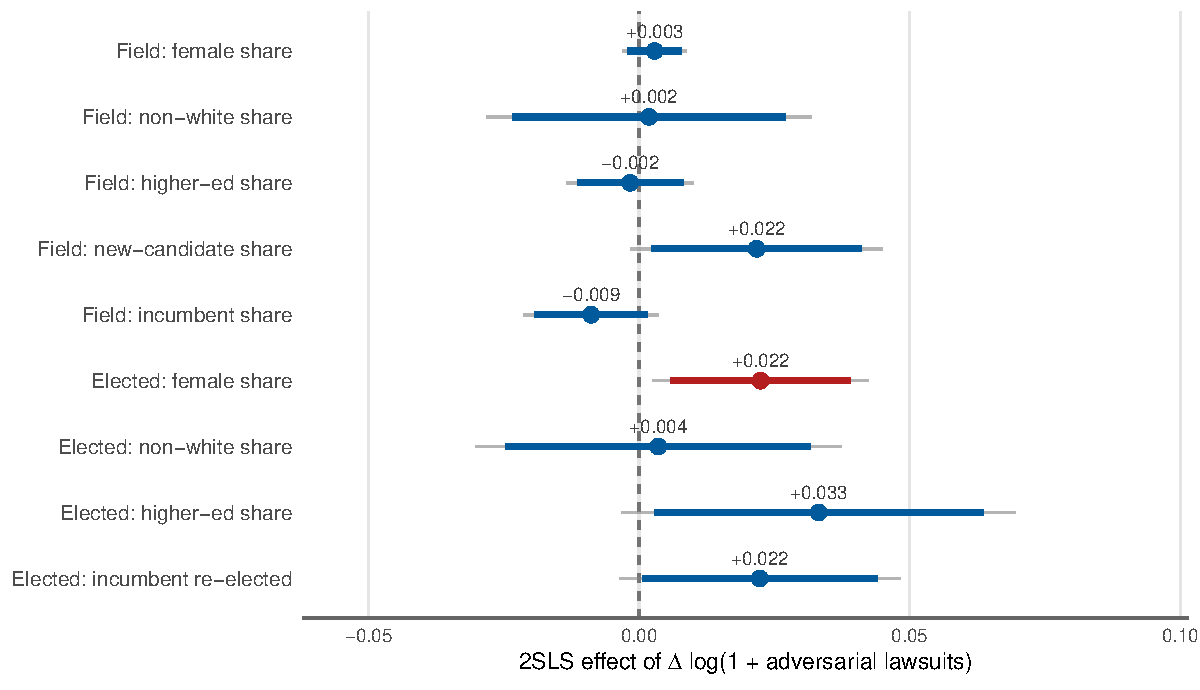
\includegraphics[width=\linewidth,height=0.42\textheight,keepaspectratio]{../figures/legislative_coefplot.pdf}
\end{center}
\smallskip
\takeaway{Of the plotted council outcomes only the elected female share clears 5\% ($\CouncilElFemaleCoef$, $p=\CouncilElFemaleP$); the elected higher-education share ($p=\CouncilElHigherEdP$) and the field's new-candidate share ($p=\CouncilNewCandP$) clear 10\%. Off the plot, the candidate pool is younger (\CouncilAgeYr~yr, $p=\CouncilAgeP$). \CouncilNSig{} of \CouncilNOutcomes{} council outcomes clear 5\%, and no multiplicity correction is computed for the council. Field size ($p=\LegCandP$) and party mix are flat.}\hfill\hyperlink{app:legislative}{\beamergotobutton{Full legislative tables}}\,\hyperlink{app:ballotcouncil}{\beamergotobutton{council ballot}}\,\hyperlink{src:voterballot}{\beamerreturnbutton{Back}}
\end{frame}


\begin{frame}{Appendix --- The Council Ballot Does Not Move}
\hypertarget{app:ballotcouncil}{}
\small
The mayoral ballot result, re-run for the pooled council (vereador) contest. If litigation demobilized voters generally rather than in the single-winner mayoral race specifically, the same blank and null rise and the same valid-vote fall should reappear here. They do not.
\smallskip
\begin{center}
\scriptsize
\resizebox{!}{0.22\textheight}{% Auto-generated by code/03_estimation/02_iv_main.R
% Do not edit manually -- rerun the generating script to update

\begin{tabular}{lccc}
\toprule\toprule
 & \textbf{Blank vote} & \textbf{Null vote} & \textbf{Valid vote} \\
\midrule
\quad \textbf{Judicialization} & $0.000$ & $0.000$ & $-0.003$ \\
 & \textcolor{mygray}{(0.001)} & \textcolor{mygray}{(0.001)} & \textcolor{mygray}{(0.005)} \\
\quad {\footnotesize 2024 Mean} & {\footnotesize 0.013} & {\footnotesize 0.018} & {\footnotesize 0.804} \\
\quad {\footnotesize 2016 Mean} & {\footnotesize 0.015} & {\footnotesize 0.027} & {\footnotesize 0.815} \\[2pt]
\midrule
Municipalities ($N$) & \multicolumn{3}{c}{5,560} \\
\bottomrule\bottomrule
\end{tabular}
}
\end{center}
\smallskip
\footnotesize Every council ballot margin straddles zero: no blank rise, no null rise, no valid-vote erosion. The withdrawal is specific to the mayoral race, where a front-runner is being defended, and is therefore not a board-wide turnout artifact. Outcome is the 2024 rate controlling for the 2016 level; state FE; SEs clustered by state.\hfill\hyperlink{app:councilplacebo}{\beamerreturnbutton{Back}}
\end{frame}


\begin{frame}{Appendix --- The Council Race (full legislative tables)}
\hypertarget{app:legislative}{}
\footnotesize
Full 2SLS estimates behind the council coefficient plot. Two cells are non-null, and neither survives the multiple-testing correction the consolidation clears: the \emph{elected} female share ($+0.022$, $p=.036$) and a marginally \emph{younger} candidate pool (mean age \CouncilAgeYr~yr, $p=\CouncilAgeP$). Field size itself is flat ($\LegCandCoef$, $p=\LegCandP$). Same instrument, built once from the executive design; state FE, clustered by state.
\smallskip

\begin{columns}[T]
\begin{column}{0.5\textwidth}
{\centering\scriptsize\textbf{Candidate pool}\par}
\begin{center}\scriptsize
\resizebox{\linewidth}{!}{% Auto-generated by code/03_estimation/02b_iv_legislative.R
% Do not edit manually -- rerun the generating script to update

\begin{tabular}{lccccccc}
   \tabularnewline \midrule \midrule
   Dependent Variables:                                                     & delta\_log1p\_total\_candidates\_2024\_2020      & delta\_female\_share\_2024\_2020     & delta\_nonwhite\_share\_2024\_2020     & delta\_new\_candidate\_share\_2024\_2020      & delta\_incumbent\_candidate\_share\_2024\_2020      & delta\_effective\_party\_count\_candidates\_2024\_2020       & delta\_candidate\_hhi\_party\_2024\_2020\\       
   Model:                                                                   & (1)                                              & (2)                                  & (3)                                    & (4)                                           & (5)                                                 & (6)                                                          & (7)\\  
   \midrule
   \emph{Variables}\\
   $\Delta$ Log(lawsuits)                                                   & -0.021                                           & 0.005                                & 0.011                                  & -0.002                                        & -0.001                                              & -0.314                                                       & 0.002\\   
                                                                            & (0.043)                                          & (0.005)                              & (0.016)                                & (0.011)                                       & (0.010)                                             & (0.278)                                                      & (0.007)\\   
   \midrule
   \emph{Fixed-effects}\\
   SG\_UF                                                                   & Yes                                              & Yes                                  & Yes                                    & Yes                                           & Yes                                                 & Yes                                                          & Yes\\  
   \midrule
   \emph{Fit statistics}\\
   F-test (1st stage), delta\_log1p\_competition\_lawsuits\_2024\_2020      & 71.4                                             & 71.4                                 & 71.4                                   & 71.4                                          & 71.4                                                & 71.4                                                         & 71.4\\  
   Observations                                                             & 5,560                                            & 5,560                                & 5,560                                  & 5,560                                         & 5,560                                               & 5,560                                                        & 5,560\\  
   \midrule \midrule
   \multicolumn{8}{l}{\emph{Clustered (cluster\_id) standard-errors in parentheses}}\\
   \multicolumn{8}{l}{\emph{Signif. Codes: **: 0.01, *: 0.05, \dagger: 0.1}}\\
\end{tabular}
}
\end{center}
\smallskip

{\centering\scriptsize\textbf{Party composition}\par}
\begin{center}\scriptsize
\resizebox{0.85\linewidth}{!}{% Auto-generated by code/03_estimation/02b_iv_legislative.R
% Do not edit manually -- rerun the generating script to update

\begin{tabular}{l*{2}{c}}
\toprule\toprule
Dep.\ var.: & \textbf{$\Delta$ Party count} & \textbf{$\Delta$ Coalition count} \\
\midrule
\rowcolor{mylight}
\textbf{Judicialization} & -0.212 & -0.070 \\
\rowcolor{mylight}
 & \textcolor{mygray}{(0.299)} & \textcolor{mygray}{(0.056)} \\
\midrule
$N$ & 5,560 & 5,560 \\
Mean of dep.\ var. & 0.275 & 0.767 \\
\bottomrule\bottomrule
\end{tabular}
}
\end{center}
\end{column}
\begin{column}{0.5\textwidth}
{\centering\scriptsize\textbf{Elected composition}\par}
\begin{center}\scriptsize
\resizebox{\linewidth}{!}{% Auto-generated by code/03_estimation/02b_iv_legislative.R
% Do not edit manually -- rerun the generating script to update

\begin{tabular}{lccccc}
   \tabularnewline \midrule \midrule
   Dependent Variables:                                                     & delta\_elected\_female\_share\_2024\_2020      & delta\_elected\_nonwhite\_share\_2024\_2020      & delta\_elected\_higher\_ed\_share\_2024\_2020       & delta\_elected\_mean\_age\_2024\_2020      & delta\_incumbent\_reelected\_share\_2024\_2020\\       
   Model:                                                                   & (1)                                            & (2)                                              & (3)                                                 & (4)                                        & (5)\\  
   \midrule
   \emph{Variables}\\
   $\Delta$ Log(lawsuits)                                                   & 0.013                                          & -0.027                                           & 0.006                                               & 0.039                                      & 0.006\\   
                                                                            & (0.022)                                        & (0.026)                                          & (0.026)                                             & (0.576)                                    & (0.025)\\   
   \midrule
   \emph{Fixed-effects}\\
   SG\_UF                                                                   & Yes                                            & Yes                                              & Yes                                                 & Yes                                        & Yes\\  
   \midrule
   \emph{Fit statistics}\\
   F-test (1st stage), delta\_log1p\_competition\_lawsuits\_2024\_2020      & 235.8                                          & 235.8                                            & 235.8                                               & 235.8                                      & 235.8\\  
   Observations                                                             & 5,560                                          & 5,560                                            & 5,560                                               & 5,560                                      & 5,560\\  
   \midrule \midrule
   \multicolumn{6}{l}{\emph{Clustered (cluster\_id) standard-errors in parentheses}}\\
   \multicolumn{6}{l}{\emph{Signif. Codes: **: 0.01, *: 0.05, \dagger: 0.1}}\\
\end{tabular}
}
\end{center}
\end{column}
\end{columns}
\smallskip
\footnotesize \hfill\hyperlink{app:councilplacebo}{\beamerreturnbutton{Back to figure}}
\end{frame}


\begin{frame}[allowframebreaks]{Appendix --- Summary of All Estimates}
\hypertarget{app:abstract}{}
\footnotesize
Every headline outcome in one table: coefficient, standard error, and the dependent-variable mean, across the consolidation, withdrawal, and null families.
\smallskip
\begin{center}
\scriptsize
% abstract_table.tex — auto-generated by 06_abstract_macros.py
% DO NOT EDIT MANUALLY.

\begin{tabular}{lrrrr}
  \toprule
  Outcome & Coef. & SE & $p$ & Dep.\ mean \\
  \midrule
  \multicolumn{5}{l}{\textit{Panel A: Voter Behavior}} \\
  \quad Turnout (any ballot) & -0.002 & (0.004) & 0.568 & 0.835 \\
  \quad Blank rate (mayoral) & 0.003 & (0.002) & 0.095 & 0.016 \\
  \quad Null rate (mayoral) & 0.003 & (0.002) & 0.120 & 0.027 \\
  \quad Valid rate (mayoral) & -0.007 & (0.006) & 0.277 & 0.792 \\
  \quad Blank rate (council) & 0.000 & (0.001) & 0.455 & 0.013 \\
  \quad Null rate (council) & 0.000 & (0.001) & 0.812 & 0.018 \\
  \quad Valid rate (council) & -0.003 & (0.005) & 0.535 & 0.804 \\
  \midrule
  \multicolumn{5}{l}{\textit{Panel B: Candidate Performance}} \\
  \quad Log candidates (exec.) & -0.007 & (0.016) & 0.677 & -0.112 \\
  \quad $\Delta$ Log candidates (leg.) & 0.021 & (0.032) & 0.515 & -0.108 \\
  \quad Margin (W$-$RU) & 0.062 & (0.023) & 0.013 & 0.270 \\
  \quad Runner-up vote share & -0.032 & (0.012) & 0.016 & 0.337 \\
  \quad Winner majority & 0.057 & (0.036) & 0.124 & 0.832 \\
  \quad $\Delta$ Female candidate share & -0.033 & (0.026) & 0.215 & 0.021 \\
  \quad Female vote share & -0.026 & (0.020) & 0.194 & 0.146 \\
  \quad Winner is female & -0.018 & (0.021) & 0.394 & 0.132 \\
  \midrule
  \multicolumn{5}{l}{\textit{Panel C: Heterogeneity --- Blank Rate (2024)}} \\
  \quad Open seat ($N=2,026$) & 0.001 & (0.002) & 0.571 & 0.014 \\
  \quad Contested ($N=3,534$) & 0.005 & (0.002) & 0.035 & 0.017 \\
  \bottomrule
\end{tabular}
\par\vspace{4pt}
\begin{minipage}{0.97\linewidth}
\footnotesize
\textit{Notes:} Headline estimator: ANCOVA on the 2016 pre-window baseline, $Y_{2024} \sim D + Y_{2016} + X$ (state FE + pre-determined controls), 2SLS with the Bartik instrument. The 2016 level enters as a free lag, so the dependent variable is the 2024 level and ``Dep.\ mean'' is its 2024-level mean. Rows marked $\Delta$ have no clean 2016 analog and are estimated in first differences. First-stage $F=102.3$, $N=5,560$, 26 clusters (states). SE clustered by state (UF). Panel~C open-seat sub-sample first-stage $F=18.6$.
\end{minipage}

\end{center}
\smallskip
\footnotesize \hfill\hyperlink{src:findings}{\beamerreturnbutton{Back}}
\end{frame}

% UNRESOLVED -- these two are src_-prefixed (main-section frames) but sit in
% the appendix run. By the outcome layers they are main-section evidence:
% src_entrant is layer 1 (who runs), src_turnoutprofile is layer 2 (how
% voters respond). Left in place pending the primary-results lock; promoting
% them changes the argument, which is a Results decision, not a spine one.

\begin{frame}{Appendix --- Compositional Neutrality (Mayoral): Renewal and the Entrant Typology}
\hypertarget{src:entrant}{}
\small
\textbf{Mayoral race.} Vote-weighted share going to \textbf{first-time candidates}, \textbf{serial challengers}, and \textbf{cross-cycle returners} --- a finer cut of the renewal-vs-entrenchment question than the binary new/incumbent split. Tests whether judicialization changes the \emph{kind} of entrant the votes flow to. Dots are the 2SLS effect of a one-SD judicialization shock, with 90\% (thick) and weak-IV tF (thin) intervals.
\smallskip
\begin{center}
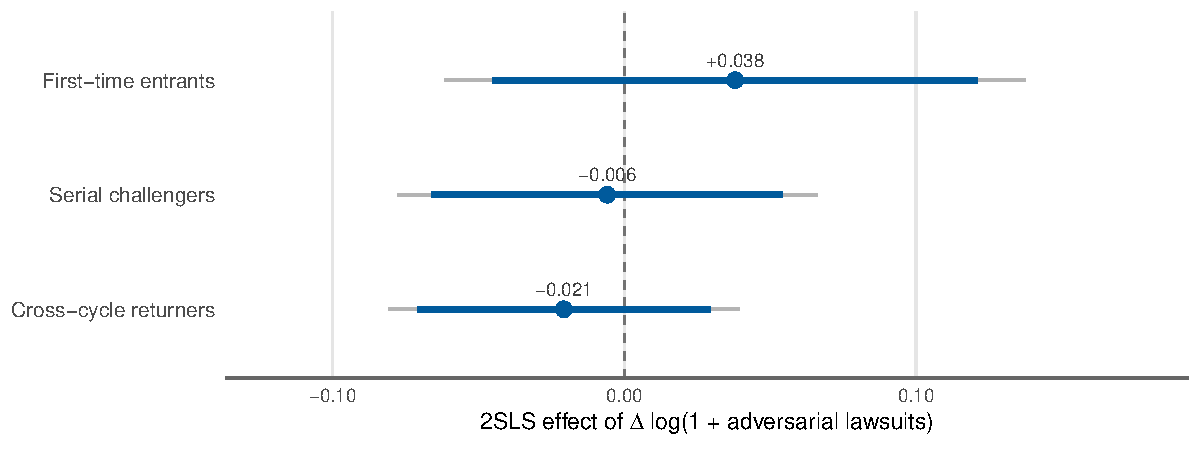
\includegraphics[width=\linewidth,height=0.50\textheight,keepaspectratio]{../figures/entrant_coefplot.pdf}
\end{center}
\smallskip
\footnotesize \textbf{Precise null:} first-timer, serial-challenger, and returner vote shares are all unmoved --- every interval crosses zero. No evidence that litigation shifts the vote toward or away from any class of challenger on net.\hfill\hyperlink{app:entrant}{\beamergotobutton{Full table}}
\end{frame}


\begin{frame}{Appendix --- Entrant Typology (full table)}
\hypertarget{app:entrant}{}
\small
Full 2SLS estimates underlying the coefficient plot: vote-weighted share to first-time entrants, serial challengers, and cross-cycle returners.
\smallskip
\begin{center}
\scriptsize
\resizebox{\linewidth}{!}{% Auto-generated by code/03_estimation/02_iv_main.R
% Do not edit manually -- rerun the generating script to update

\renewcommand{\arraystretch}{1.2}
\begin{tabular}{L{3.8cm}rrr}
  \toprule
  Outcome & Coef. & (SE) & $p$ \\
  \midrule
  $\Delta$ New entrant share & -0.011 & (0.043) & 0.793 \\
  $\Delta$ Serial challenger & 0.007 & (0.026) & 0.802 \\
  $\Delta$ Cross-cycle returner & 0.004 & (0.025) & 0.861 \\
  \midrule
  \multicolumn{4}{l}{\footnotesize N\,=\,5,560, clusters\,=\,2,187, F\,=\,19.6. SE clustered by electoral zone. $^{\dagger}p<0.10$, $^{*}p<0.05$, $^{**}p<0.01$.} \\
  \bottomrule
\end{tabular}
}
\end{center}
\smallskip
\footnotesize \hfill\hyperlink{src:entrant}{\beamerreturnbutton{Back to figure}}
\end{frame}


\begin{frame}{Appendix --- Heterogeneity by Seat Type (full mayoral table)}
\hypertarget{app:seathet}{}
\small
The full mayoral split behind the two-channel figure: each consolidation and withdrawal outcome estimated separately on open seats (incumbent term-limited, $N=\OpenN$) and contested seats (incumbent eligible, $N=\ContN$). Shaded row = headline top-two margin; State (UF) FE; SEs clustered by state.
\vspace{-2pt}
\begin{center}
\scriptsize
\resizebox{!}{0.29\textheight}{% Auto-generated by code/03_estimation/02_iv_main.R
% Do not edit manually -- rerun the generating script to update

\begin{tabular}{lccc}
\toprule\toprule
 & \textbf{Open seat} & \textbf{Contested} & 2024 Mean \\
 & {\footnotesize (term-limited)} & {\footnotesize (incumbent)} & \\
\midrule
\multicolumn{4}{l}{\emph{Consolidation}}\\[1pt]
\rowcolor{mylight}
\quad \textbf{Winner's top-two margin} & $0.076$$^{**}$ & $0.068$$^{**}$ & 0.270 \\
\rowcolor{mylight}
 & \textcolor{mygray}{(0.037)} & \textcolor{mygray}{(0.024)} & \\
\quad Winner vote share & $0.039$$^{*}$ & $0.033$$^{**}$ & 0.607 \\
 & \textcolor{mygray}{(0.020)} & \textcolor{mygray}{(0.013)} & \\
\quad Winner majority ($>$50\%) & $0.160$$^{*}$ & $0.011$ & 0.832 \\
 & \textcolor{mygray}{(0.081)} & \textcolor{mygray}{(0.033)} & \\
\addlinespace[2pt]
\multicolumn{4}{l}{\emph{Voter disengagement}}\\[1pt]
\quad Blank-vote rate & $0.001$ & $0.005$$^{**}$ & 0.016 \\
 & \textcolor{mygray}{(0.002)} & \textcolor{mygray}{(0.002)} & \\
\quad Null-vote rate & $0.004$ & $0.003$ & 0.027 \\
 & \textcolor{mygray}{(0.003)} & \textcolor{mygray}{(0.002)} & \\
\quad Valid-vote rate & $0.004$ & $-0.013$$^{*}$ & 0.792 \\
 & \textcolor{mygray}{(0.009)} & \textcolor{mygray}{(0.007)} & \\
\midrule
$N$ & 2,026 & 3,534 & \\
\bottomrule\bottomrule
\end{tabular}
}
\end{center}
\vspace{-2pt}
\footnotesize The top-two margin widens in both columns. The winner-majority indicator moves only for open seats, while the blank rise ($p=\ContBlankP$) and the valid-vote fall ($p=\ContValidP$) appear only in contested seats, so the two channels sort by whether an incumbent is defending. The open-seat margin already widened before 2020 (pre-trend $p=\OpenPtMarginP$).\hfill\hyperlink{app:seatdisengage}{\beamergotobutton{by office}}\,\hyperlink{src:seathet}{\beamerreturnbutton{Back}}
\end{frame}


\begin{frame}{Appendix --- Voter Withdrawal by Seat Type and Office}
\hypertarget{app:seatdisengage}{}
\small
The mayoral seat split places the withdrawal in contested races. The table below asks whether it also separates the two offices: if litigation demobilizes the high-stakes mayoral contest, the low-salience council ballot should not move in step (open $N=\OpenN$, contested $N=\ContN$).
\vspace{-2pt}
\begin{center}
\scriptsize
\resizebox{!}{0.32\textheight}{% Auto-generated by code/03_estimation/02_iv_main.R
% Do not edit manually -- rerun the generating script to update

\begin{tabular}{lcccc}
\toprule\toprule
 & \textbf{Blank vote} & \textbf{Null vote} & \textbf{Valid vote} & $N$ \\
\midrule
\multicolumn{5}{l}{\emph{Mayoral (prefeito)}}\\[1pt]
\quad Open seat & $0.003$ & $0.004$ & $0.006$ & 1,994 \\
 & \textcolor{mygray}{(0.002)} & \textcolor{mygray}{(0.004)} & \textcolor{mygray}{(0.010)} & \\
\rowcolor{mylight}
\quad \textbf{Contested} & $0.007$$^{***}$ & $0.006$$^{**}$ & $-0.023$$^{***}$ & 3,566 \\
\rowcolor{mylight}
 & \textcolor{mygray}{(0.002)} & \textcolor{mygray}{(0.003)} & \textcolor{mygray}{(0.007)} & \\
\addlinespace[2pt]
\multicolumn{5}{l}{\emph{Council (vereador)}}\\[1pt]
\quad Open seat & $0.000$ & $-0.001$ & $0.012$ & 1,994 \\
 & \textcolor{mygray}{(0.001)} & \textcolor{mygray}{(0.001)} & \textcolor{mygray}{(0.008)} & \\
\quad Contested & $0.001$ & $0.000$ & $-0.015$$^{***}$ & 3,566 \\
 & \textcolor{mygray}{(0.001)} & \textcolor{mygray}{(0.001)} & \textcolor{mygray}{(0.005)} & \\
\midrule
\emph{2024 mean (mayoral)} & 0.016 & 0.027 & 0.792 & \\
\emph{2024 mean (council)} & 0.013 & 0.018 & 0.804 & \\
\bottomrule\bottomrule
\end{tabular}
}
\end{center}
\vspace{-2pt}
\footnotesize The shaded contested-mayoral row carries the effect: blanks rise ($p=\ContBlankP$) and valid votes fall ($p=\ContValidP$), while the null rate does not move significantly. The council shows at most a faint valid-vote dip without that accompanying rise, which is the opposite of what a low-stakes, open-seat account would predict. Campaign spending is examined next as an alternative channel.\hfill\hyperlink{app:spending}{\beamergotobutton{spending}}\,\hyperlink{app:seathet}{\beamerreturnbutton{Back}}
\end{frame}


\begin{frame}{Appendix --- Turnout Placebo (compulsory vote)}
\hypertarget{app:turnoutplacebo}{}
\small
Turnout is one act per voter, so it is office-invariant and reported here on its own. Because voting is compulsory in Brazil, overall turnout is institutionally floored and should not respond to litigation, which makes it a placebo. A near-zero, insignificant coefficient is what a valid design should deliver, since it shows the instrument is not picking up an omitted municipal shock that moves all electoral behavior at once. The elastic facultative turnout margins that can move are tested separately \hyperlink{src:turnoutprofile}{\beamergotobutton{by voter profile}}.
\smallskip
\begin{center}
\scriptsize
\resizebox{0.6\linewidth}{!}{% Auto-generated by code/03_estimation/02_iv_main.R
% Do not edit manually -- rerun the generating script to update

\begin{tabular}{lc}
   \tabularnewline \midrule \midrule
   Dependent Variable: & Turnout (any ballot)\\  
   Model:              & (1)\\  
   Judicialization     & -0.006\\   
                       & (0.004)\\   
   2024 Mean           & 0.835\\  
   2016 Mean           & 0.856\\  
   \midrule \midrule
   \multicolumn{2}{l}{\emph{Clustered (state) standard-errors in parentheses}}\\
   \multicolumn{2}{l}{\emph{Signif. Codes: ***: 0.01, **: 0.05, *: 0.1}}\\
\end{tabular}
}
\end{center}
\smallskip
\footnotesize The coefficient is indistinguishable from zero ($\TurnoutCoef$, $p=\TurnoutP$). Two caveats: turnout fails the pre-trend placebo ($p=\PtRFTurnoutP$), and compulsory turnout, measured separately, rises ($\CompulsoryCoef$, $p=\CompulsoryP$, tF interval excludes zero). Outcome is the 2024 turnout rate controlling for the 2016 level; state (UF) FE; SEs clustered by state.\hfill\hyperlink{src:voterballot}{\beamerreturnbutton{Back}}
\end{frame}


\begin{frame}{Appendix --- Voter Behavior: Turnout by Voter Profile}
\hypertarget{src:turnoutprofile}{}
\small
Compulsory turnout is mechanically frozen, but turnout among the \textbf{facultative} electorate (ages 16--17 and 70$+$) is free to move (it rose from \TurnoutRateTwenty\% to \TurnoutRateFortyFour\% overall, with far larger municipal swings), and turnout has a strong \textbf{education gradient}. If litigation demobilizes, these elastic margins are where it should show. Each dot is the 2SLS effect of a one-SD shock; bars are 90\% (thick) and weak-IV (tF, thin) intervals. From the TSE \emph{perfil do eleitorado}; state FE, clustered by state.
\smallskip
\begin{center}
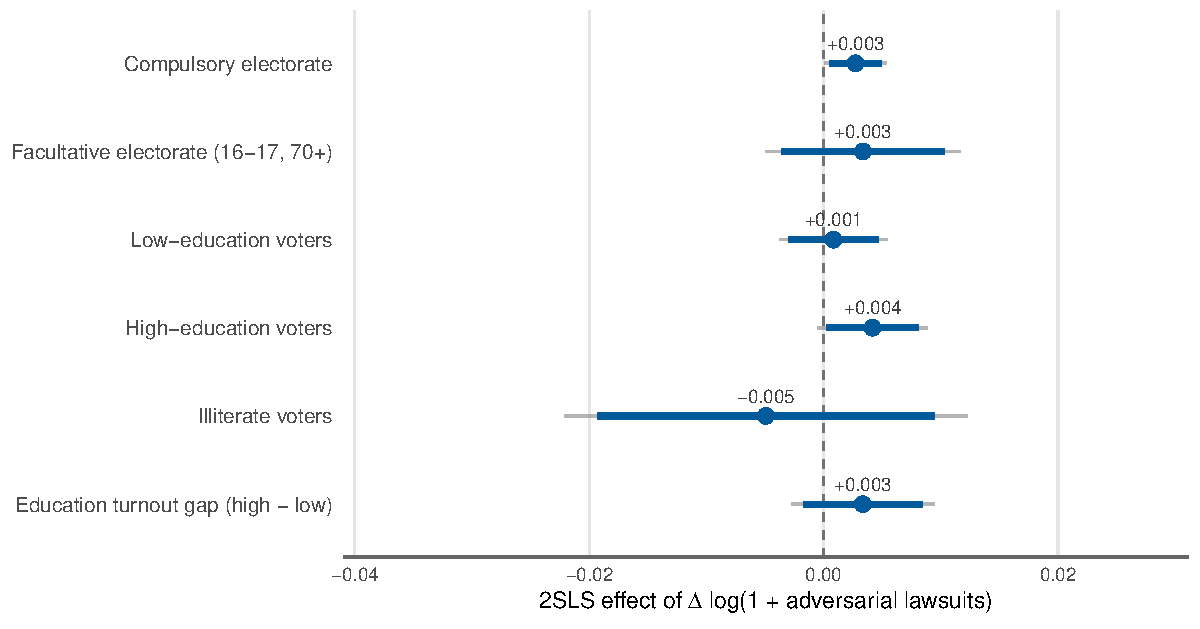
\includegraphics[width=\linewidth,height=0.48\textheight,keepaspectratio]{../figures/turnout_coefplot.pdf}
\end{center}
\smallskip
\footnotesize \textbf{Null on every margin.} Every interval crosses zero and the magnitudes are negligible: a one-SD rise in judicialization ($\approx\TreatSDMult\times$ more litigation) moves facultative turnout by only $\FacultativePerSDSigned$~pp and the education gap by $\EduGapPerSDSigned$~pp, both indistinguishable from zero. The high-education margin is closest to a signal ($p=\HighEdP$) but does not clear conventional significance.\hfill\hyperlink{app:turnoutprofile}{\beamergotobutton{Full table}}
\end{frame}


\begin{frame}{Appendix --- Turnout by Voter Profile (full table)}
\hypertarget{app:turnoutprofile}{}
\small
Full 2SLS estimates underlying the coefficient plot: turnout response by electorate type and education stratum. Disaggregated from the TSE \emph{perfil do eleitorado}; state FE; clustered by state.
\smallskip
\begin{center}
\scriptsize
\renewcommand{\arraystretch}{1.25}
\begin{tabular}{lccc}
  \toprule
  $\Delta$ Turnout outcome & Coef. & SE & $p$ \\
  \midrule
  Compulsory electorate          & \CompulsoryCoef  & \CompulsorySE  & \CompulsoryP \\
  Facultative electorate         & \FacultativeCoef & \FacultativeSE & \FacultativeP \\
  Low-education voters           & \LowEdCoef       & \LowEdSE       & \LowEdP \\
  High-education voters          & \HighEdCoef      & \HighEdSE      & \HighEdP \\
  Illiterate (\emph{analfabeto}) & \AnalfabetoCoef  & \AnalfabetoSE  & \AnalfabetoP \\
  \midrule
  Education turnout gap (high $-$ low) & \EduGapCoef & \EduGapSE & \EduGapP \\
  \bottomrule
\end{tabular}
\end{center}
\smallskip
\footnotesize\hfill\hyperlink{src:turnoutprofile}{\beamerreturnbutton{Back to figure}}
\end{frame}



% ============================================================
\section{References}
\begin{frame}[allowframebreaks]{References}
\hypertarget{src:references}{}
\footnotesize
\bibliographystyle{plainnat}
\bibliography{biblio}
\end{frame}


\end{document}
